\begin{frame}{Simulation}
    \begin{figure}
        \centering
        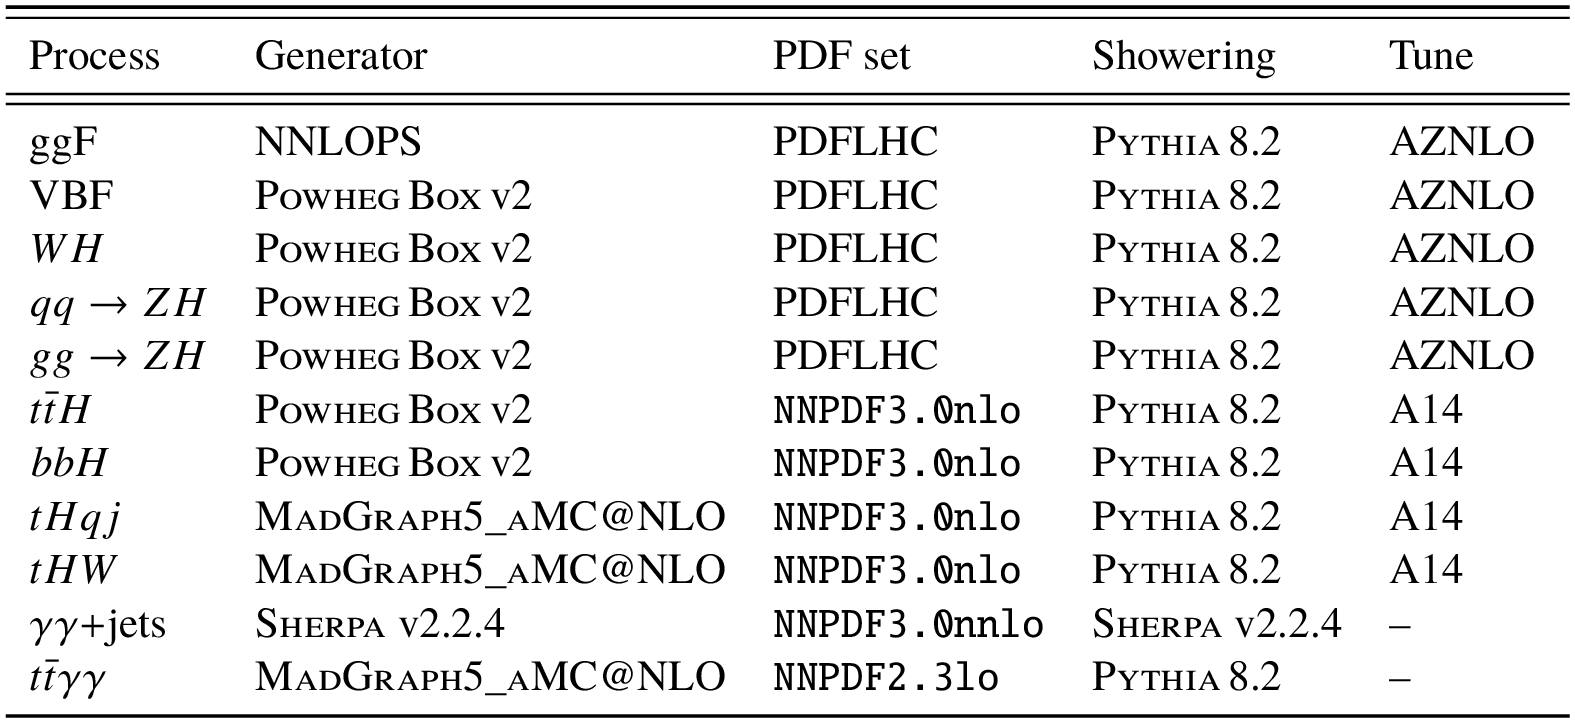
\includegraphics[width=0.8\textwidth]{BackUp/Part3/Img/Single_Higgs_samples.png}
    \end{figure}
\end{frame}
\begin{frame}{Di-photon trigger efficiency}
\begin{figure}
    \centering
    \subfloat{ 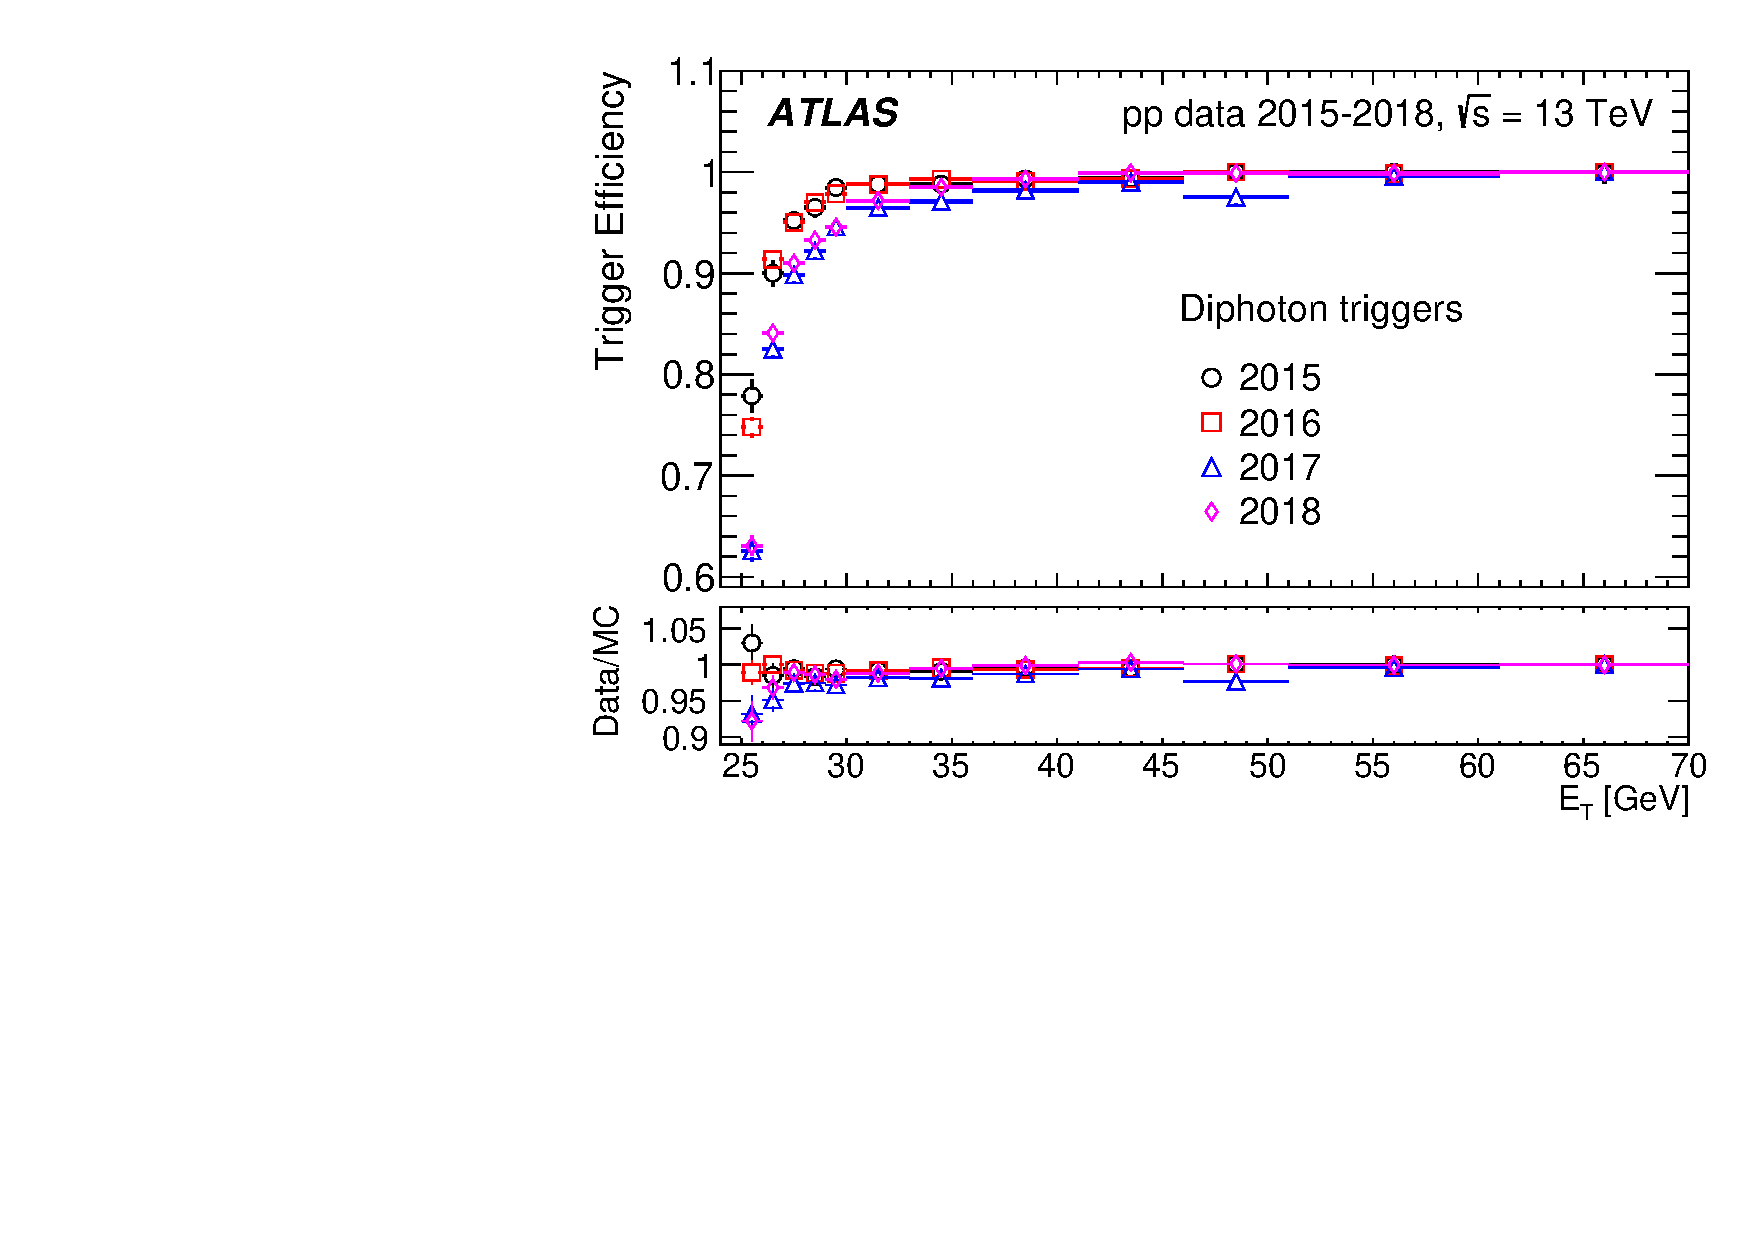
\includegraphics[width=0.5\textwidth]{BackUp/Part3/Img/Trigger_Et.pdf}}
    \subfloat{ 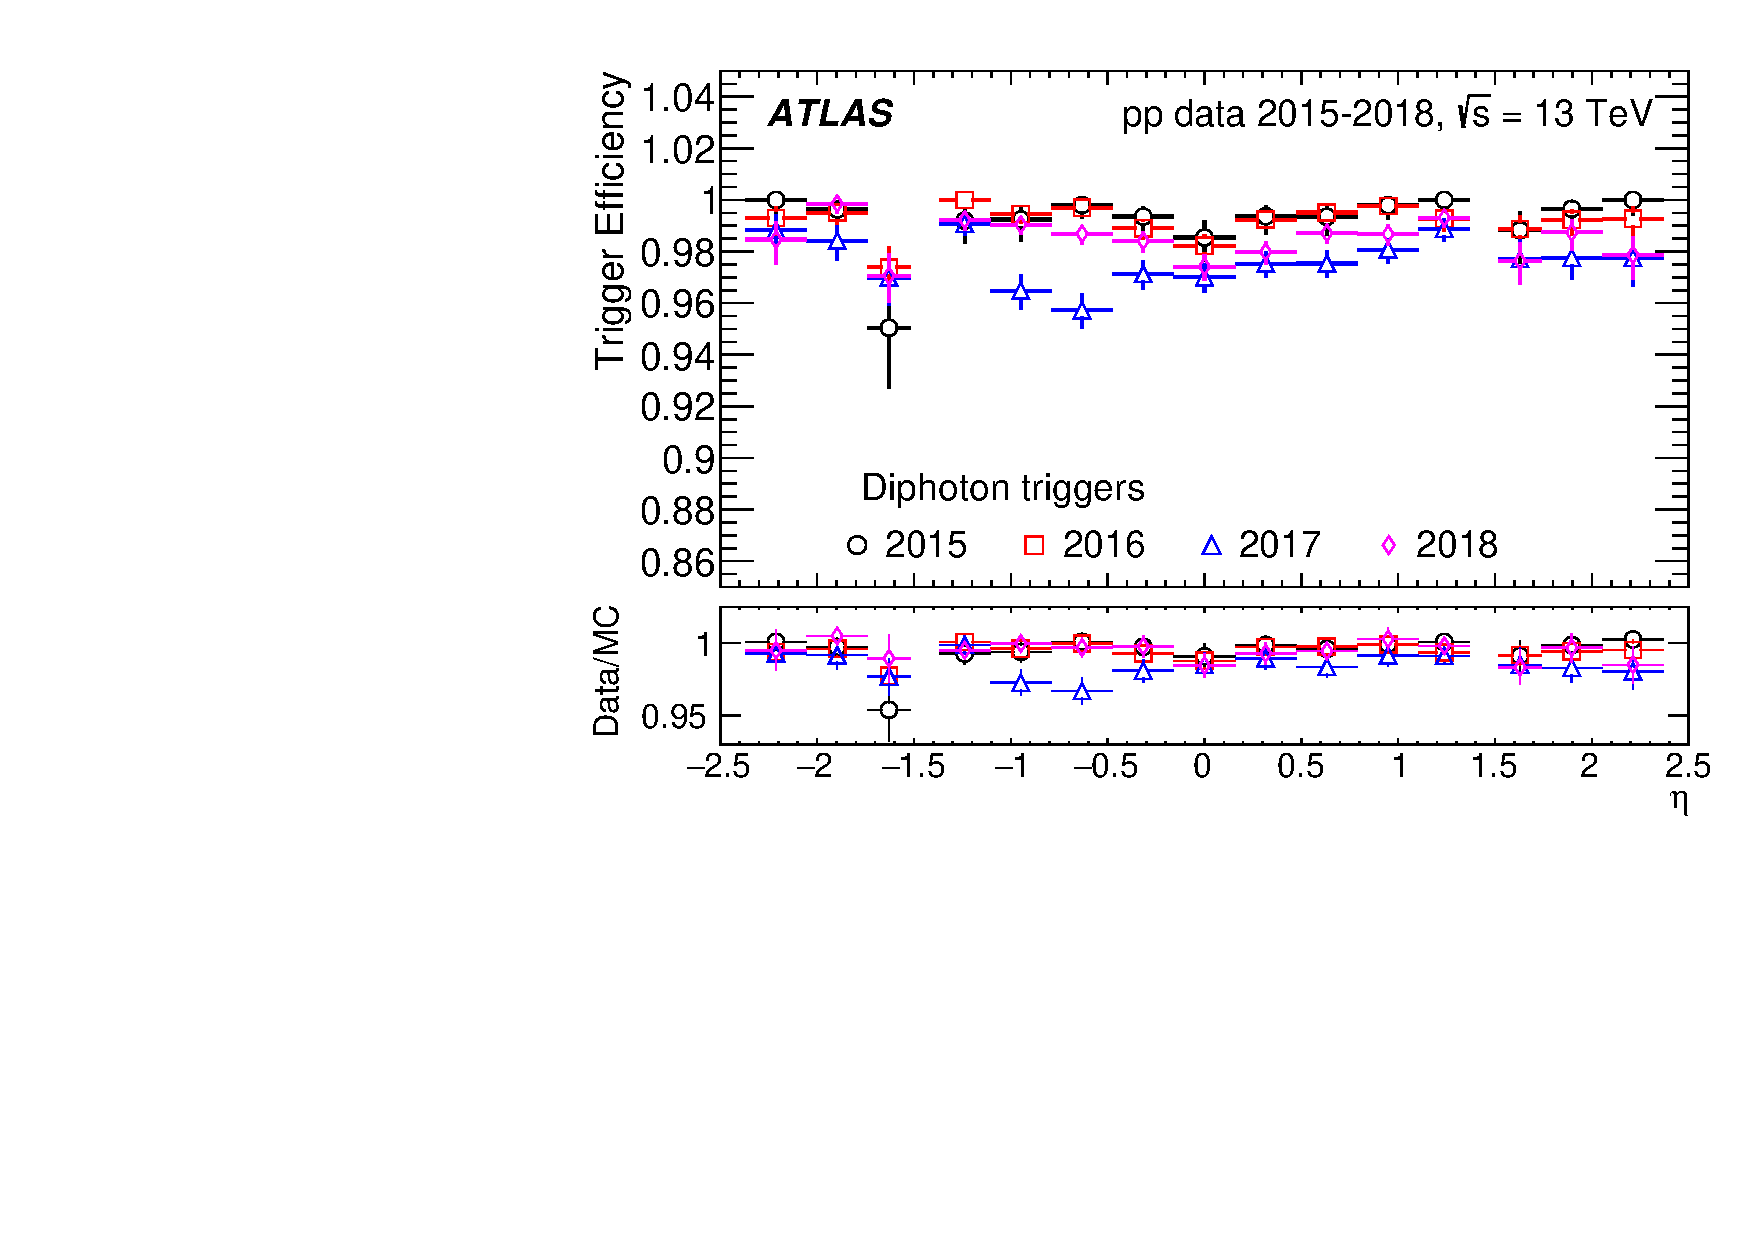
\includegraphics[width=0.5\textwidth]{BackUp/Part3/Img/Trigger_Eta.pdf}}
\end{figure}
\end{frame}

\begin{frame}{$b$-jet calibration chain}
    \begin{figure}
        \centering
        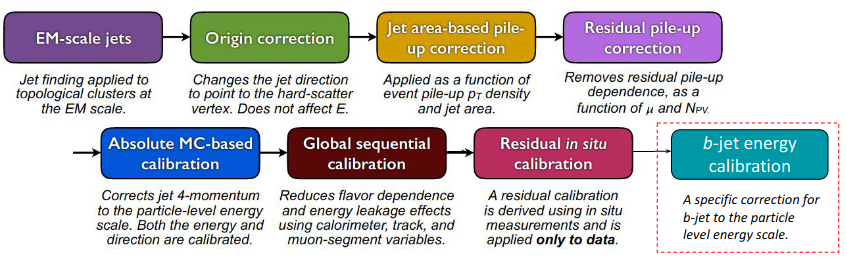
\includegraphics[width=0.8\textwidth]{BackUp/Part3/Img/b_jet_chain.png}
    \end{figure}
\end{frame}

\begin{frame}{$\mu$-in-jet correction selection}

\begin{columns}
\column{0.5\textwidth}
\begin{table}[h]
    \centering
    \begin{tabular}{ll}
    \hline\hline
        Criteria & Selection \\
    \hline    
        $p_T$ & $>$ 4 GeV \\
        ID & Medium \\
        $\Delta R$ & $< \min(0.4, 0.004 + 10/p_T)$ \\
        \hline\hline
    \end{tabular}
\end{table}
\column{0.5\textwidth}

\begin{figure}
    \centering
    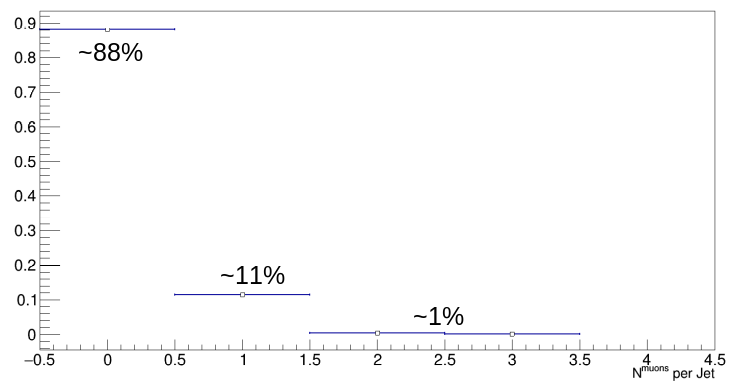
\includegraphics[width=1.\textwidth]{BackUp/Part3/Img/Number_of_muon.png}
\end{figure}
\end{columns}
\end{frame}

\begin{frame}{$p_T$Reco correction}
\begin{columns}
\column{0.5\textwidth}
\begin{itemize}
    \item Target $\to$ \textit{TruthWZ} jets, contains reconstructed jets with all stable hadrons and non-isolated muons and neutrinos. $\Delta R(jet^{truth}, jet^{reco})$
    \item Correction = mean of the $\frac{p_T^{truth}}{p_T^{reco}}$ distribution
\end{itemize}

\column{0.5\textwidth}
\begin{figure}
    \centering
    \subfloat{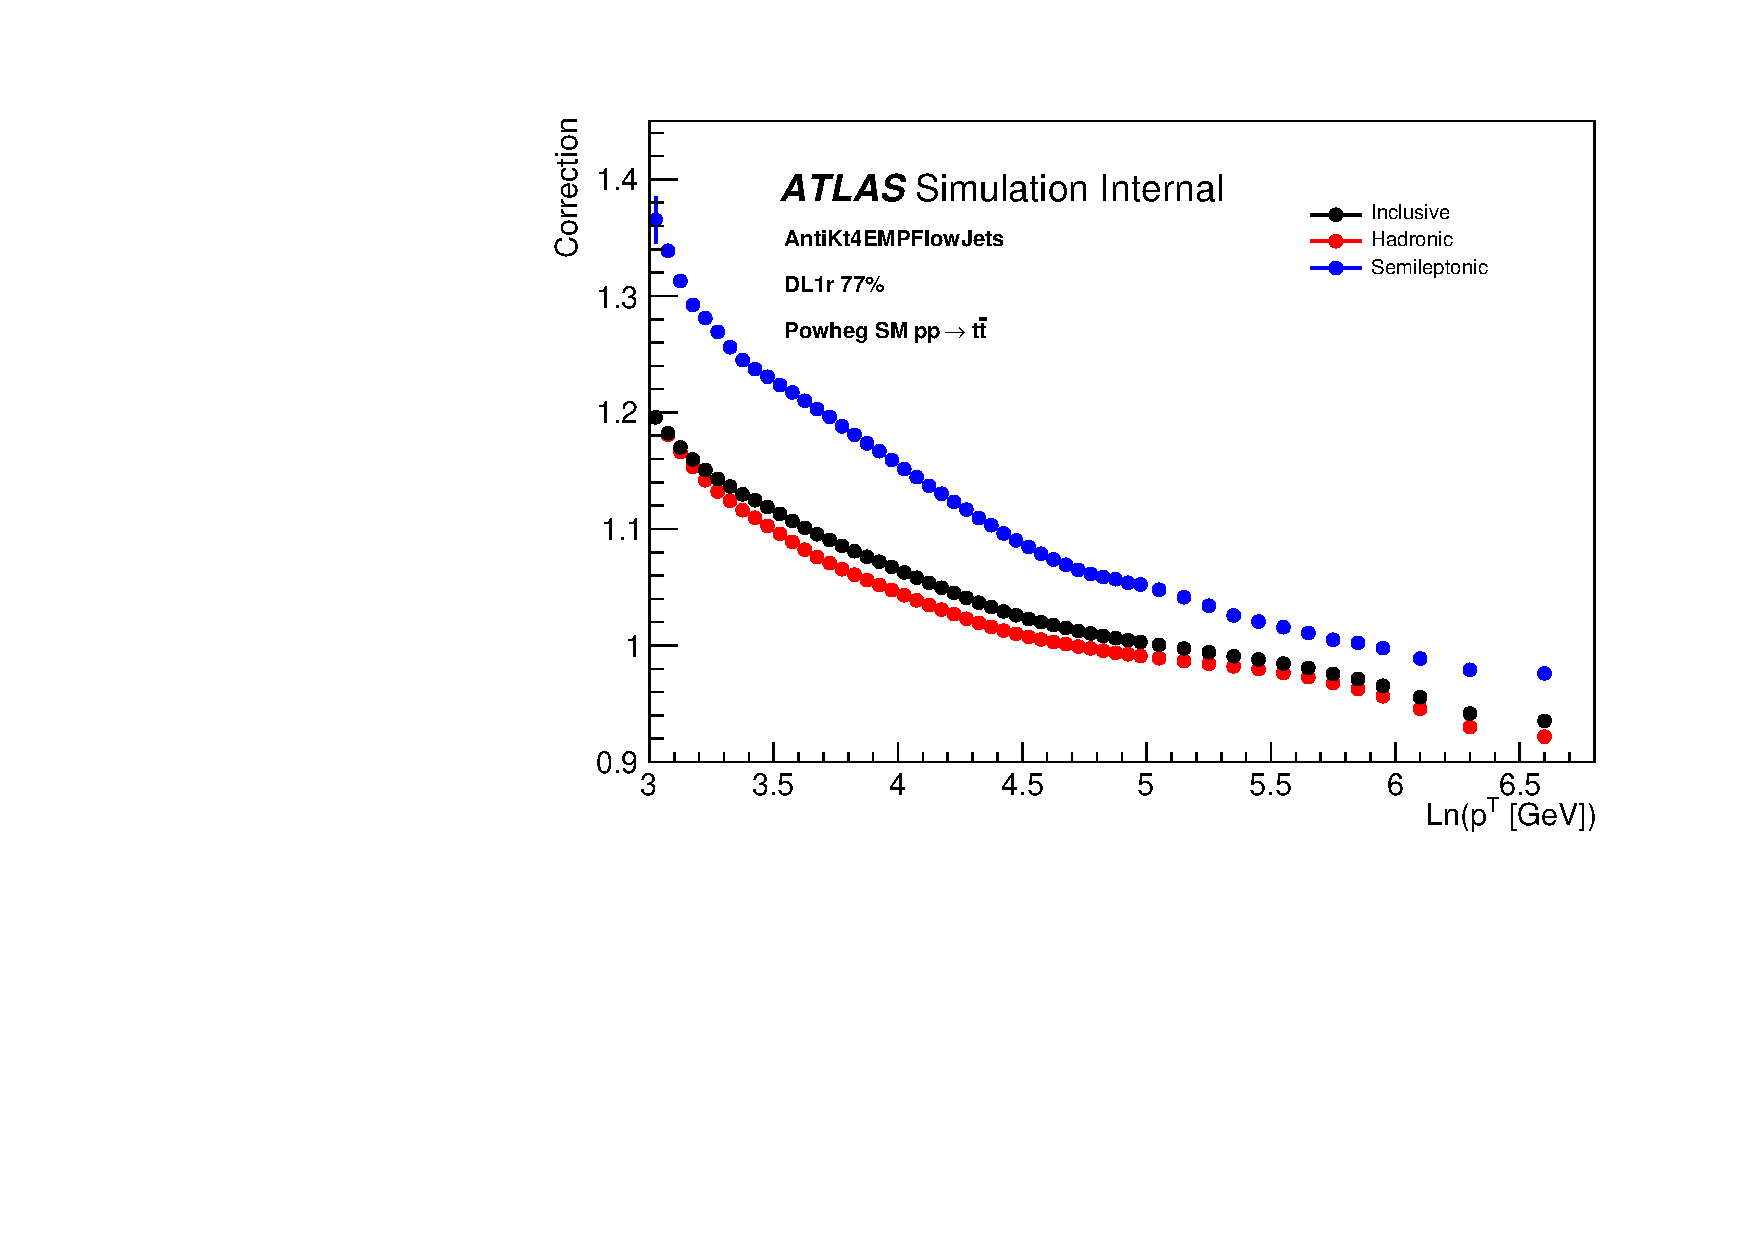
\includegraphics[width=0.75\textwidth]{BackUp/Part3/Img/PtRec_AntiKt4EMPFlowJets.pdf}}\\
    \subfloat{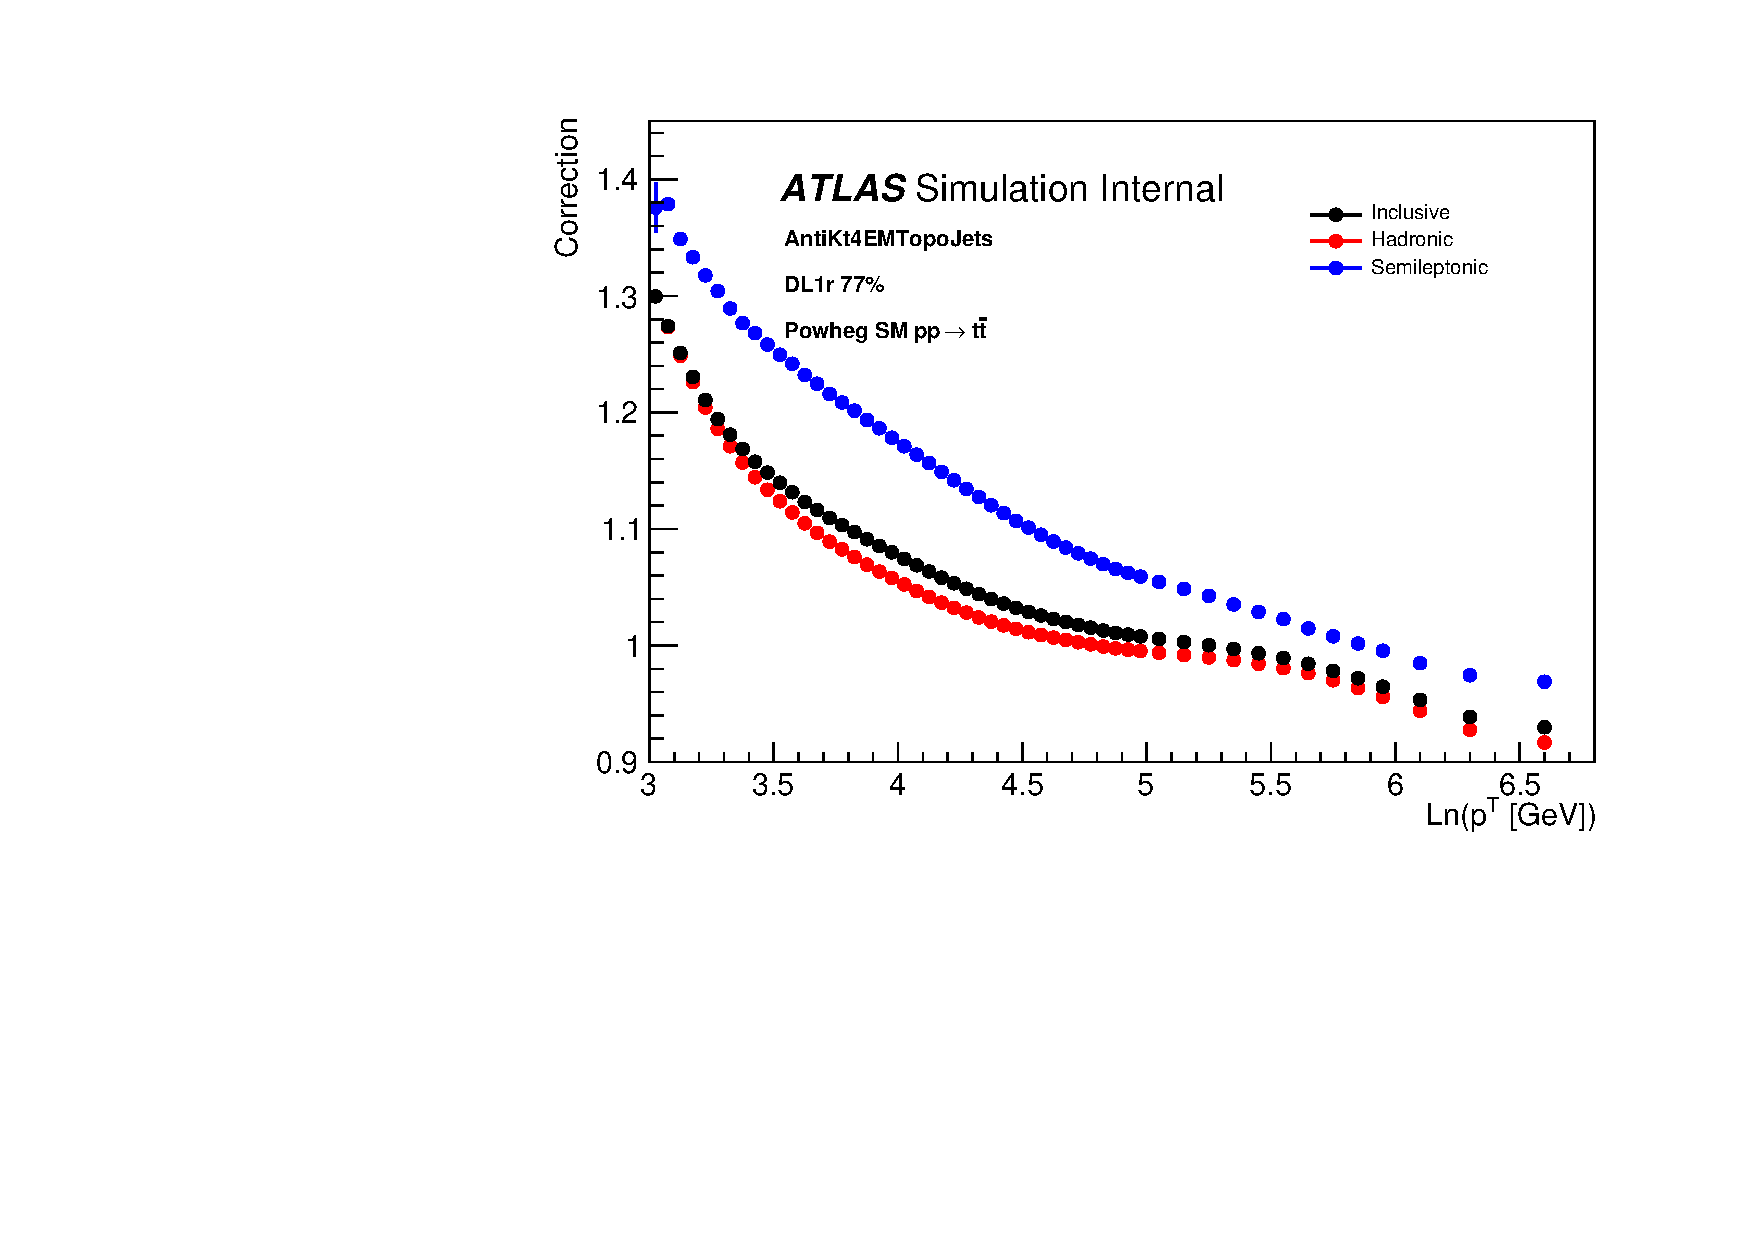
\includegraphics[width=0.75\textwidth]{BackUp/Part3/Img/PtRec_AntiKt4EMTopoJets.pdf}}
\end{figure}
\end{columns}
\end{frame}

\begin{frame}{$p_T$Reco gain}
\begin{figure}
    \centering
    \subfloat{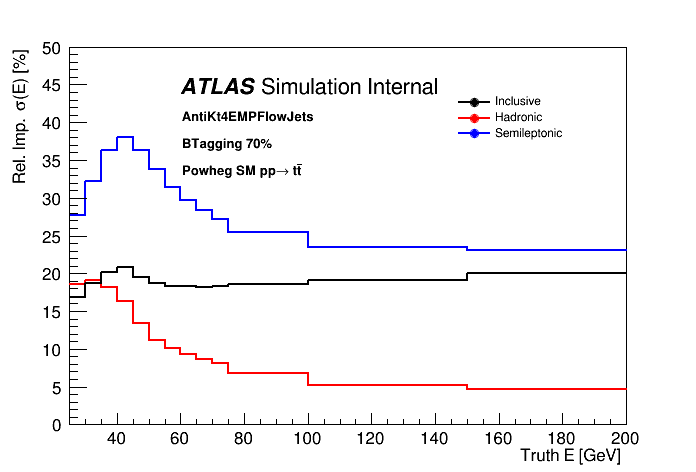
\includegraphics[width=0.5\textwidth]{BackUp/Part3/Img/E_AntiKt4EMPFlowJets.png}}
    \subfloat{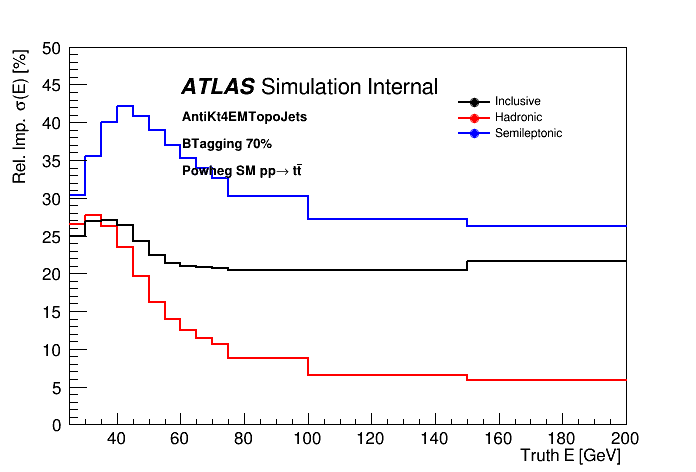
\includegraphics[width=0.5\textwidth]{BackUp/Part3/Img/E_AntiKt4EMTopoJets.png}}
\end{figure}
\end{frame}

\begin{frame}{$m_{bb}$ correction in each step}
\begin{figure}
    \centering
    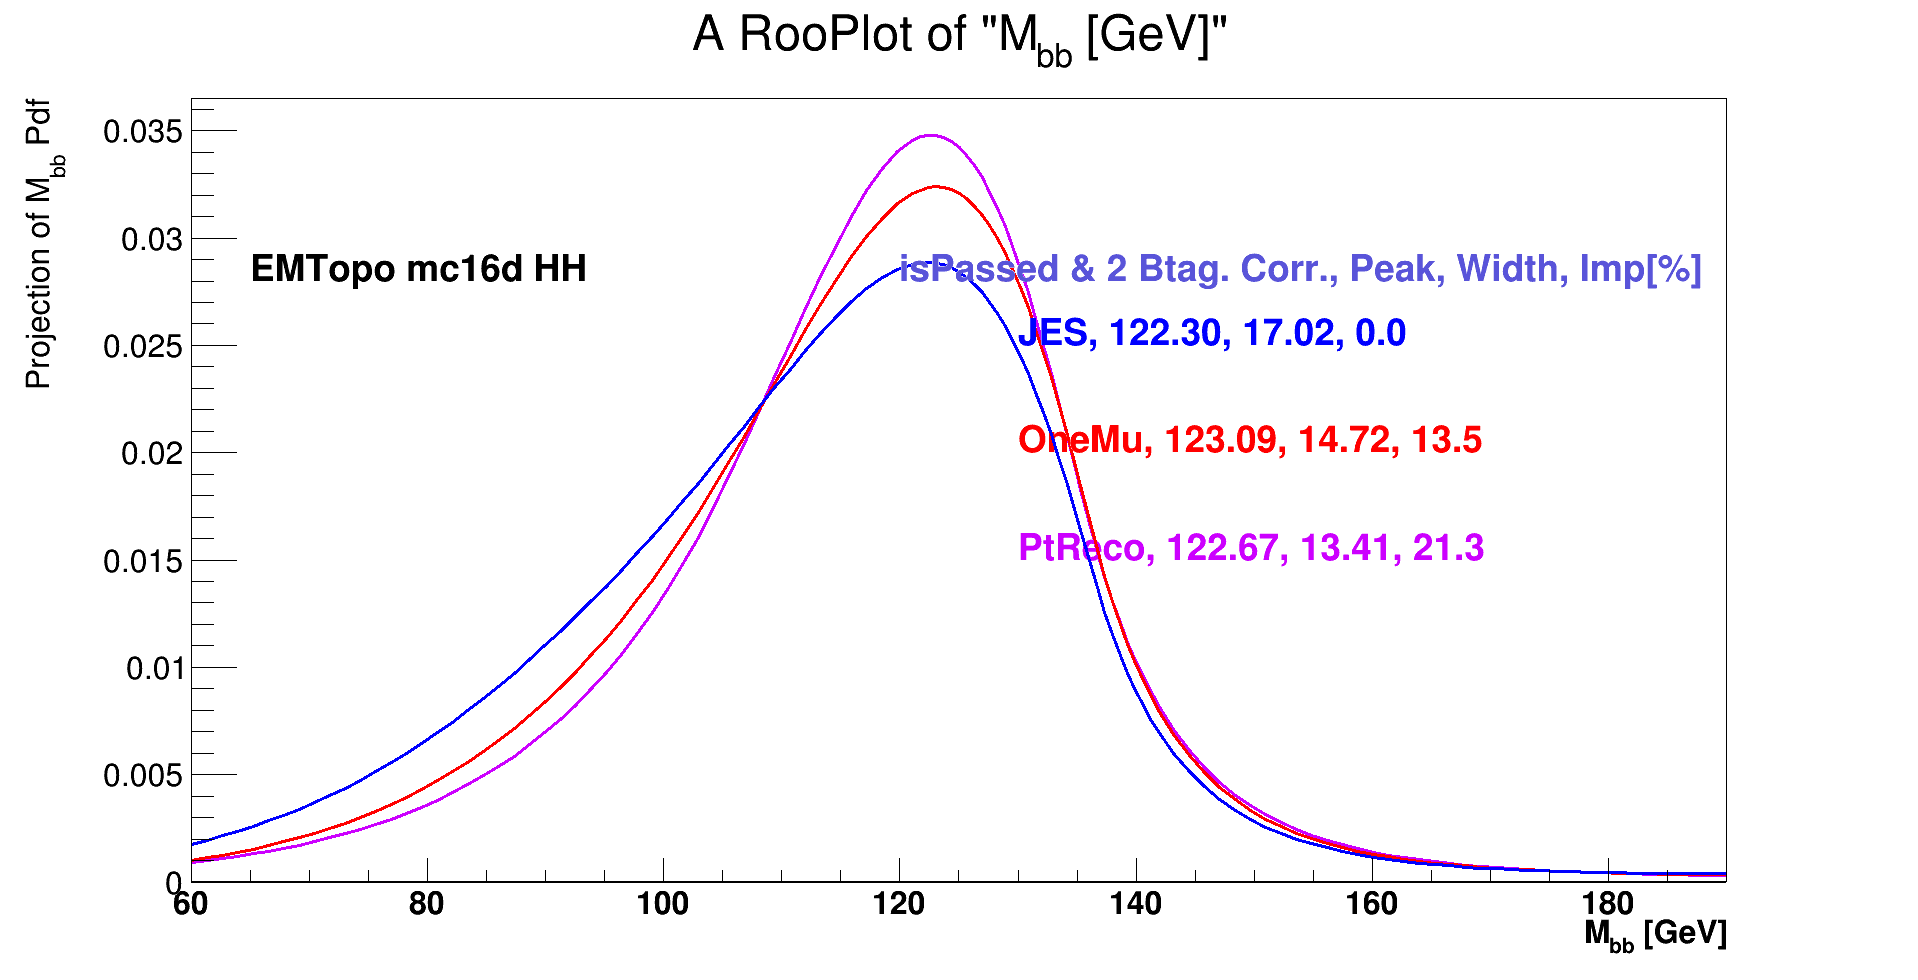
\includegraphics[width=0.8\textwidth]{BackUp/Part3/Img/mbb_PtReco_HH.png}
\end{figure}    
\end{frame}

\begin{frame}{topological vs particle flow $m_{bb}$}
\begin{figure}
    \centering
    \subfloat{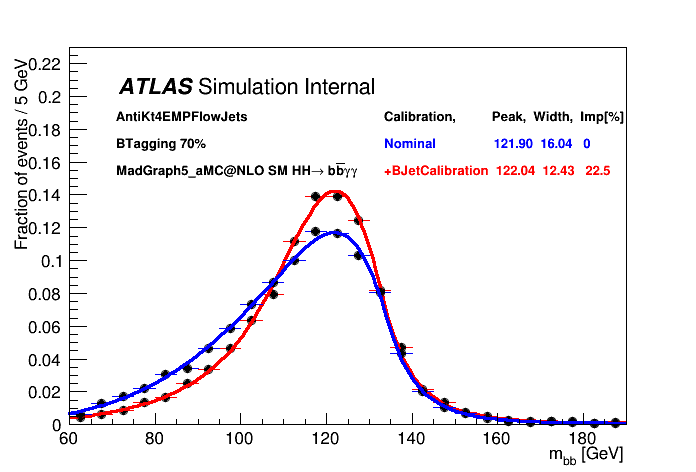
\includegraphics[width=0.5\textwidth]{BackUp/Part3/Img/mbb_AntiKt4EMPFlowJets.png}}
    \subfloat{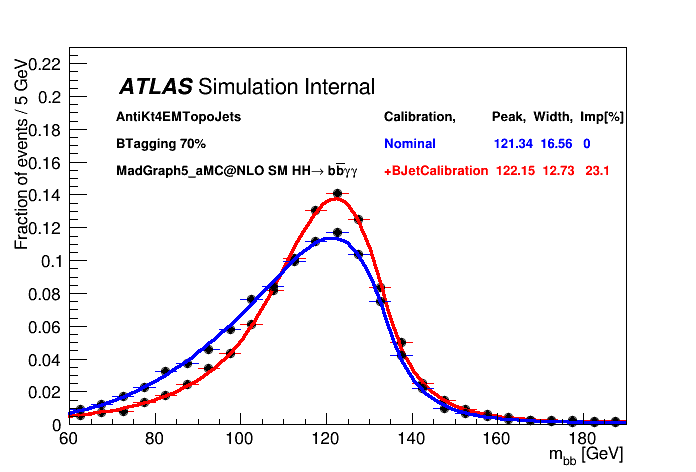
\includegraphics[width=0.5\textwidth]{BackUp/Part3/Img/mbb_AntiKt4EMTopoJets.png}}
\end{figure}
\end{frame}

\begin{frame}{Impact on ZH background}
    \begin{figure}
        \centering
        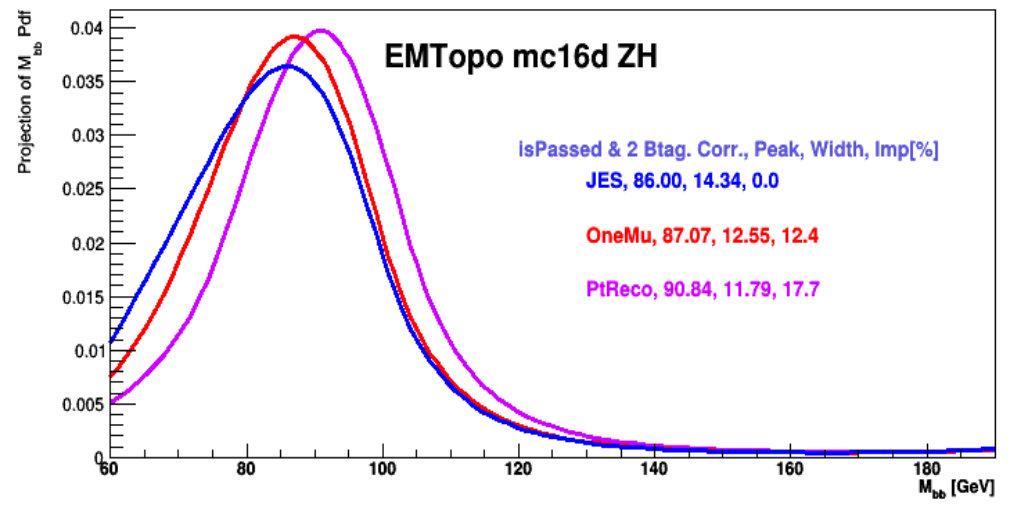
\includegraphics[width=0.6\textwidth]{BackUp/Part3/Img/ZH_b_jets_cal.png}
    \end{figure}
\end{frame}

\begin{frame}{Impact on $t\bar{t}$H background}
    \begin{figure}
        \centering
        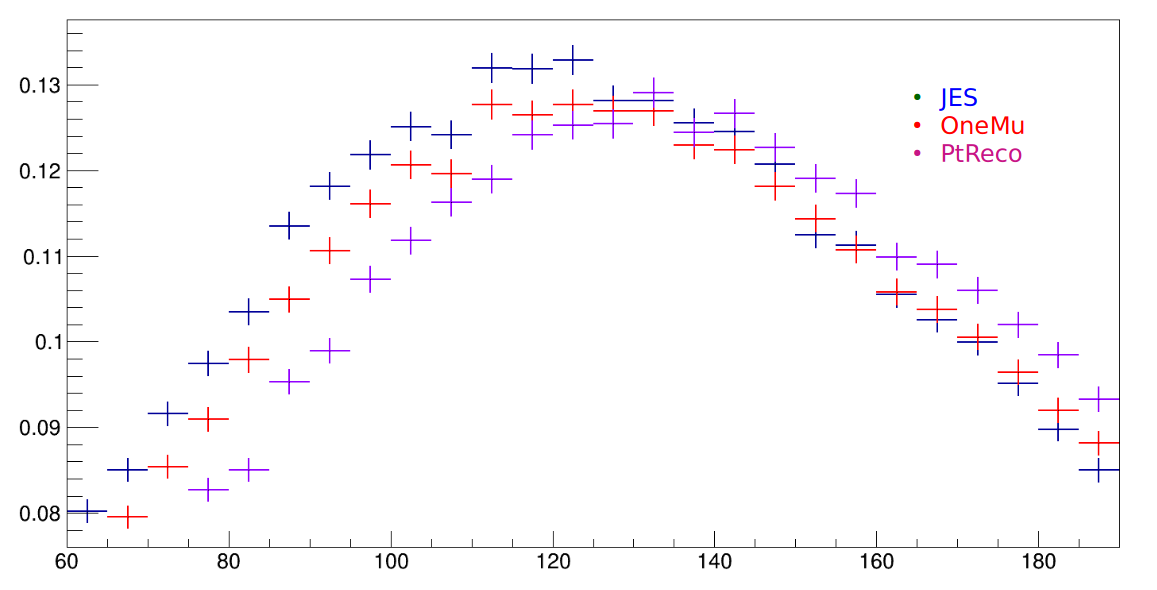
\includegraphics[width=0.6\textwidth]{BackUp/Part3/Img/ttH_b_jets_cal.png}
    \end{figure}
\end{frame}

%\begin{frame}{Impact on continuum $\gamma\gamma$+jets background}
    
%\end{frame}

\begin{frame}{Neural Network vs $\mu$-in-jet+$p_T$Reco}

\begin{itemize}
    \item $\mu$-in-jet+$p_T$Reco compared to simple NN version. 
    \item NN trained on $t\bar{t}$ sample
    \item Comparison performed on HH$\to b\bar{b} b\bar{b}$
\end{itemize}
\begin{figure}
    \centering
    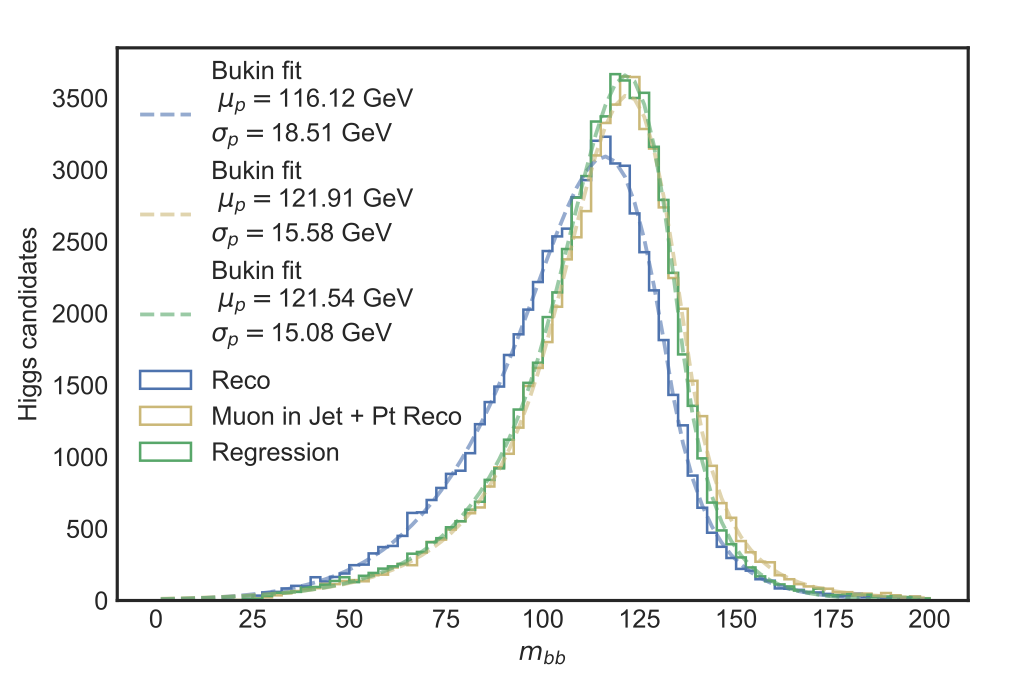
\includegraphics[width=0.6\textwidth]{BackUp/Part3/Img/4b_NN_vs_PtReco.png}
\end{figure}
\end{frame}

\begin{frame}{Motivation for $m_{b\bar{b}\gamma\gamma}^*$}
\begin{itemize}
    \item Improve resolution mainly for resonance analysis
\end{itemize}
\begin{figure}
        \centering
        \subfloat{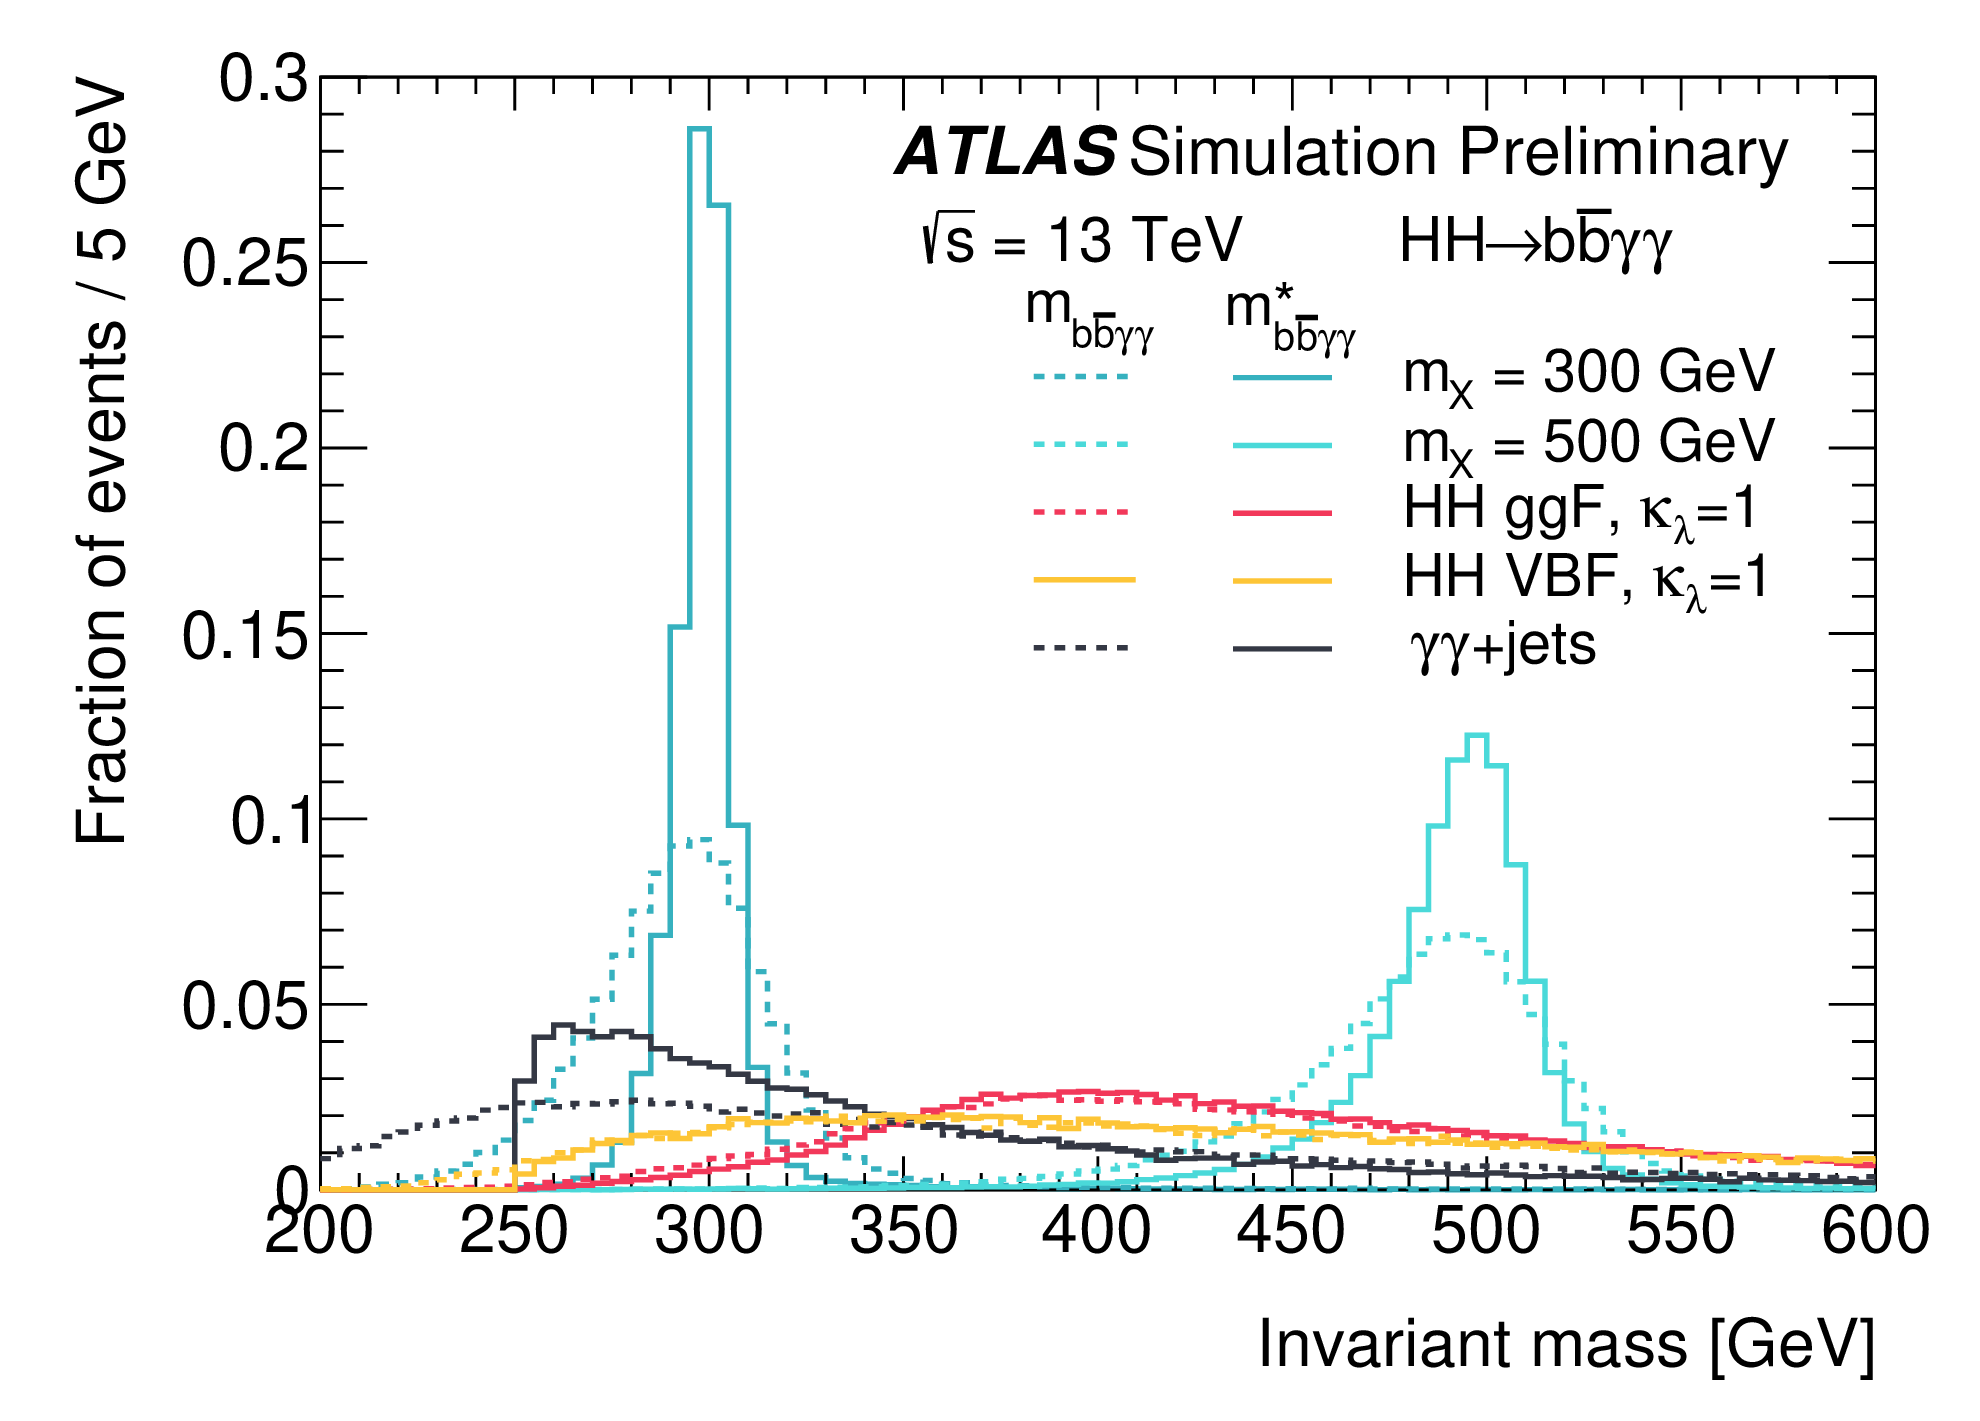
\includegraphics[width=0.5\textwidth]{BackUp/Part3/Img/mbbyy_vs_mbbyy_start.png}}
        \subfloat{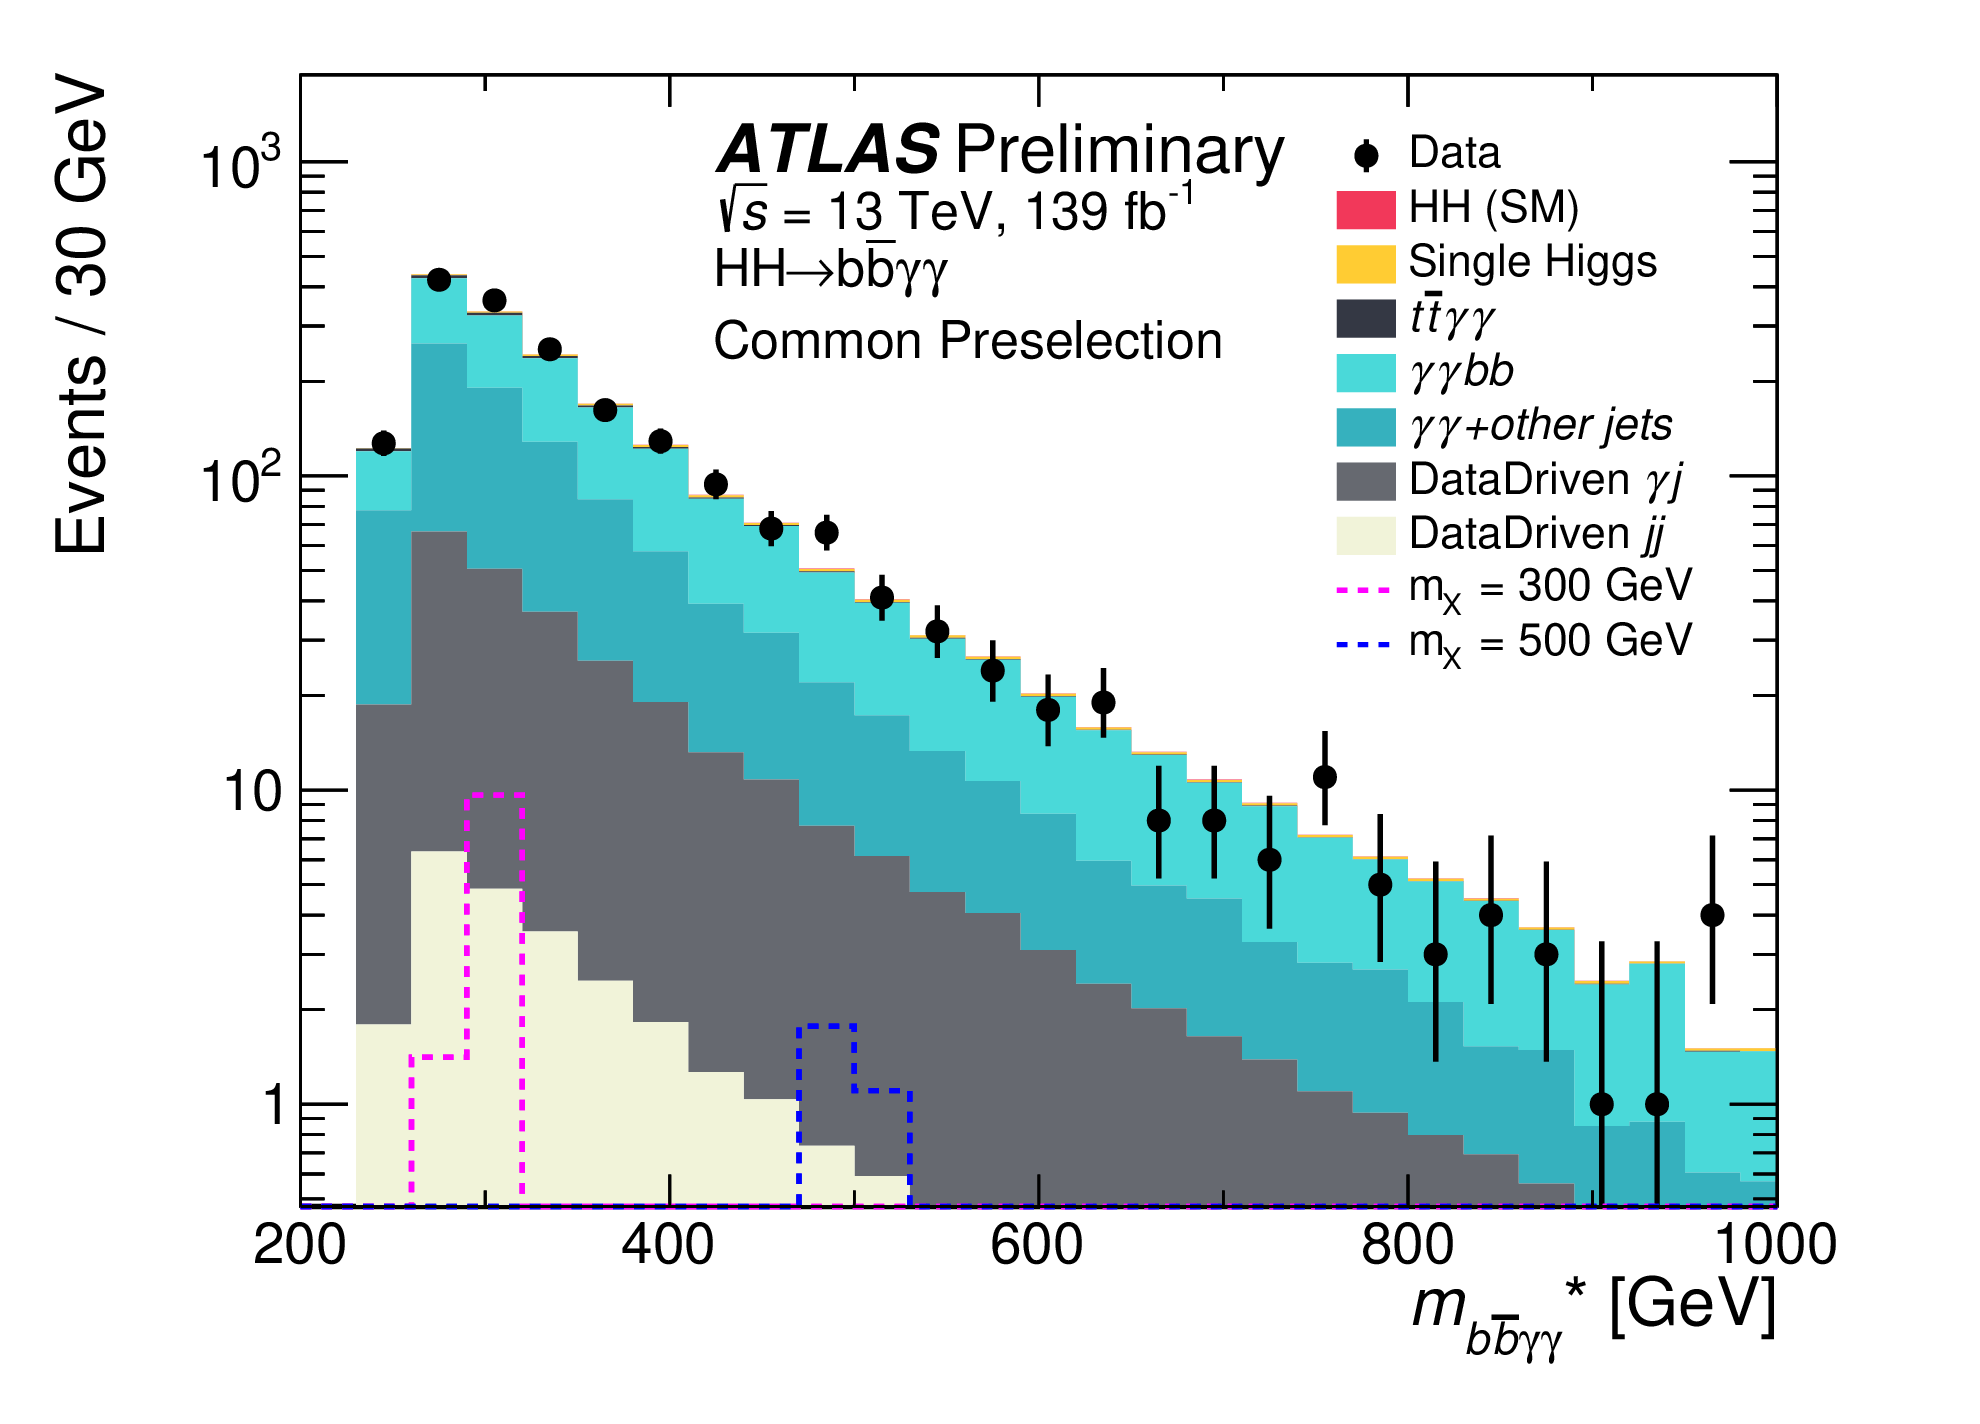
\includegraphics[width=0.5\textwidth]{BackUp/Part3/Img/mbbyy_start_data.png}}
\end{figure}
\end{frame}

\begin{frame}{$m_{b\bar{b}\gamma\gamma}^*$ distribution}
\begin{figure}
    \centering
    \subfloat{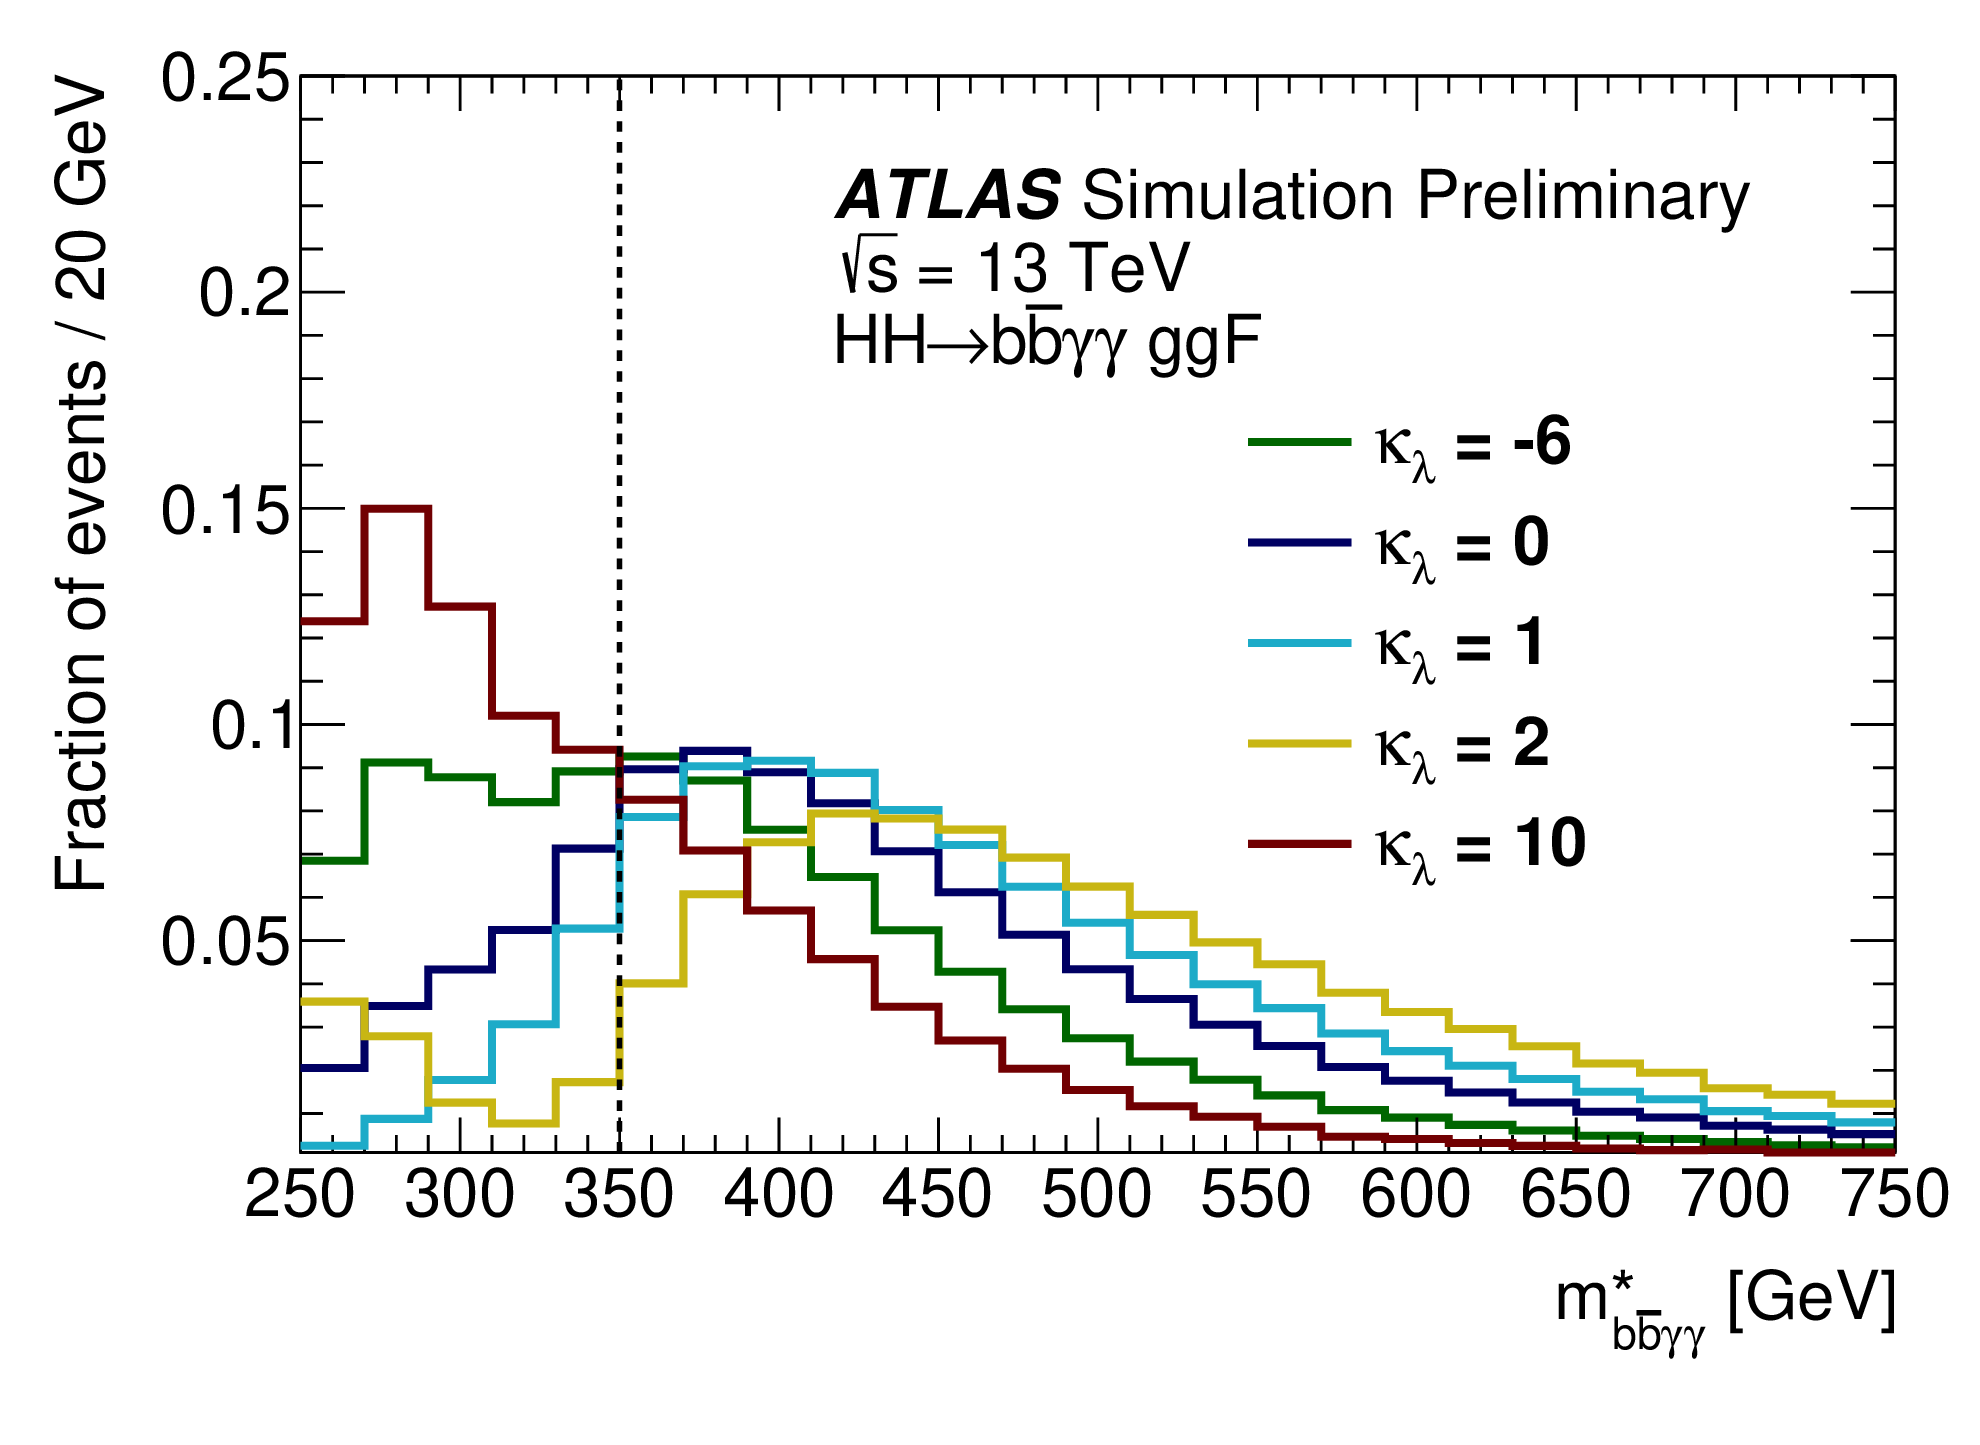
\includegraphics[width=0.5\textwidth]{BackUp/Part3/Img/ggF_mbbyy_start.png}}
    \subfloat{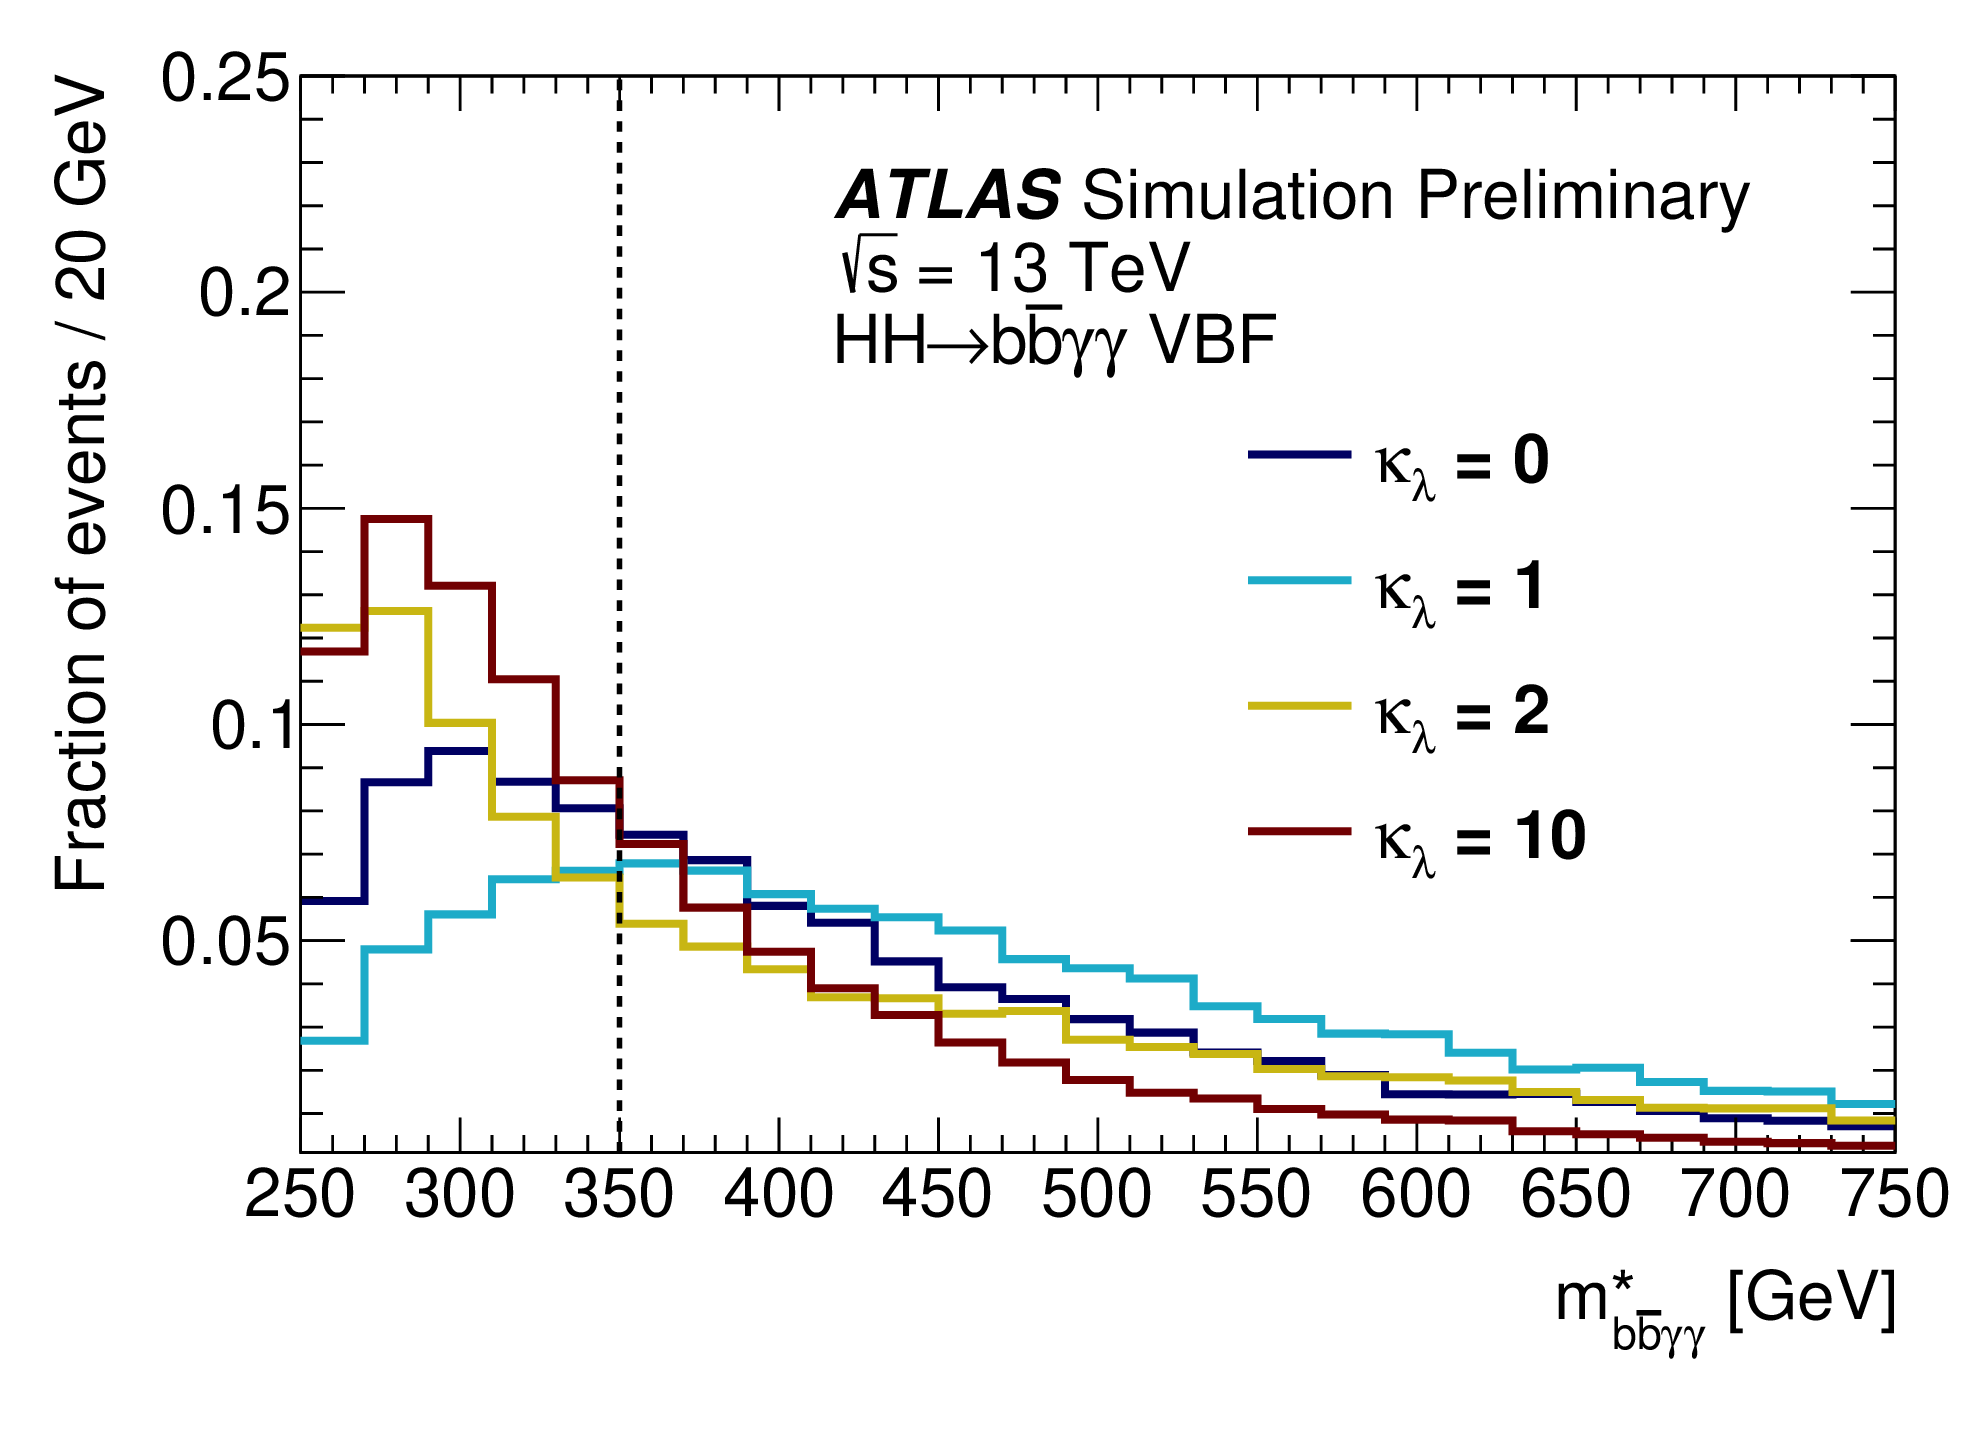
\includegraphics[width=0.5\textwidth]{BackUp/Part3/Img/VBF_mbbyy_start.png}}
\end{figure}    
\end{frame}

\begin{frame}{MVA inputs}

\begin{figure}
    \centering
    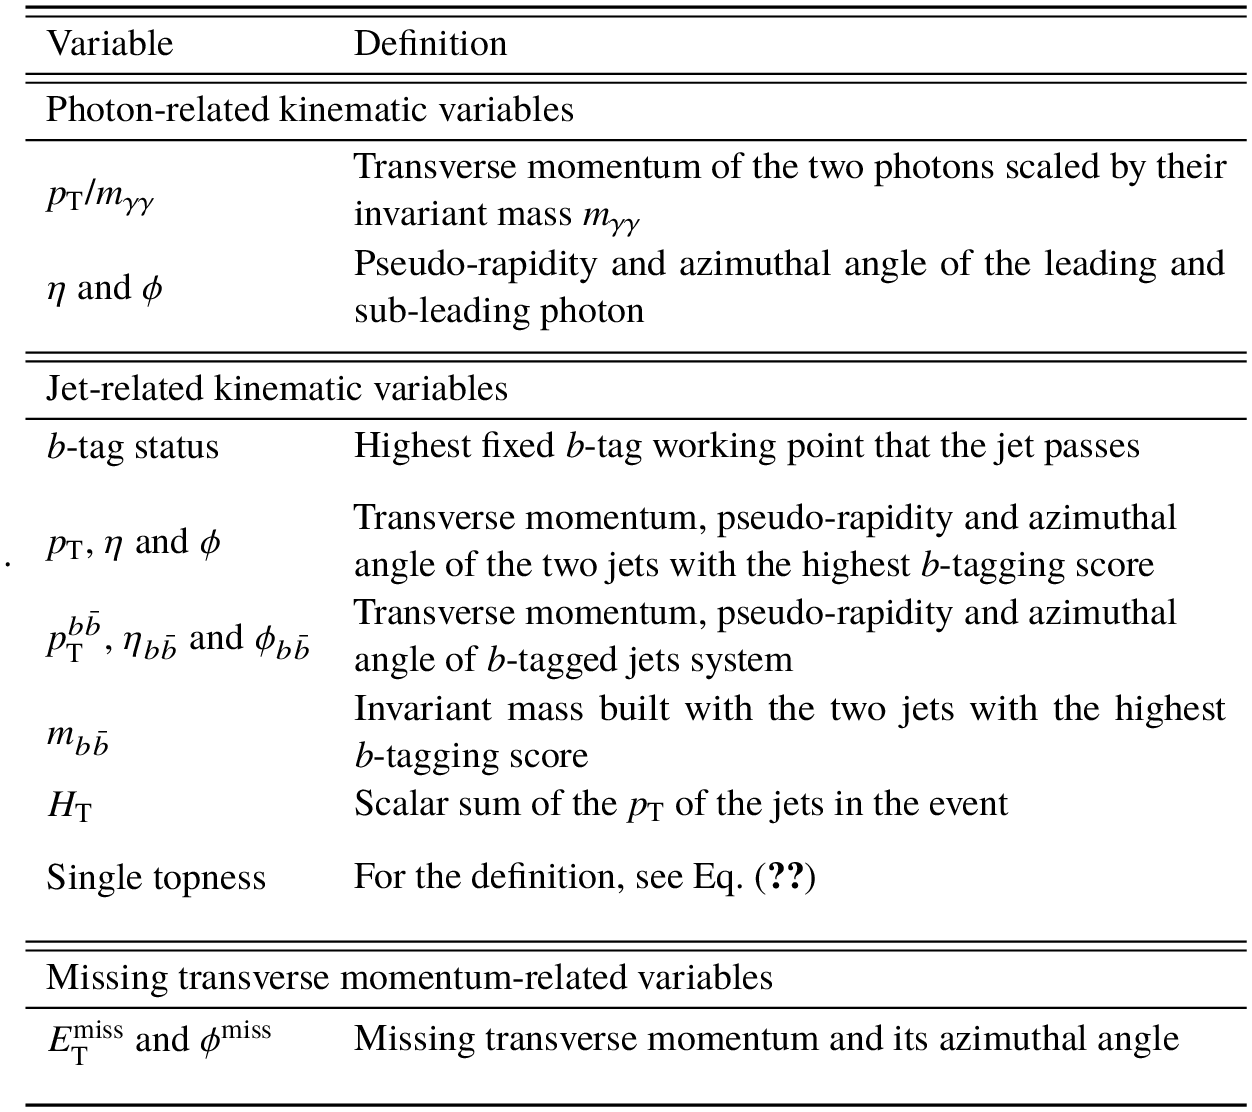
\includegraphics[width=0.5\textwidth]{BackUp/Part3/Img/BDT_inputs.png}
\end{figure}

\begin{equation*}
    \chi_{W t}=\min \sqrt{\left(\frac{m_{j_{1} j_{2}}-m_{W}}{m_{W}}\right)^{2}+\left(\frac{m_{j_{1} j_{2} j_{3}}-m_{t}}{m_{t}}\right)^{2}}
\end{equation*}
\end{frame}

\begin{frame}{Variables distributions}
\begin{columns}
\column{0.5\textwidth}
\begin{figure}
    \centering
    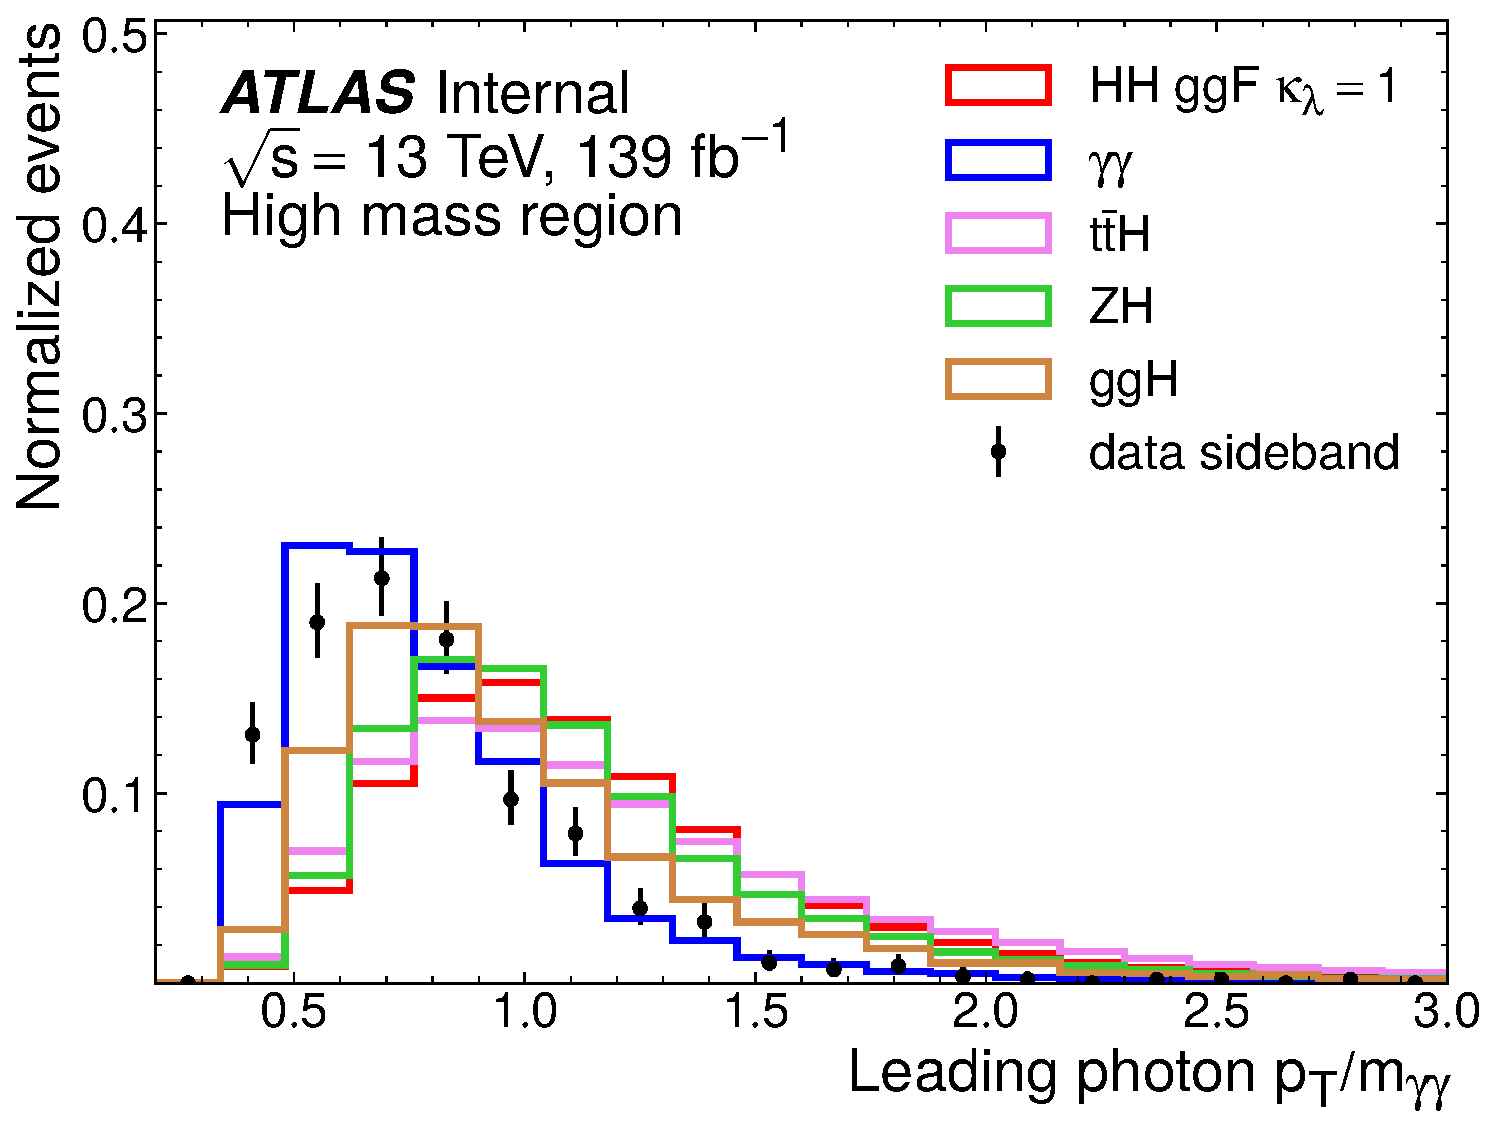
\includegraphics[width=1.\textwidth]{BackUp/Part3/Img/var_SM_rel_photon1_pt.pdf}
\end{figure}
\column{0.5\textwidth}
\begin{figure}
    \centering
    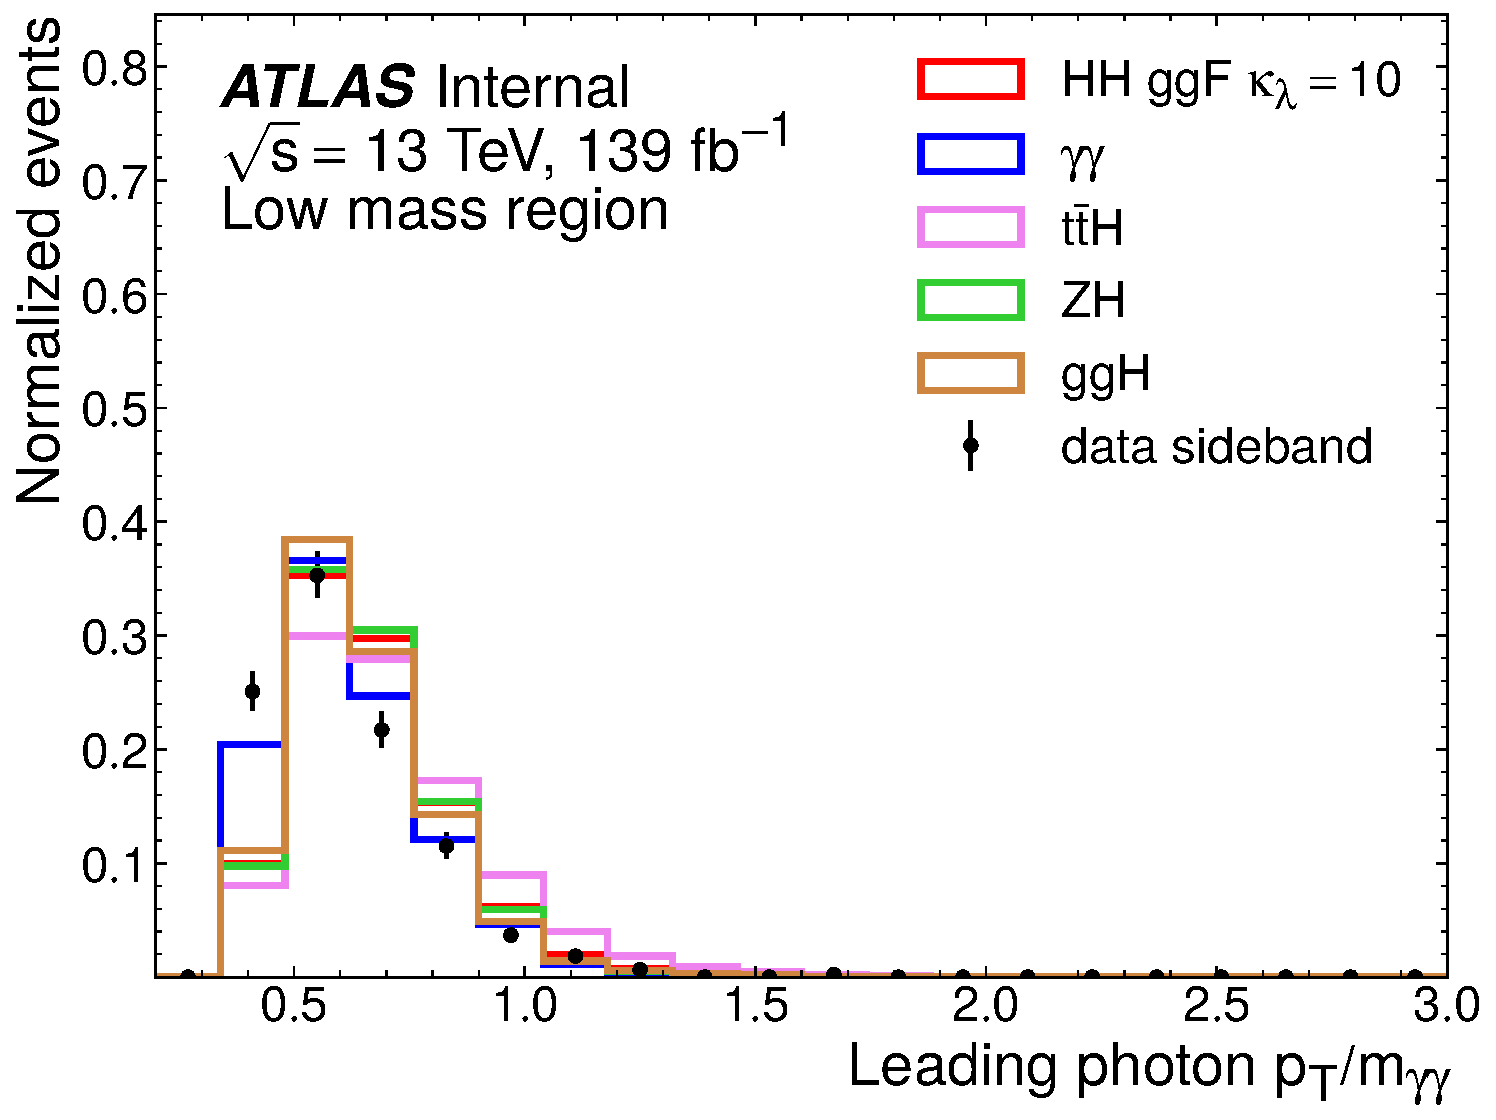
\includegraphics[width=1.\textwidth]{BackUp/Part3/Img/var_BSM_rel_photon1_pt.pdf}
\end{figure}
\end{columns}
\end{frame}

\begin{frame}{Variables distributions}
\begin{columns}
\column{0.5\textwidth}
\begin{figure}
    \centering
    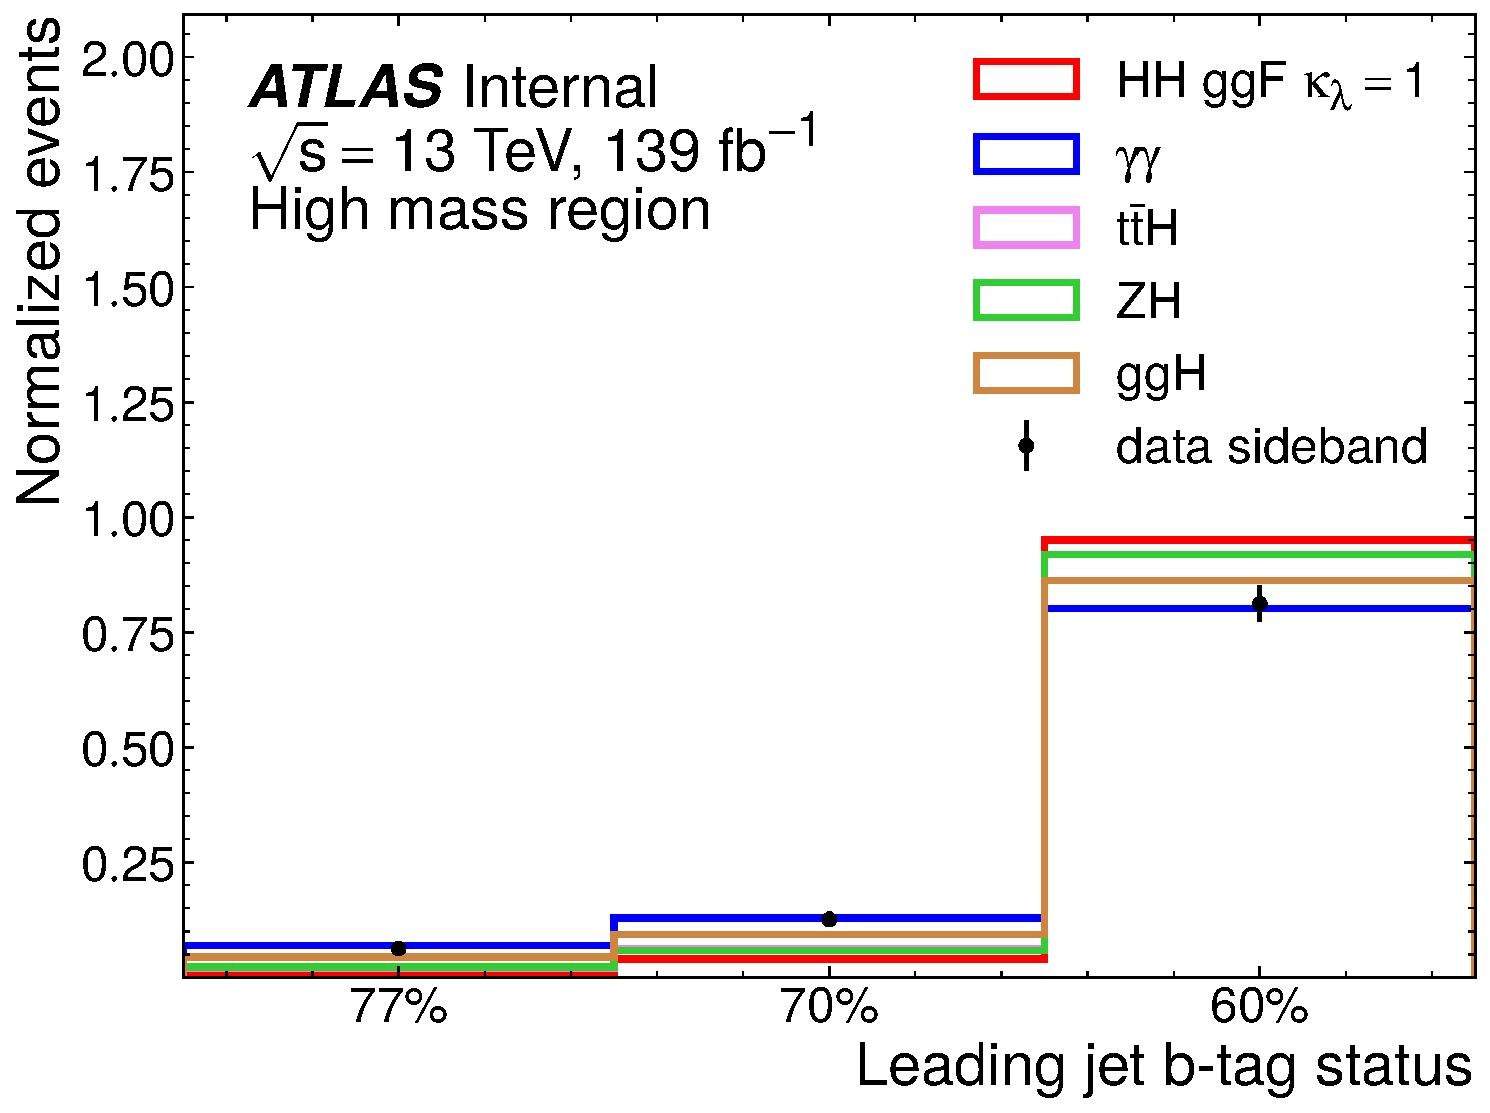
\includegraphics[width=1.\textwidth]{BackUp/Part3/Img/var_SM_jet1_btag.pdf}
\end{figure}
\column{0.5\textwidth}
\begin{figure}
    \centering
    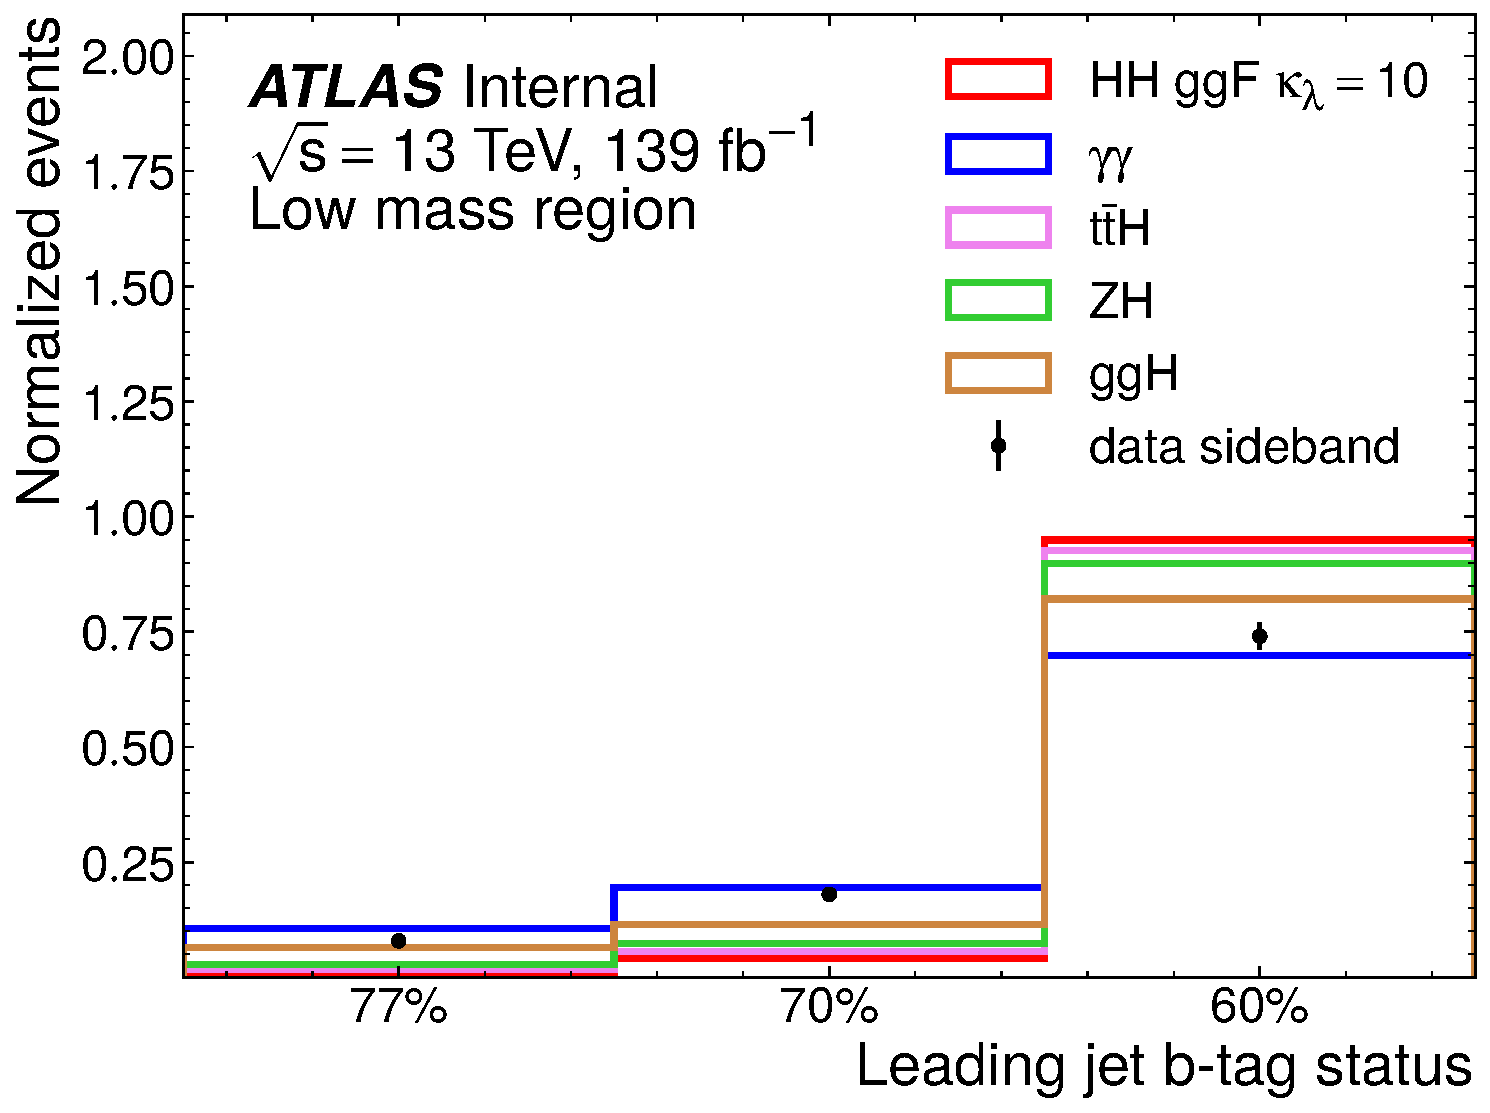
\includegraphics[width=1.\textwidth]{BackUp/Part3/Img/var_BSM_jet1_btag.pdf}
\end{figure}
\end{columns}
\end{frame}

\begin{frame}{Variables distributions}
\begin{columns}
\column{0.5\textwidth}
\begin{figure}
    \centering
    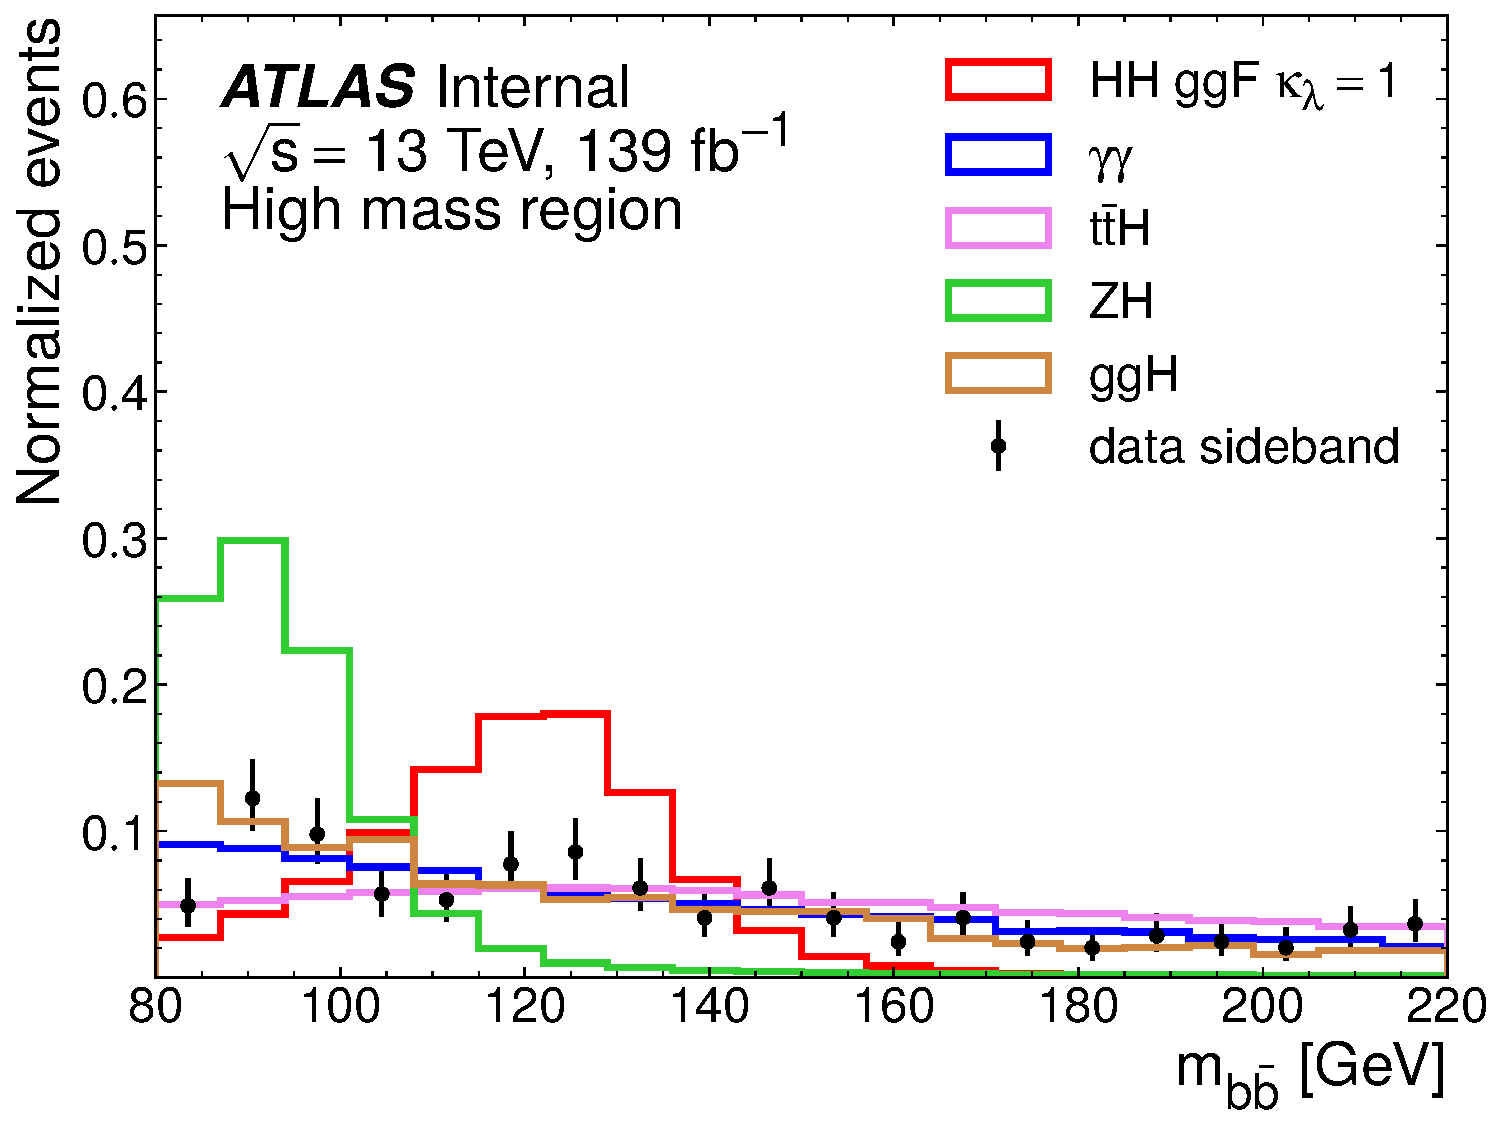
\includegraphics[width=1.\textwidth]{BackUp/Part3/Img/var_SM_bb_M.pdf}
\end{figure}
\column{0.5\textwidth}
\begin{figure}
    \centering
    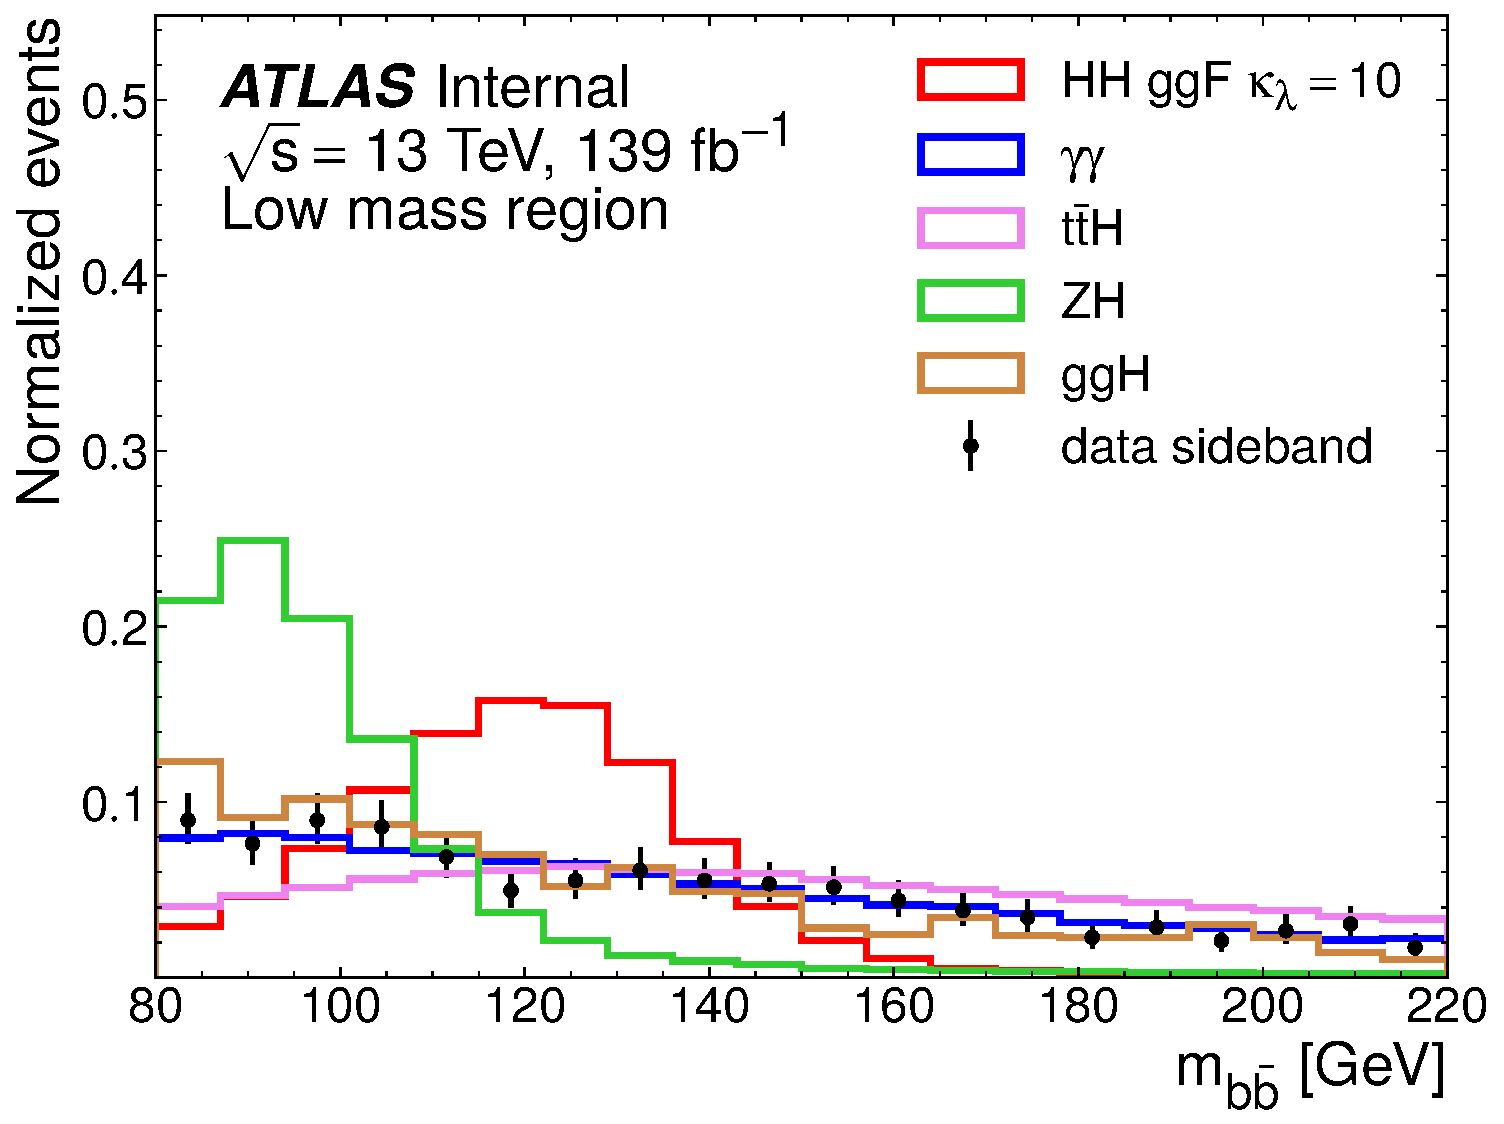
\includegraphics[width=1.\textwidth]{BackUp/Part3/Img/var_BSM_bb_M.pdf}
\end{figure}
\end{columns}
\end{frame}

\begin{frame}{Variables distributions}
\begin{columns}
\column{0.5\textwidth}
\begin{figure}
    \centering
    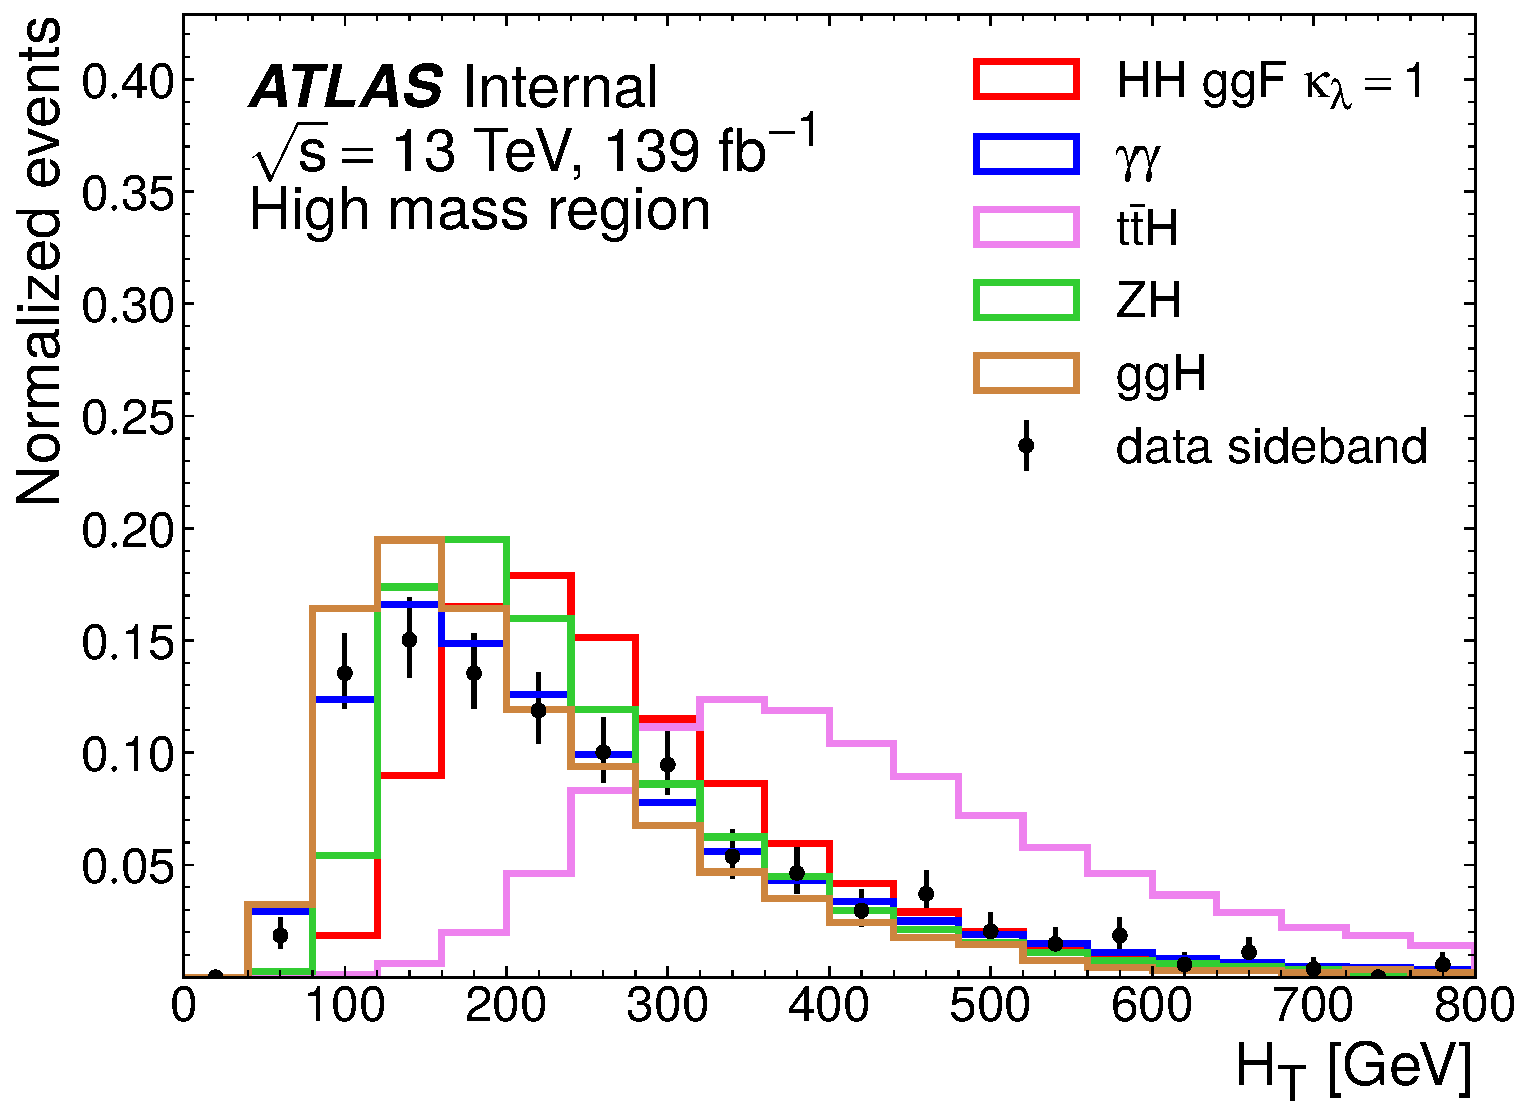
\includegraphics[width=1.\textwidth]{BackUp/Part3/Img/var_SM_HT.pdf}
\end{figure}
\column{0.5\textwidth}
\begin{figure}
    \centering
    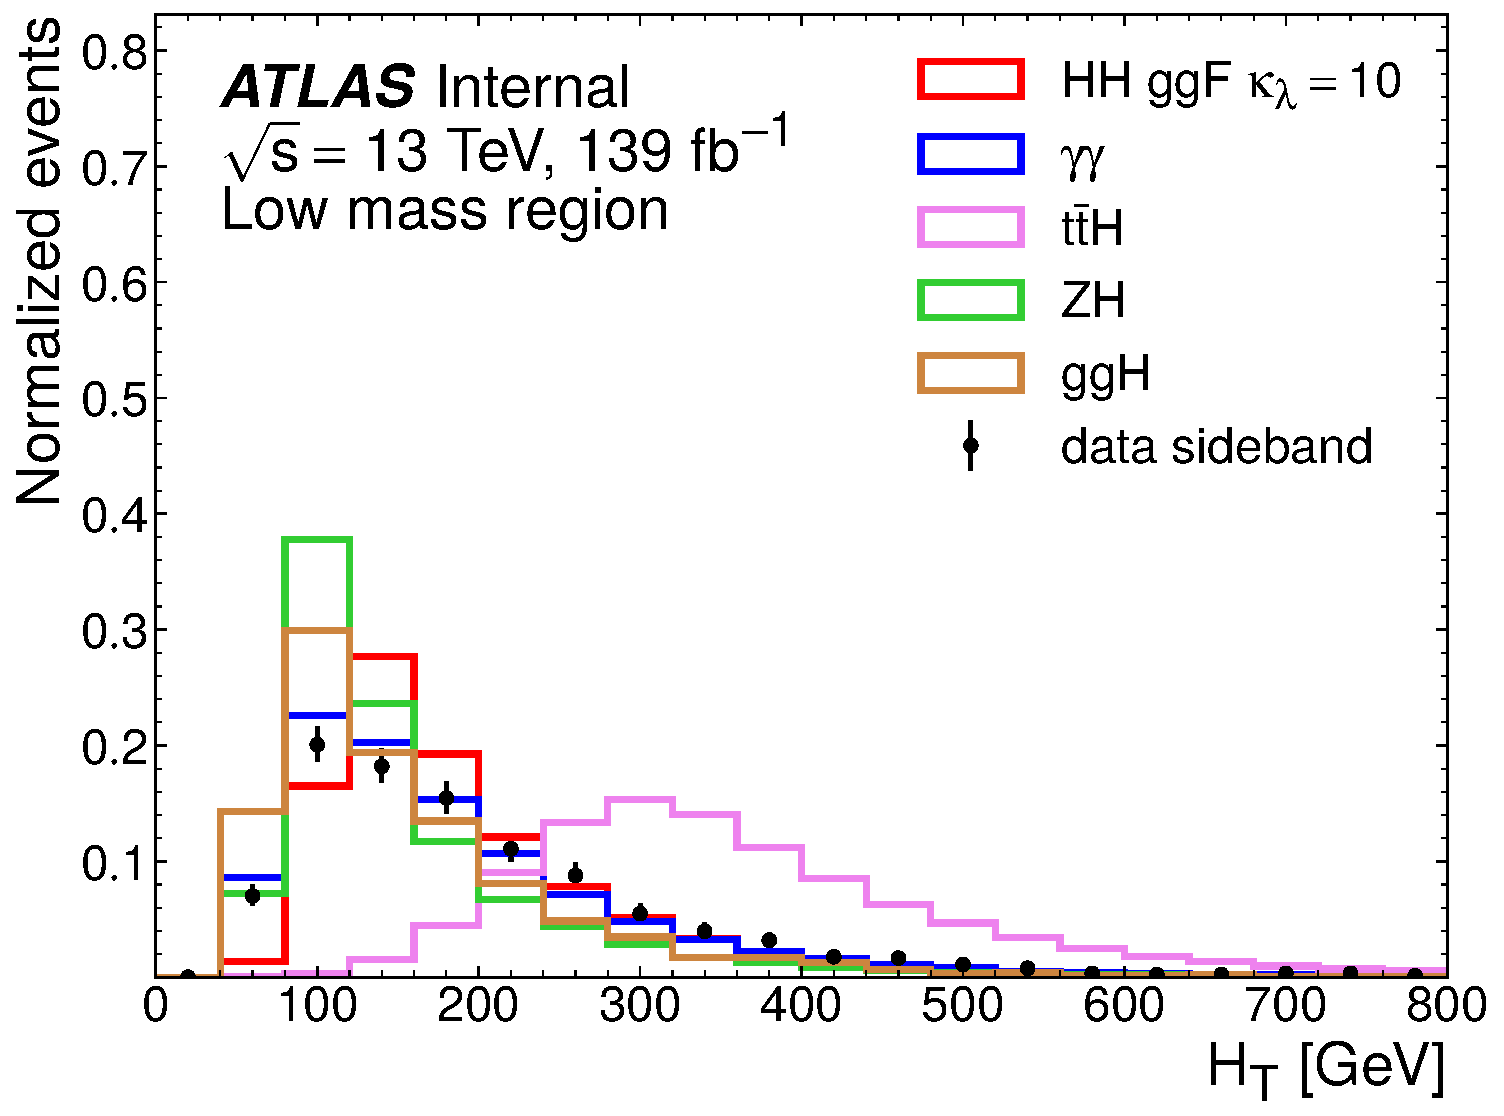
\includegraphics[width=1.\textwidth]{BackUp/Part3/Img/var_BSM_HT.pdf}
\end{figure}
\end{columns}
\end{frame}

\begin{frame}{Variables distributions}
\begin{columns}
\column{0.5\textwidth}
\begin{figure}
    \centering
    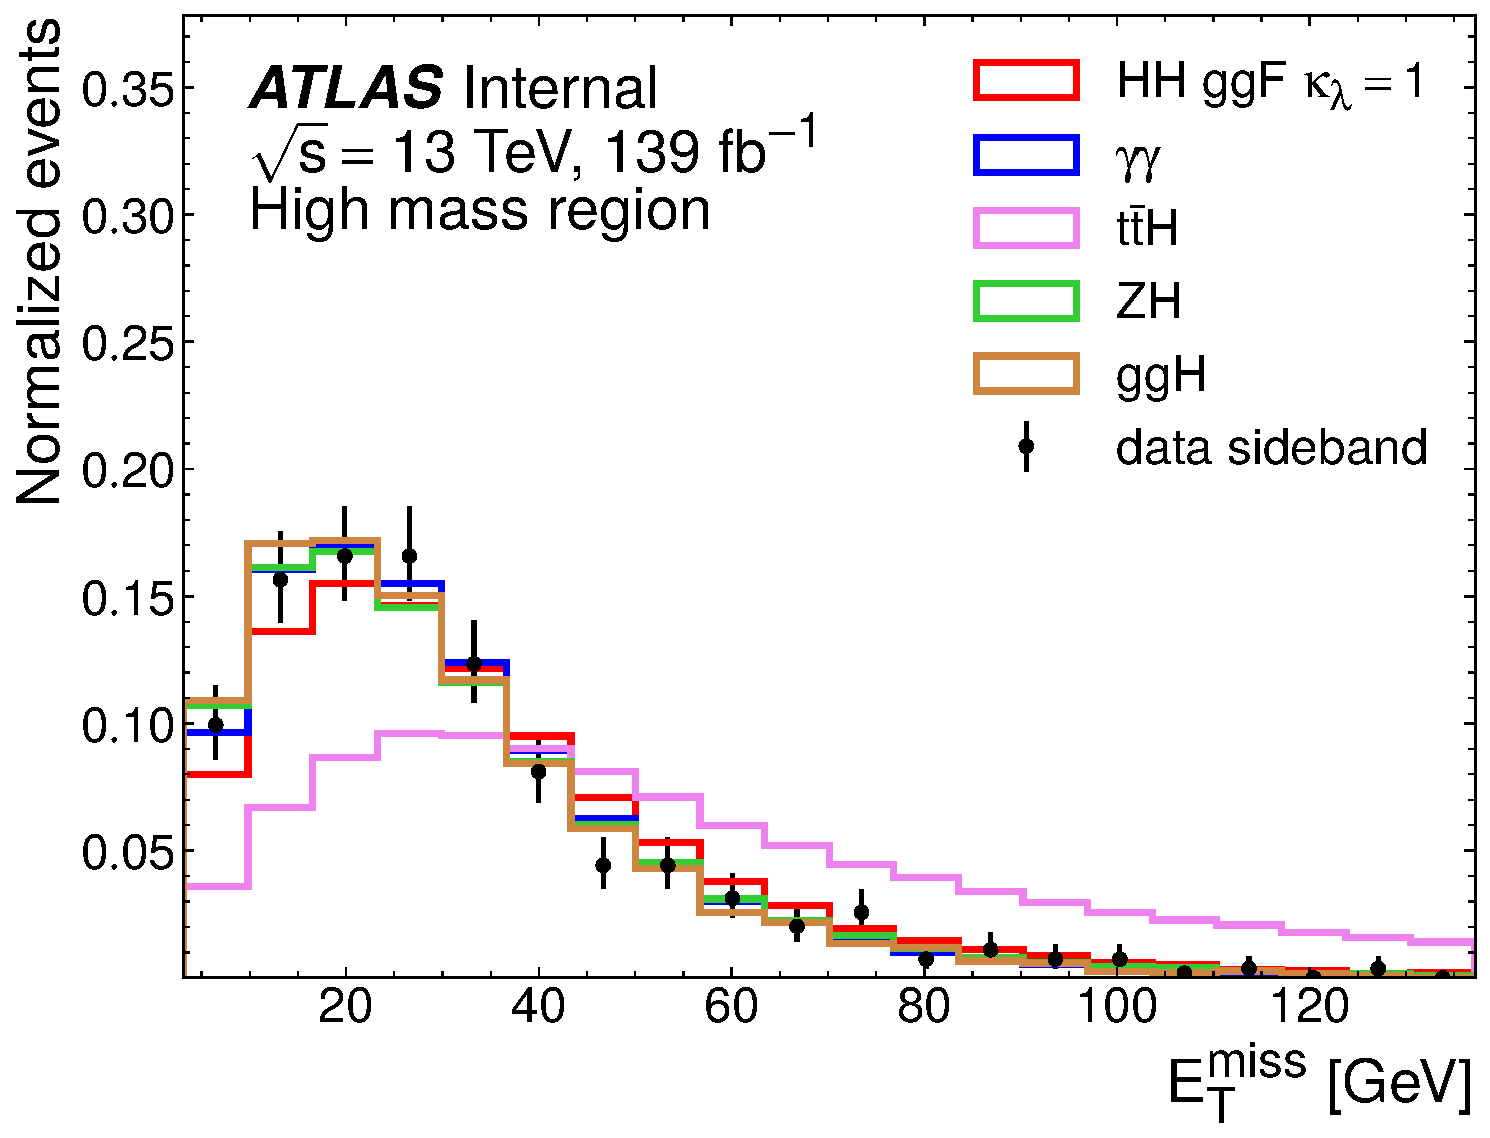
\includegraphics[width=1.\textwidth]{BackUp/Part3/Img/var_SM_met_pt.pdf}
\end{figure}
\column{0.5\textwidth}
\begin{figure}
    \centering
    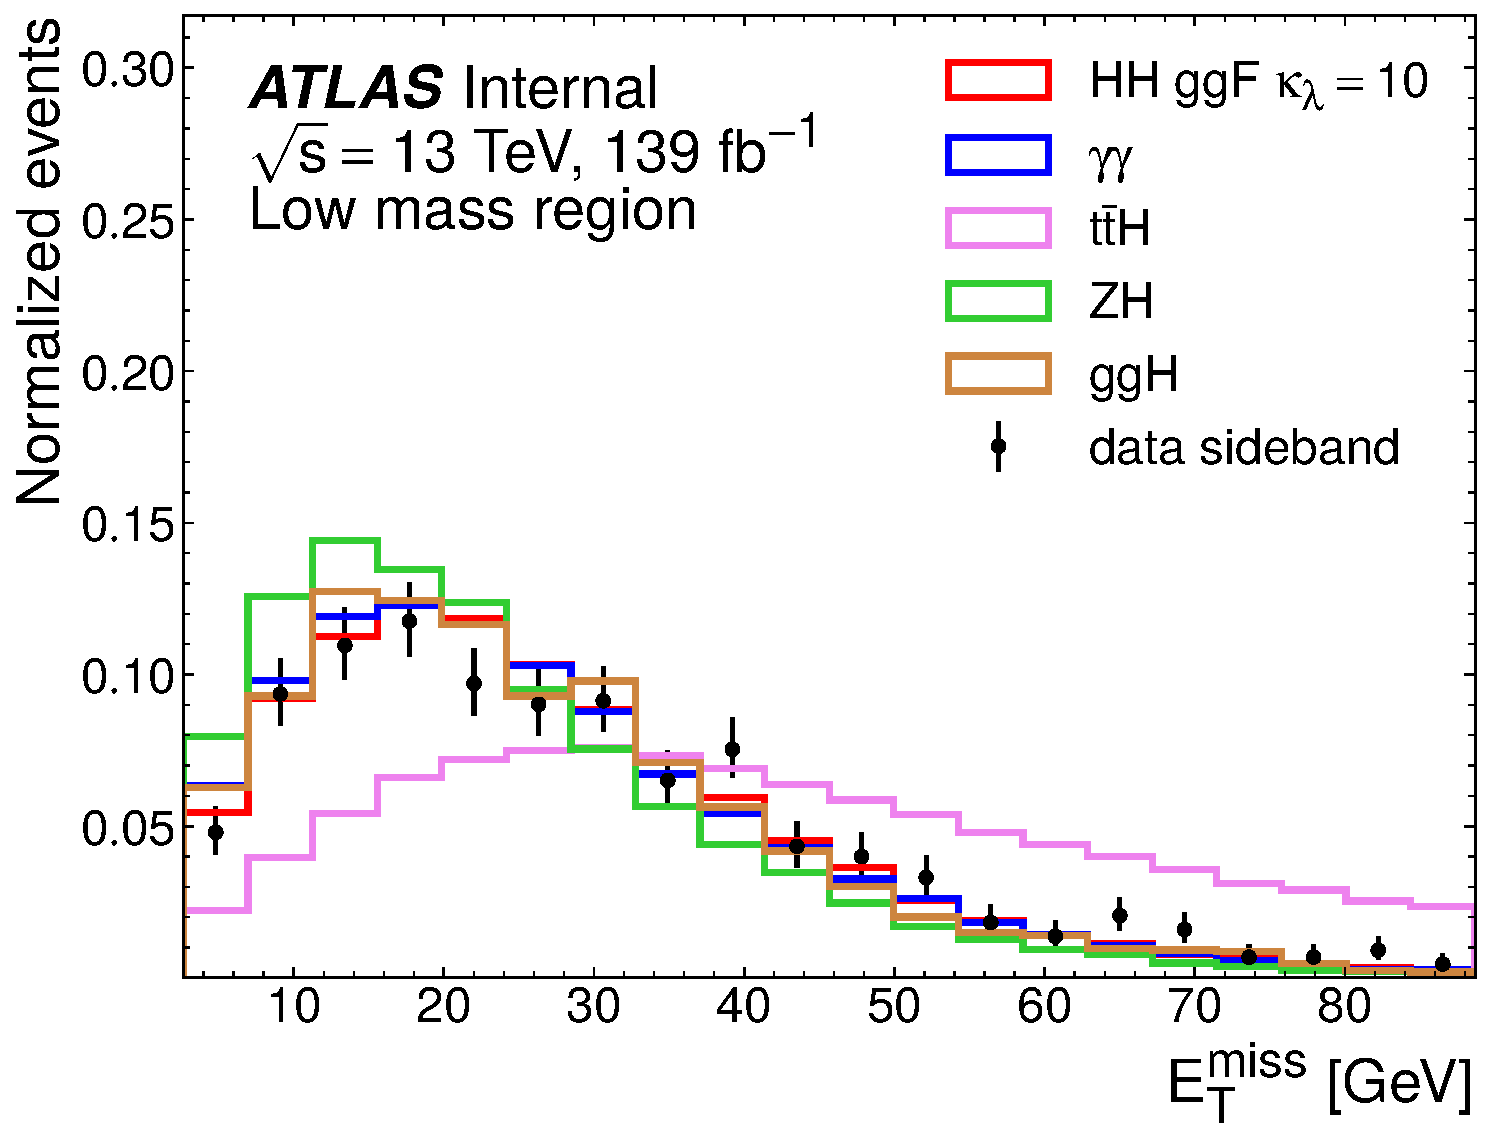
\includegraphics[width=1.\textwidth]{BackUp/Part3/Img/var_BSM_met_pt.pdf}
\end{figure}
\end{columns}
\end{frame}

\begin{frame}{Variables distributions}
\begin{columns}
\column{0.5\textwidth}
\begin{figure}
    \centering
    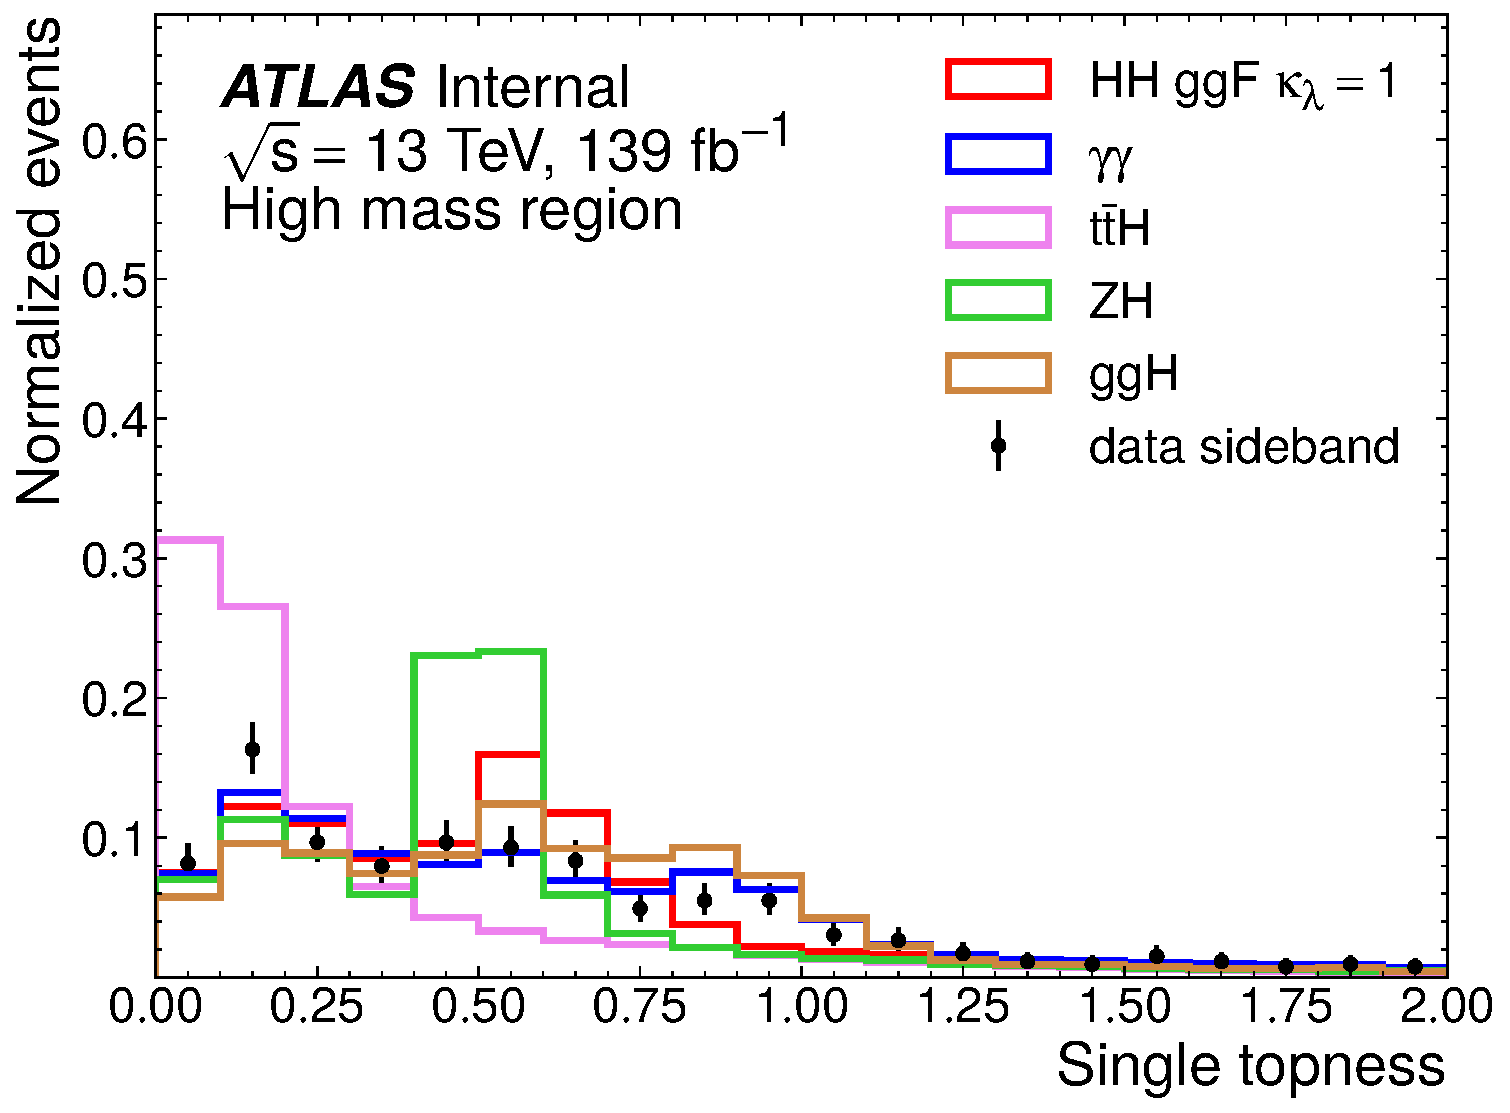
\includegraphics[width=1.\textwidth]{BackUp/Part3/Img/var_SM_single_topness.pdf}
\end{figure}
\column{0.5\textwidth}
\begin{figure}
    \centering
    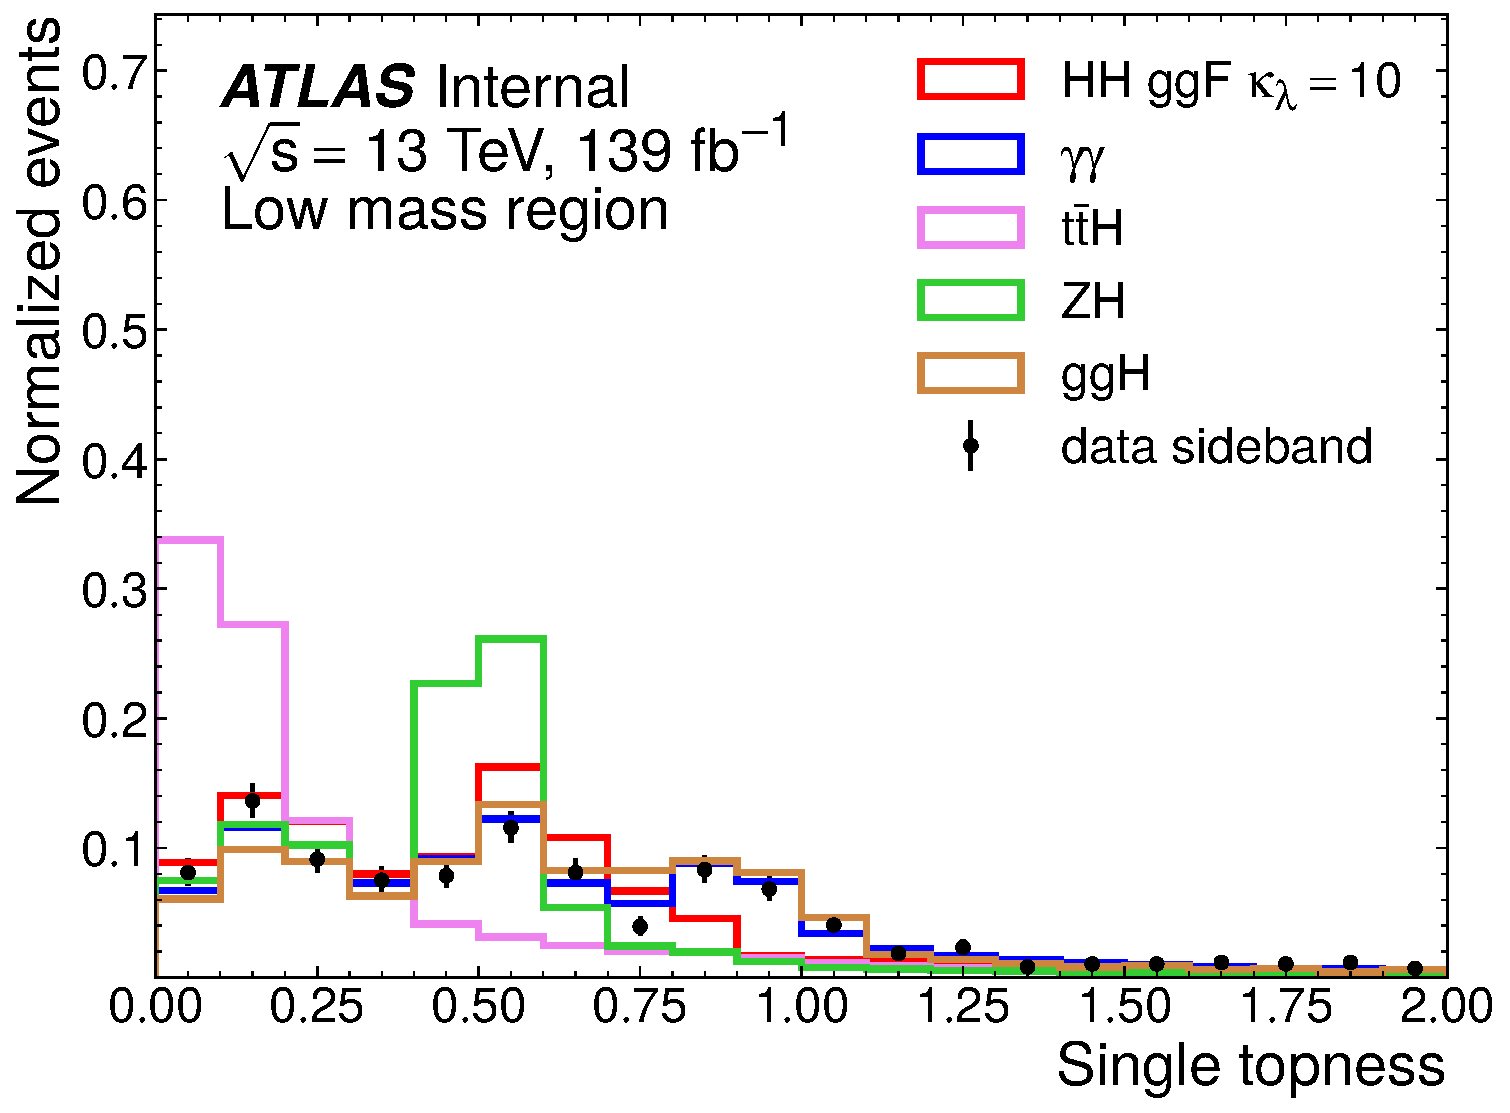
\includegraphics[width=1.\textwidth]{BackUp/Part3/Img/var_BSM_single_topness.pdf}
\end{figure}
\end{columns}
\end{frame}
\begin{frame}{DNN loss function}
\begin{figure}
    \centering
    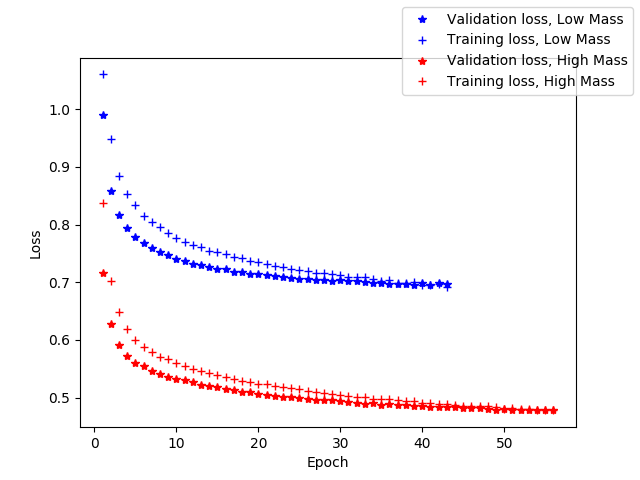
\includegraphics[width=0.7\textwidth]{BackUp/Part3/Img/Loss_DNN.png}
\end{figure}    
\end{frame}

\begin{frame}{DNN confusion matrix}
\begin{figure}
    \centering
    \subfloat{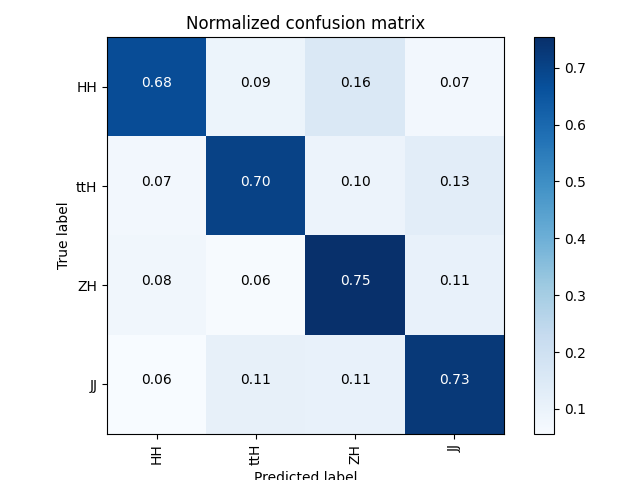
\includegraphics[width=0.5\textwidth]{BackUp/Part3/Img/cm_SM.png}}
    \subfloat{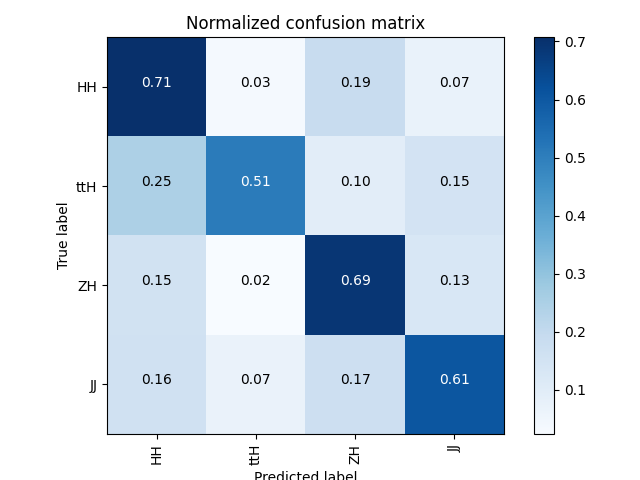
\includegraphics[width=0.5\textwidth]{BackUp/Part3/Img/cm_BSM.png}}
\end{figure}
JJ = continuum $\gamma\gamma$+jets
\end{frame}

\begin{frame}{$d_{HH}$ distribution}
\begin{figure}
    \centering
    \subfloat{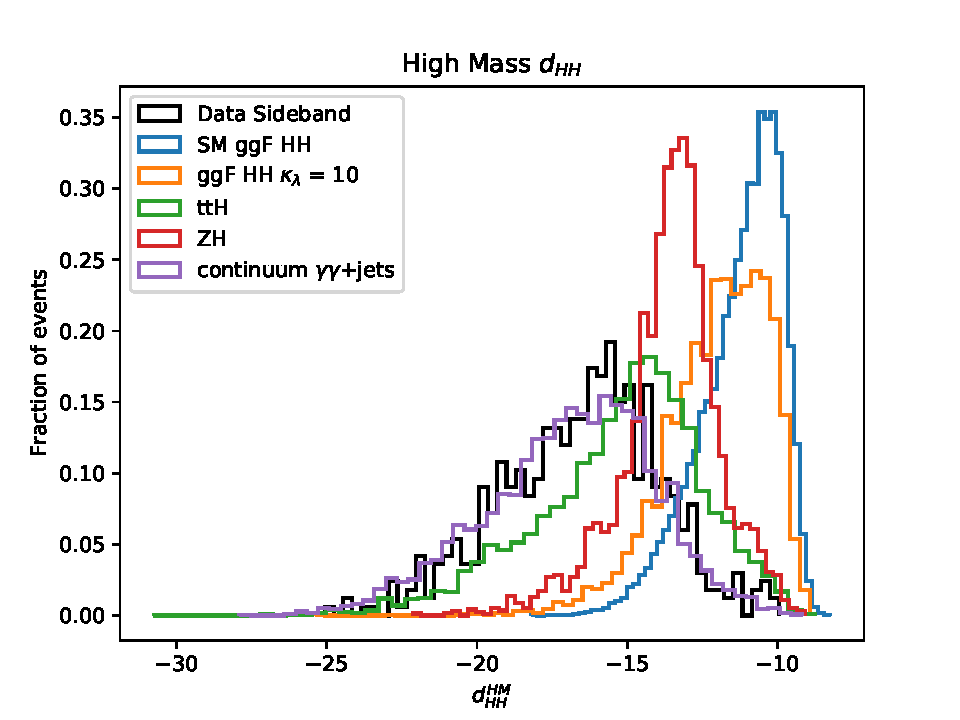
\includegraphics[width=0.5\textwidth]{BackUp/Part3/Img/dHH_SM.pdf}}
    \subfloat{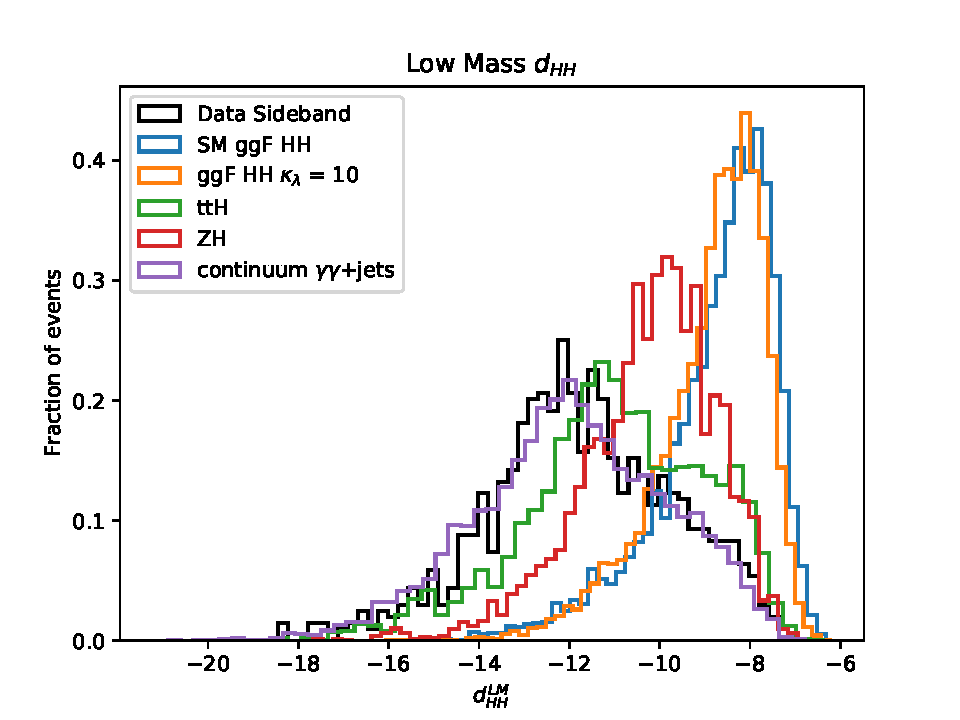
\includegraphics[width=0.5\textwidth]{BackUp/Part3/Img/dHH_BSM.pdf}}
\end{figure}    
\end{frame}

\begin{frame}{DNN significance breakdwon}
\begin{table}[htbp]
    \centering
    \begin{tabular}{lcc}
        \hline\hline
        Categories & SM ggF HH & BSM $\kappa_\lambda$=10 ggF HH \\
        \hline
        High mass, High $d_{HH}$ & 0.53 & 2.45 \\
        High mass, Low $d_{HH}$ & 0.11 & 0.94 \\
        Low mass, High $d_{HH}$ & 0.03 & 2.21 \\
        Low mass, Low $d_{HH}$ & 0.01 & 0.54 \\
        \hline
        Combined & 0.54$\sigma$ & 3.47$\sigma$ \\
        \hline
        \hline
    \end{tabular}
\end{table}
\end{frame}

\begin{frame}{BDT categories}
\begin{figure}
    \centering
    \subfloat{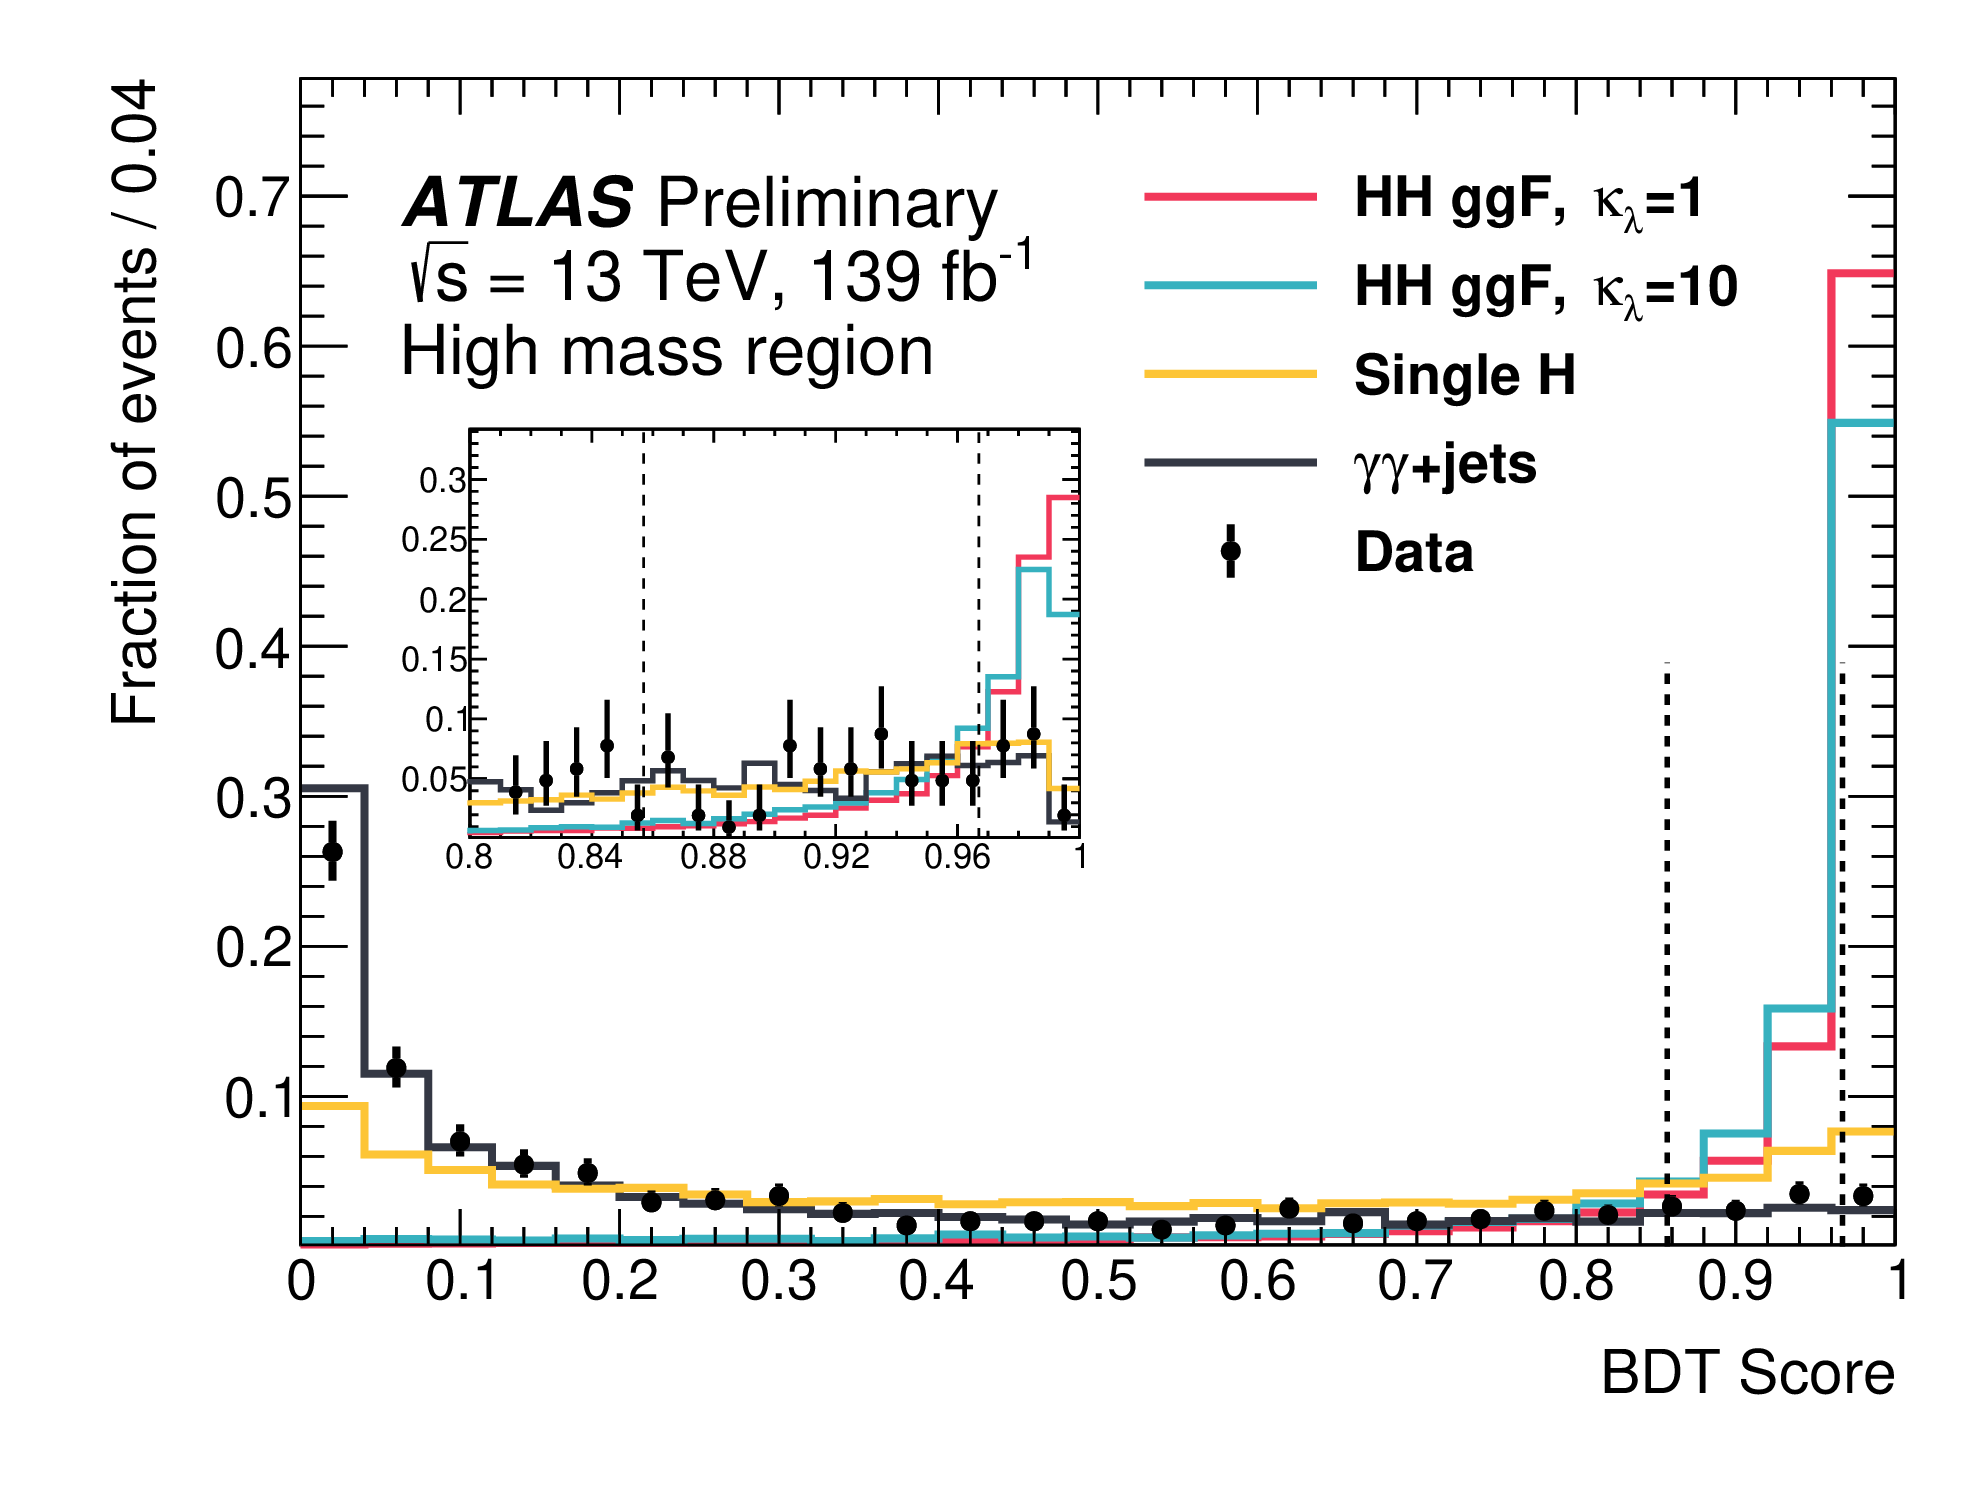
\includegraphics[width=0.5\textwidth]{BackUp/Part3/Img/BDT_SM.png}}
    \subfloat{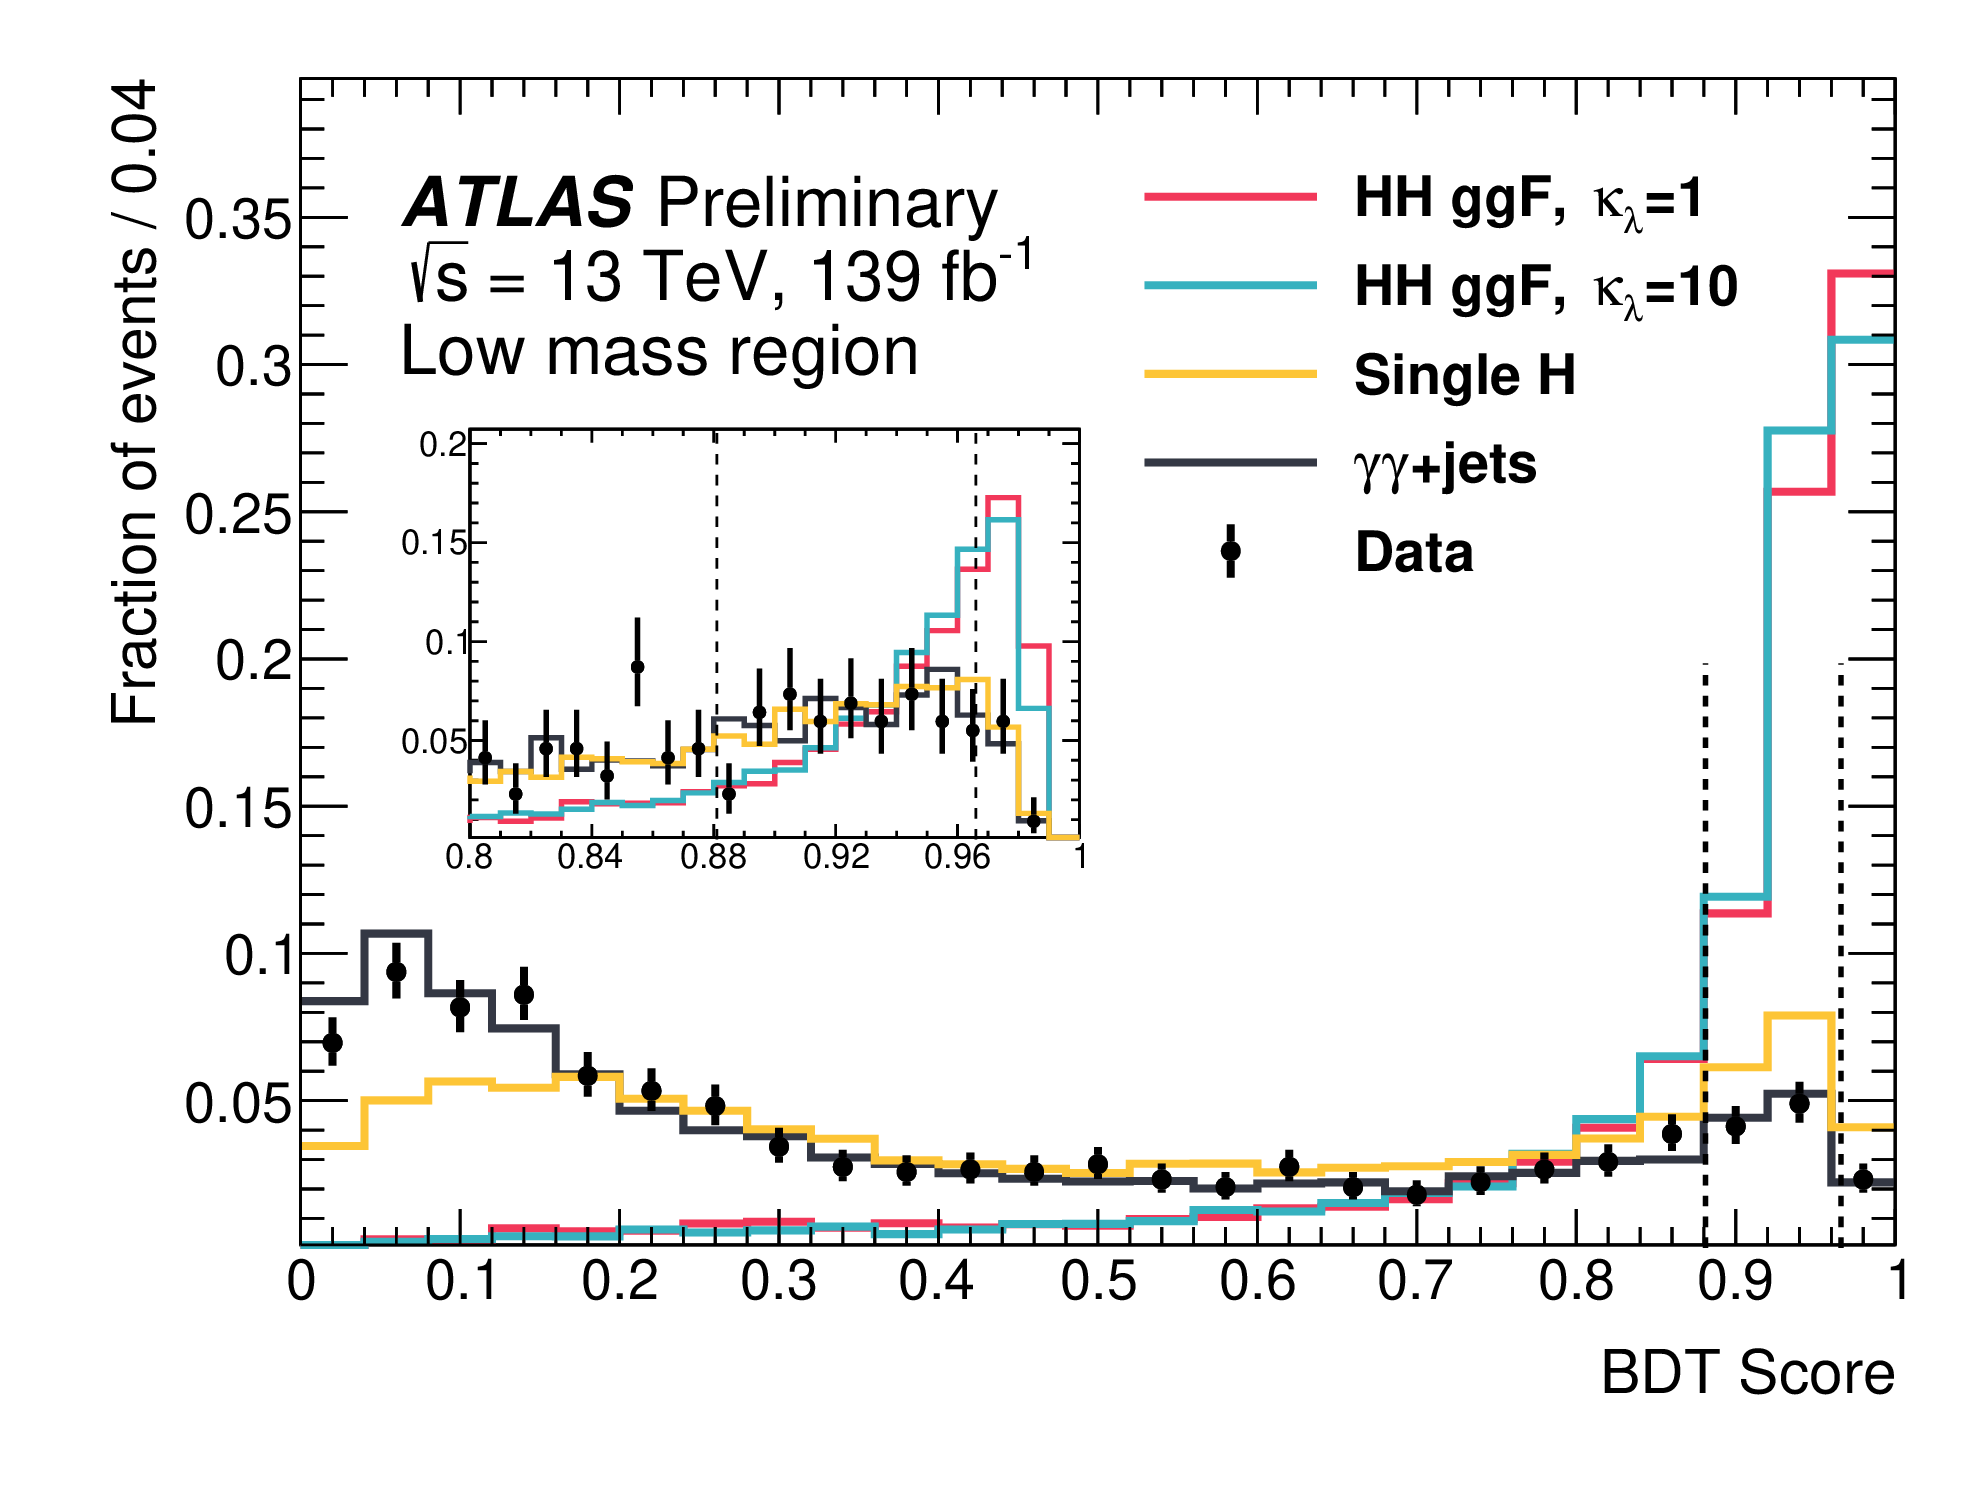
\includegraphics[width=0.5\textwidth]{BackUp/Part3/Img/BDT_BSM.png}}\\
    \subfloat{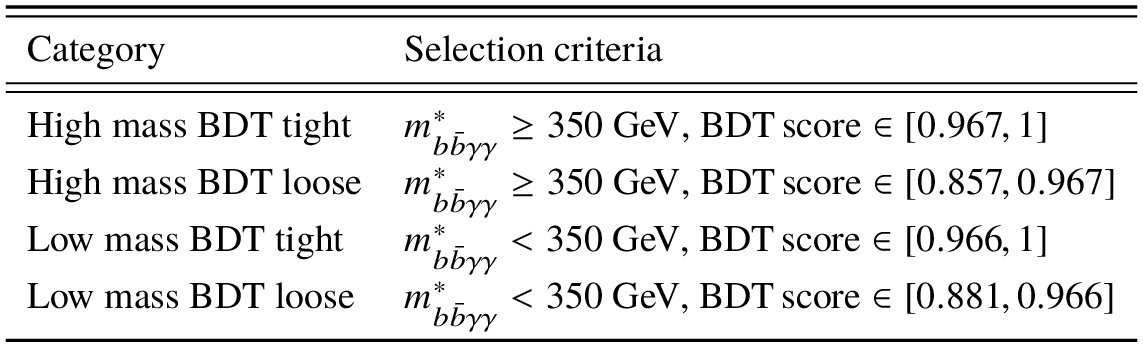
\includegraphics[width=0.45\textwidth]{BackUp/Part3/Img/BDT_cuts.png}}
\end{figure}
\end{frame}

\begin{frame}{Analysis categories}
\begin{figure}
    \centering
    \subfloat{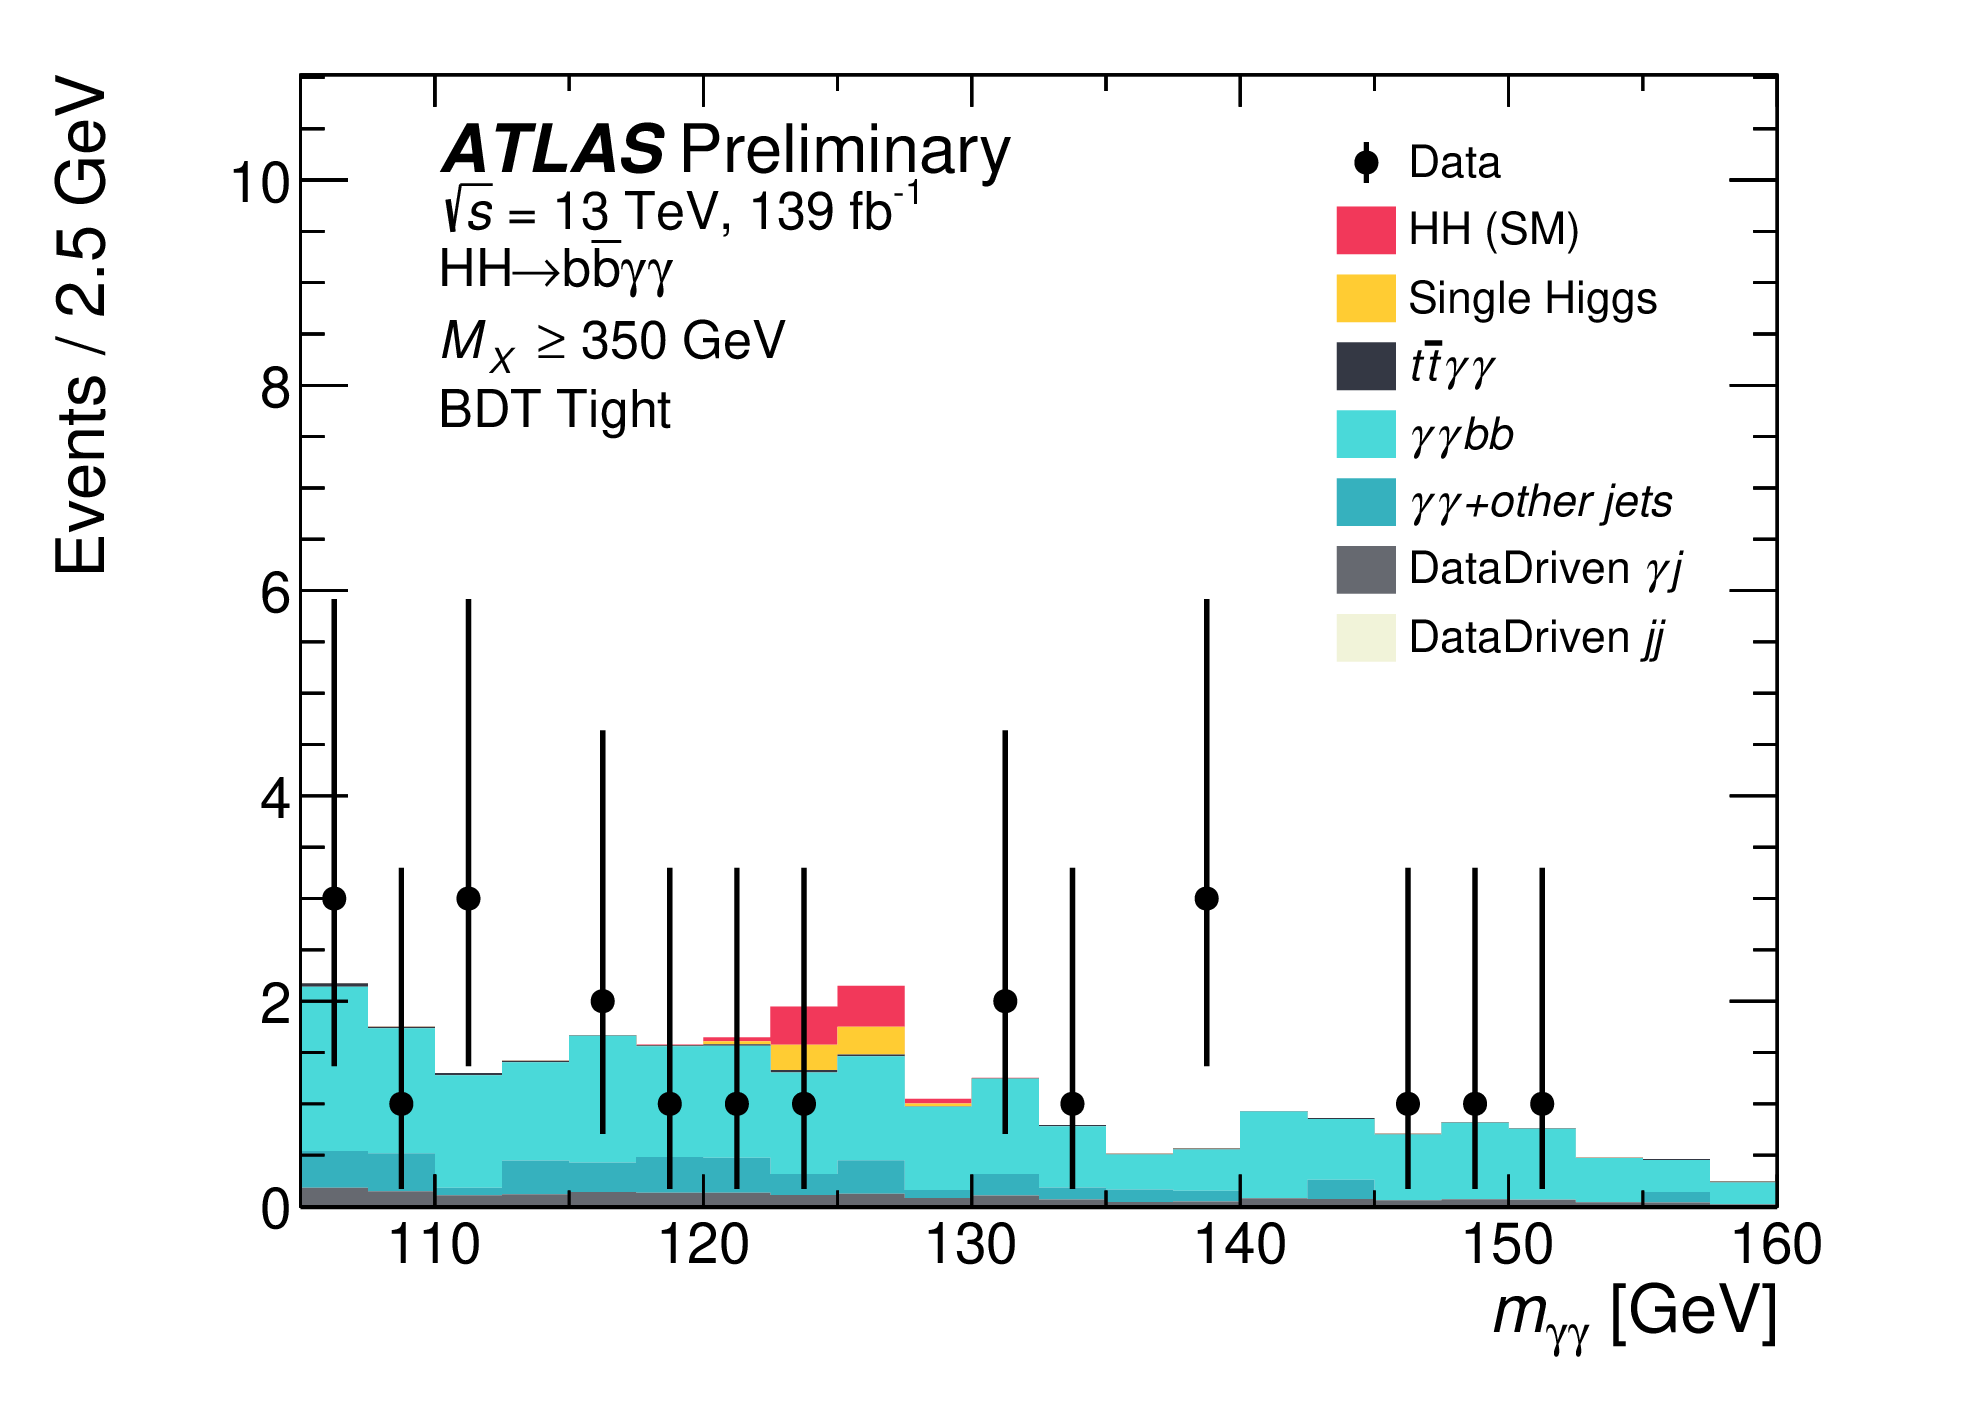
\includegraphics[width=0.35\textwidth]{BackUp/Part3/Img/High_mass_BDT_tight_data.png}}
    \subfloat{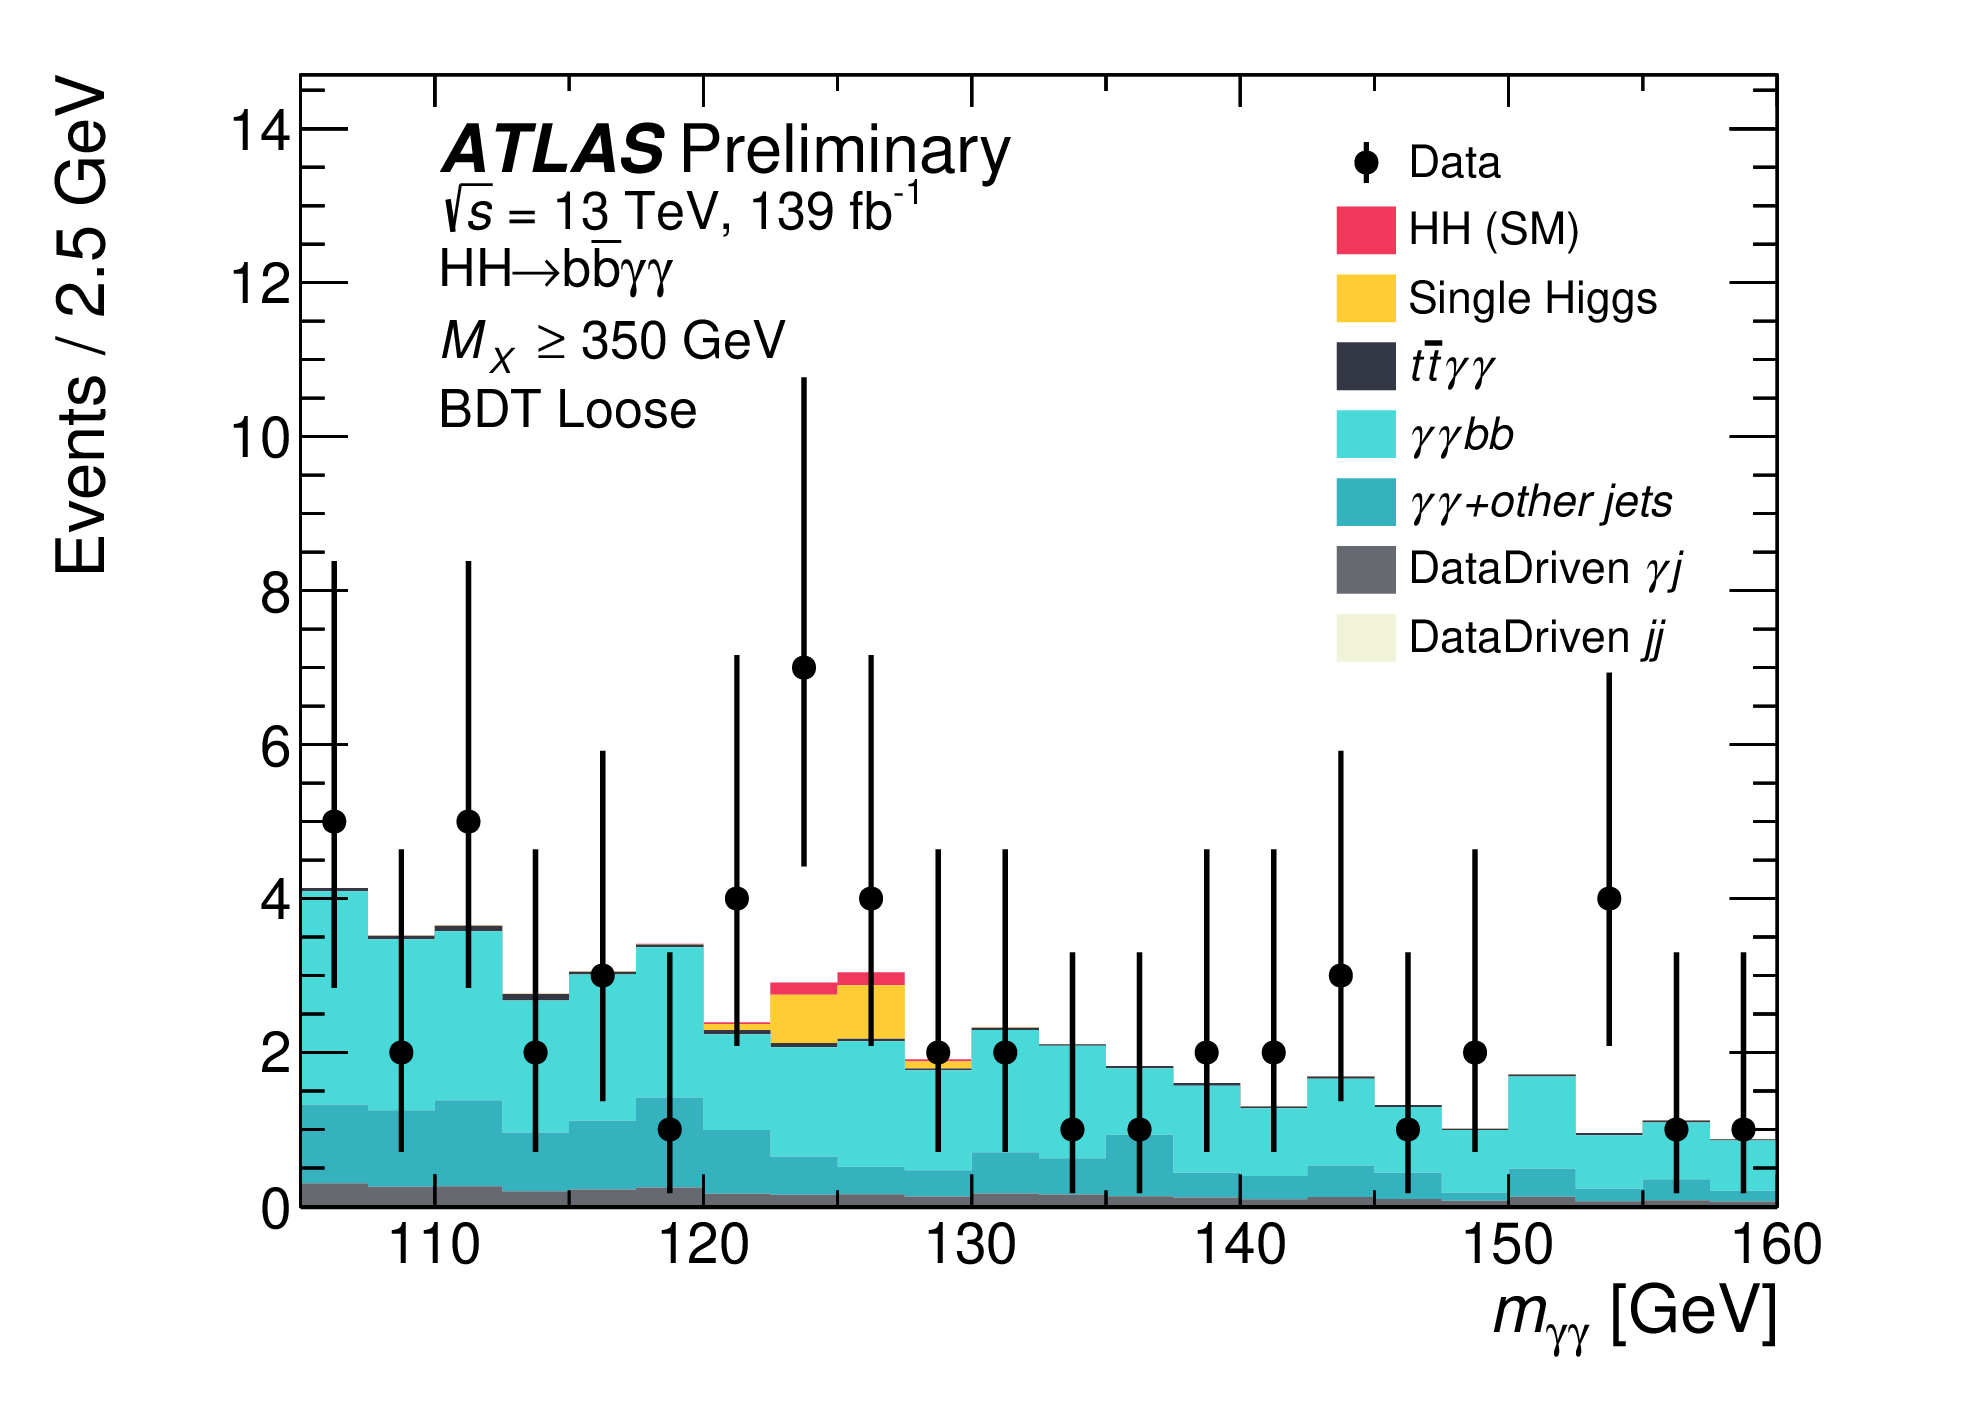
\includegraphics[width=0.35\textwidth]{BackUp/Part3/Img/High_mass_BDT_loose_data.png}}\\
    \subfloat{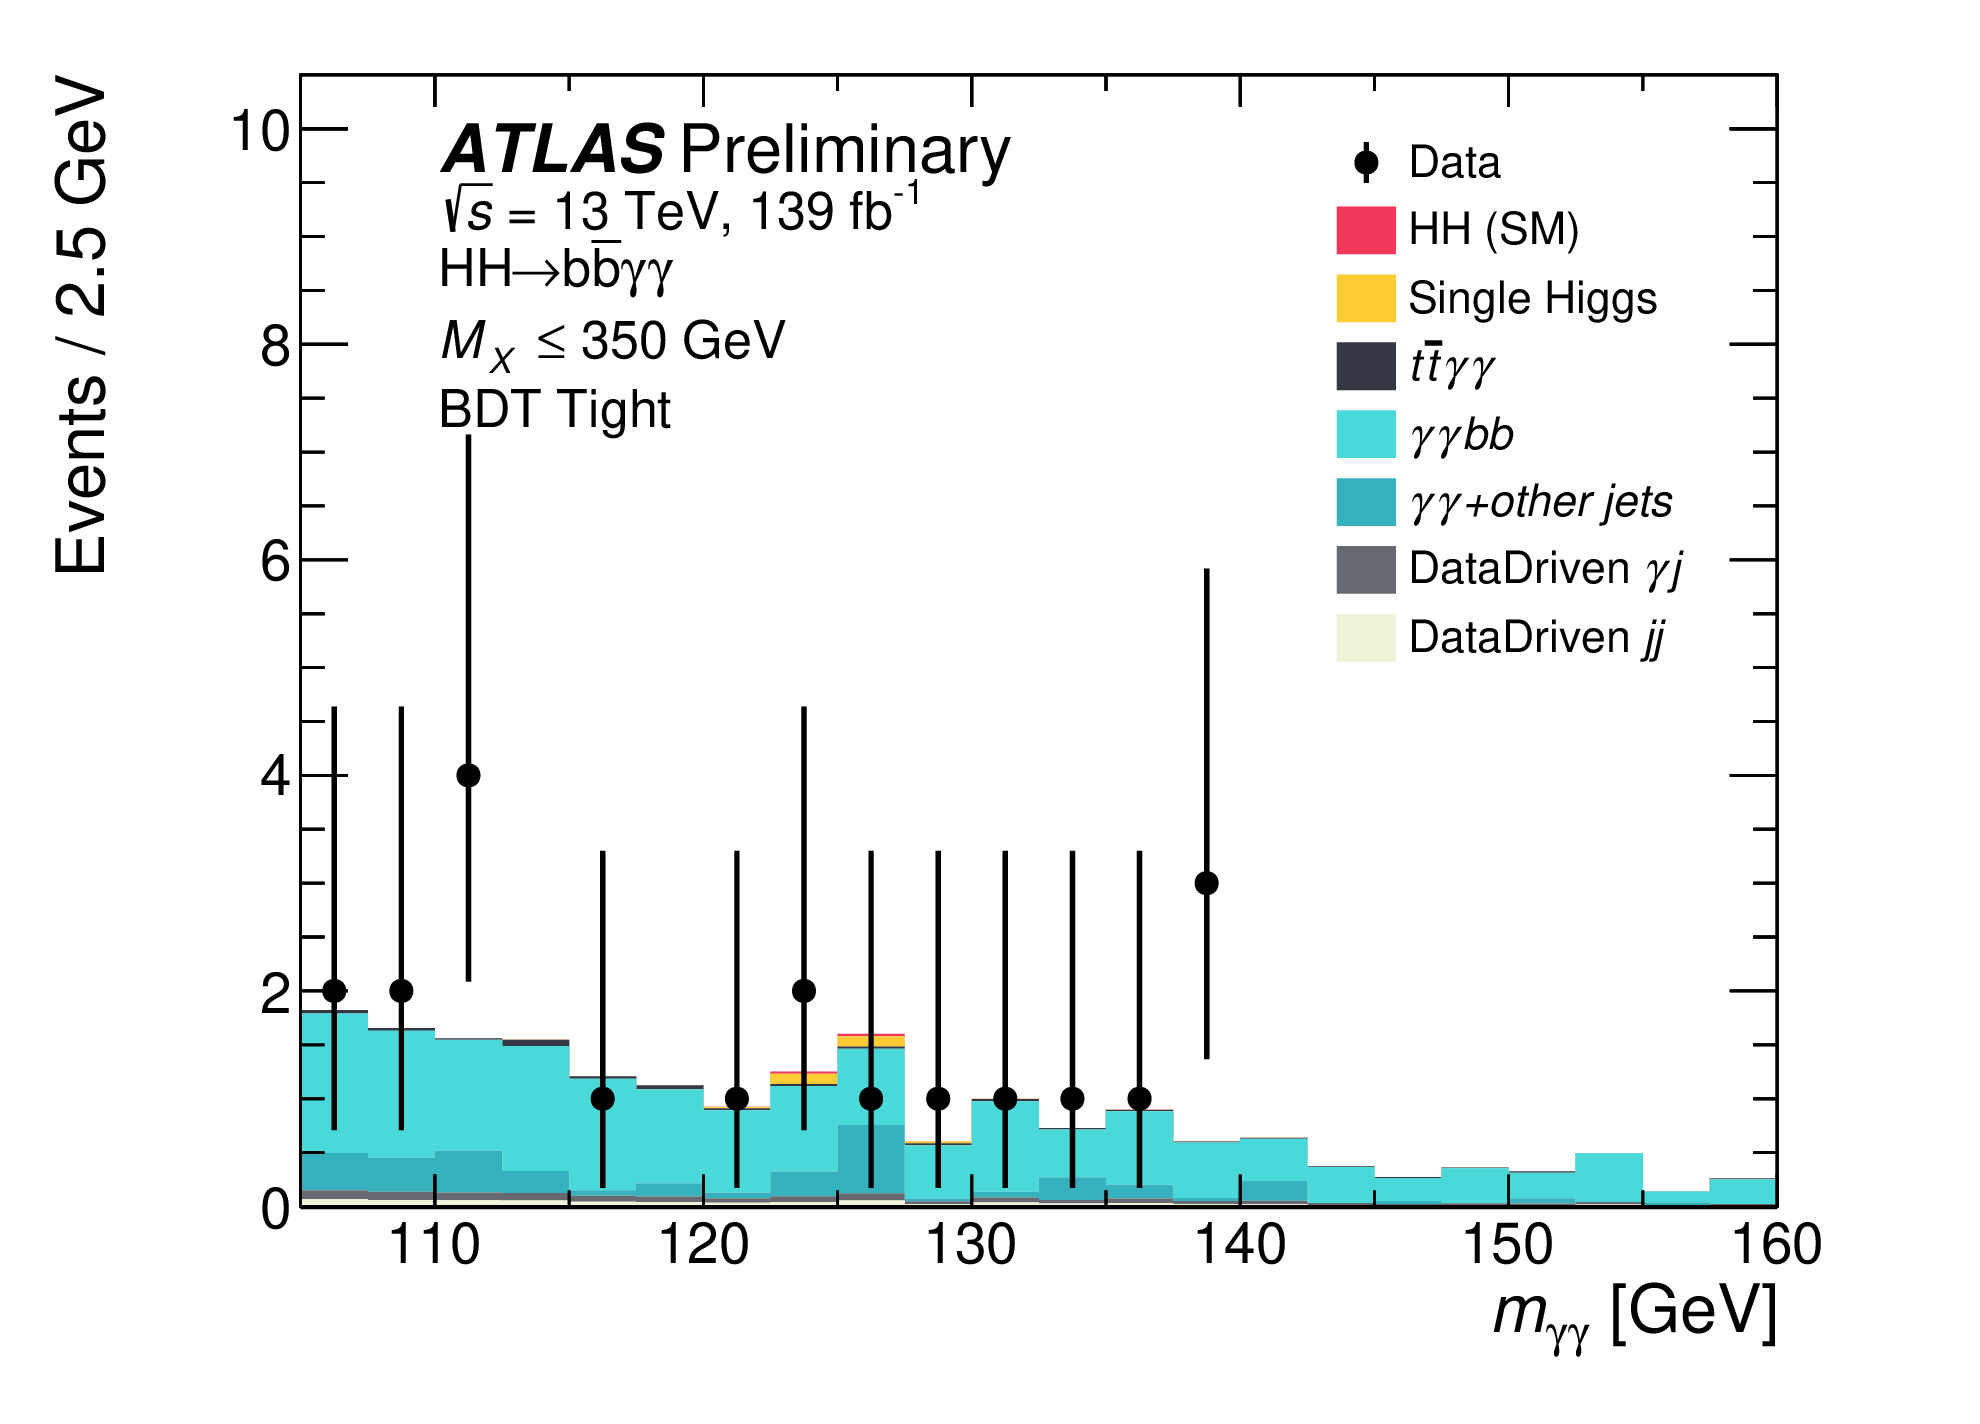
\includegraphics[width=0.35\textwidth]{BackUp/Part3/Img/Low_mass_BDT_tight_data.png}}
    \subfloat{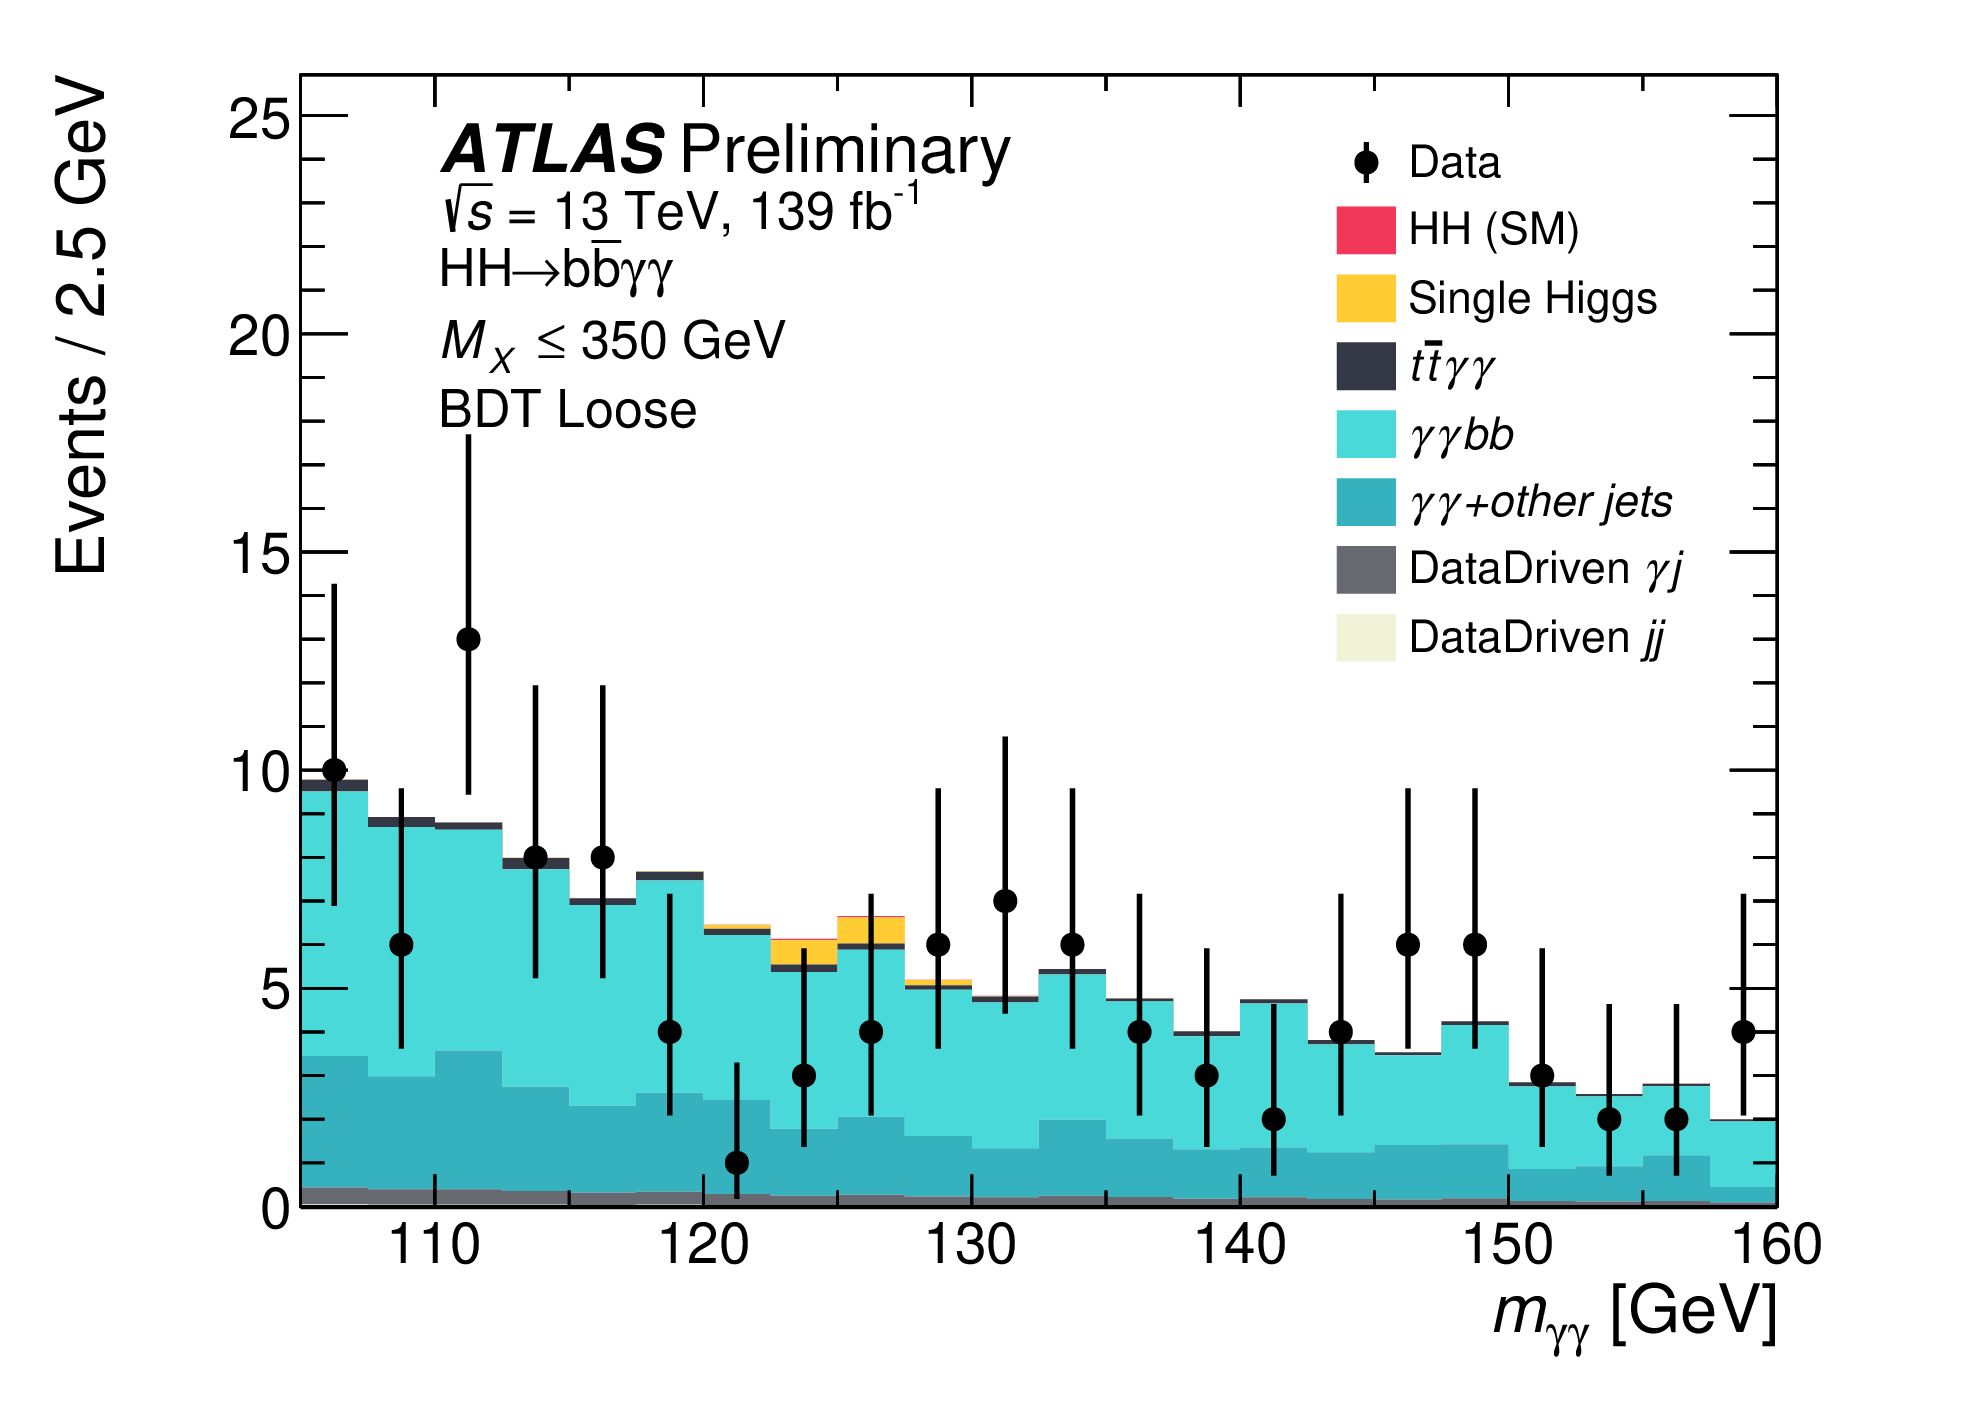
\includegraphics[width=0.35\textwidth]{BackUp/Part3/Img/Low_mass_BDT_loose_data.png}}
\end{figure}
\end{frame}

\begin{frame}{Statistical model}

\begin{equation*}
    \mathcal{L}=\prod_{c}\left(Pois\left(n_{c}
    \mid N_{c}(\theta)\right) \cdot \prod_{i=1}^{n_{c}}
    f_{c}\left(m_{\gamma \gamma}^{i}, \theta\right) \cdot G(\theta)\right),
\end{equation*}
\begin{equation*}
    N_{c}(\theta)=\mu \cdot N_{\mathrm{HH},
    \mathrm{c}}\left(\theta_{yield }\right)+N_{\mathrm{H},
    \mathrm{c}}\left(\theta_{yield }\right)+N_{\mathrm{SS},
    \mathrm{c}} \cdot \theta_{\mathrm{SS},
    \mathrm{c}}+N_{\text{continuum} , \mathrm{c}},
\end{equation*}
\begin{equation*}
    \tilde{q}_{\mu}=\left\{\begin{array}{ll}
-2 \log \frac{L(\mu, \hat{\hat{\theta}}({\mu}))}{L(0, \hat{\hat{\theta}}(0))} & \hat{\mu}<0 \\
-2 \log \frac{L(\mu, \hat{\hat{\theta}}({\mu}))}{L(\hat{\mu}, \hat{\theta})} & 0 \leq \hat{\mu} \leq \mu \\
0 & \hat{\mu}>\mu
\end{array}\right.
\end{equation*}
\end{frame}

\begin{frame}{Modelling and Spurious Signal}
\begin{columns}
\column{0.5\textwidth}
\begin{itemize}
    \item Biases related to the choice quantified through the Spurious Signal (SS) method:
    \begin{itemize}
        \item Measure residual fitted $N_{SS}$ in continuum MC: $n_{sig} \times PDF_{sig} + n_{bkg} \times PDF_{bkg}$
        \item $N_{SS} = \max|n_{sig}(m_{H})|$ : $m_{H}$ vary from 121 to 129 with step of 1 GeV
        \item Relaxed SS criteria (allowing $2\sigma$ local statistical fluctuation) is used because of lack of statistics. 
        \begin{equation*}
        \zeta_{\mathrm{SS}}=\left\{\begin{array}{ll}
        N_{\mathrm{SS}}+2 \Delta_{\mathrm{MC}}, & N_{\mathrm{SS}}+2 \Delta_{\mathrm{MC}}<0 \\
        N_{\mathrm{SS}}-2 \Delta_{\mathrm{MC}}, & N_{\mathrm{SS}}-2 \Delta_{\mathrm{MC}}>0 \\
        0, & \  otherwise 
        \end{array}\right.
        \end{equation*}
    \end{itemize}
    \item Functional form chosen: \textbf{Exponential} 
    \item The fitted $N_{SS}$ are used as systematic uncertainties on the signal yield
\end{itemize}

\column{0.5\textwidth}

\begin{table}[]
    \centering
    \begin{tabular}{lc}
    \hline\hline
       Category  & $N_{SS}$ \\
       \hline
       High mass BDT tight &  0.688 \\
       High mass BDT loose &  0.990 \\
       Low mass BDT tight  &  0.594 \\
       Low mass BDT loose  & 1.088 \\
       \hline\hline
    \end{tabular}
\end{table}

\end{columns}
\end{frame}

\begin{frame}{$b$-jet energy calibration systematic}
    \begin{itemize}
        \item $\mu$-in-jet systematic negligible from Run-1 in ZH
        \item Impact of $b$-tagging WP on $p_T$Reco, as systematic
        \begin{itemize}
            \item three variations of the $p_T$Reco correction, using 60\%, 70\% and 85\% $b$-tagging WP.
            \item relative impact on the yield $\to$ systematic uncertainty
            \item largest systematic, same order as the flavour tagging uncertainty
        \end{itemize}
    \end{itemize}
    \begin{table}[]
        \centering
        \begin{tabular}{lc}
        \hline\hline
            $p_T$-Reco variation & \% relative effect to nominal \\
        \hline    
            60\% WP & $\pm$ 0.094 \\
            70\% WP & $\pm$ 0.065 \\
            85\% WP & $\pm$ 0.12 \\
        \hline\hline
        \end{tabular}
    \end{table}
    
\end{frame}
\begin{frame}{$p_T$Reco as function of $b$-tagging WPs}
    \begin{figure}
        \centering
        \subfloat{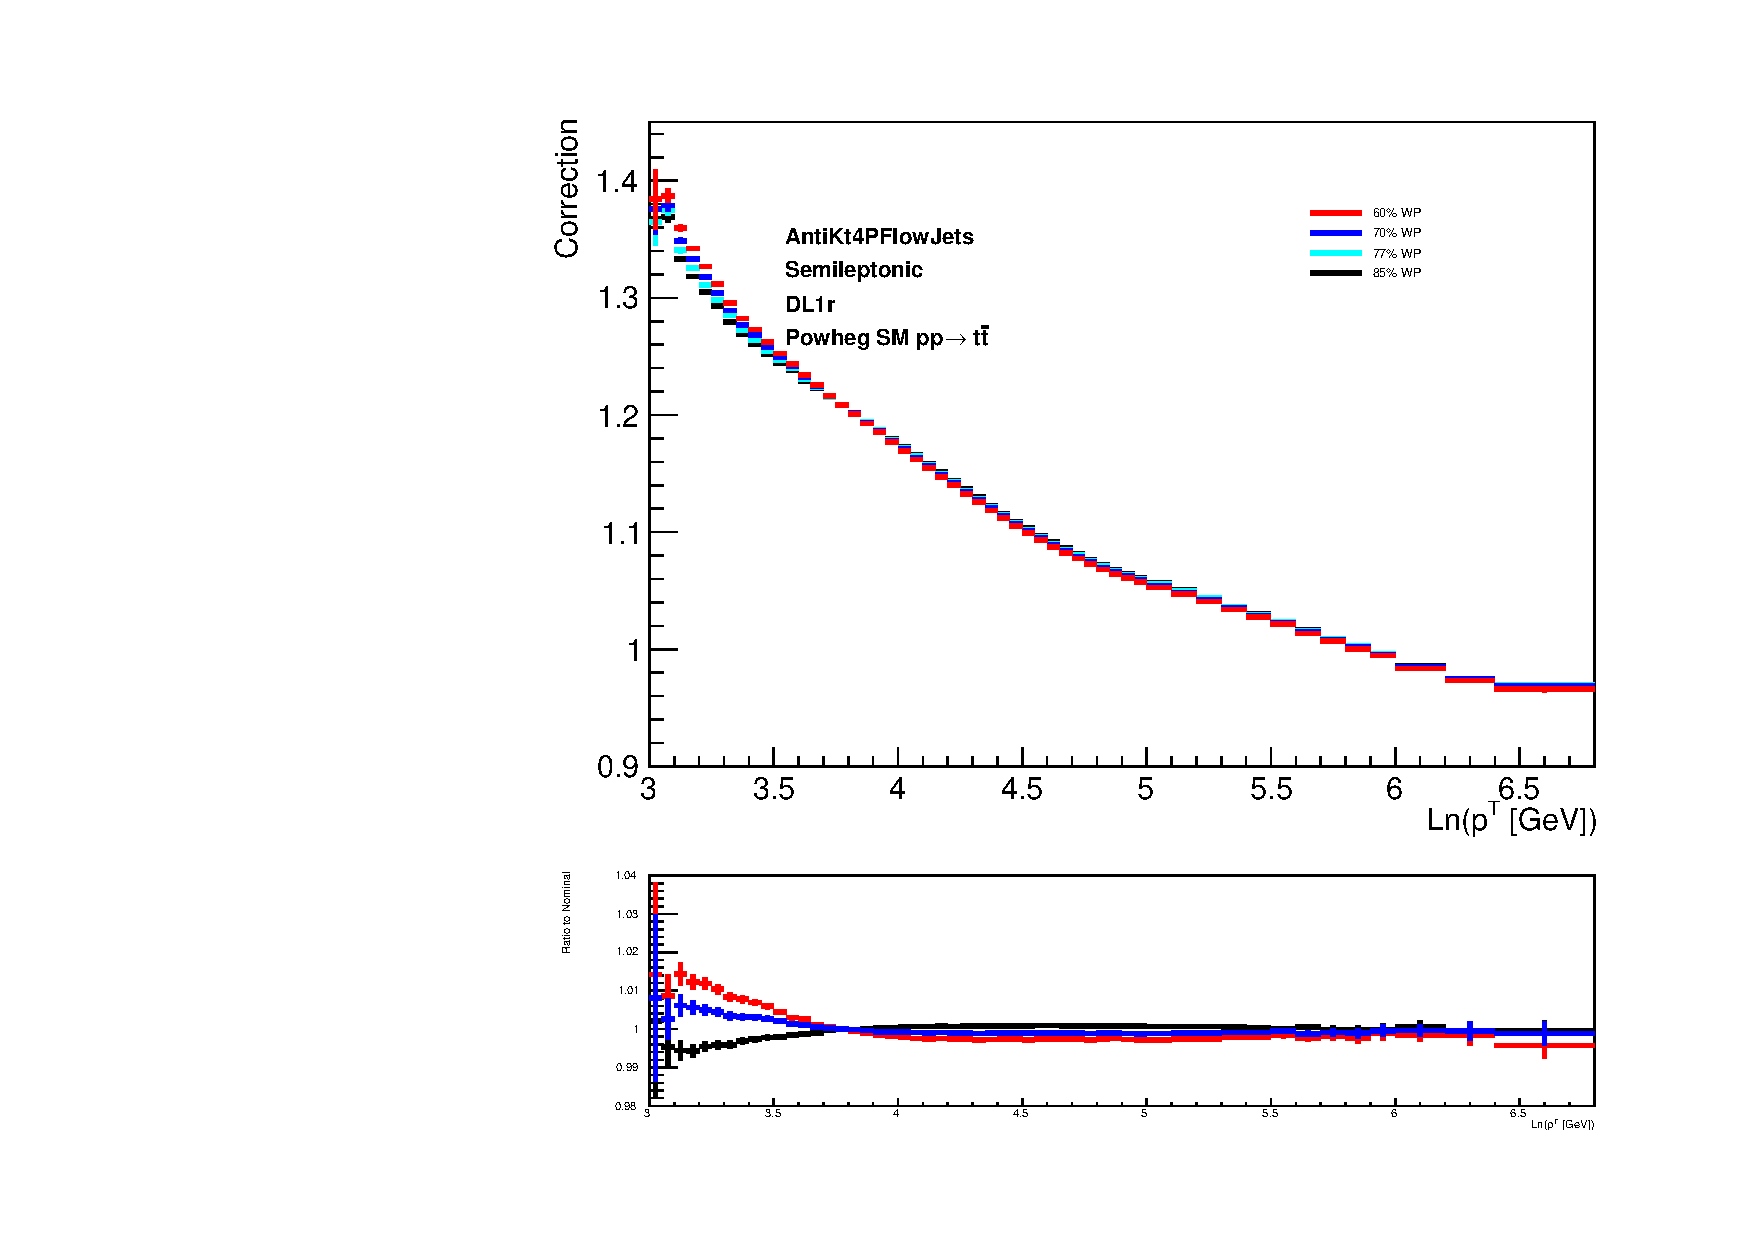
\includegraphics[width=0.55\textwidth]{BackUp/Part3/Img/Semileptonic.pdf}}
        \subfloat{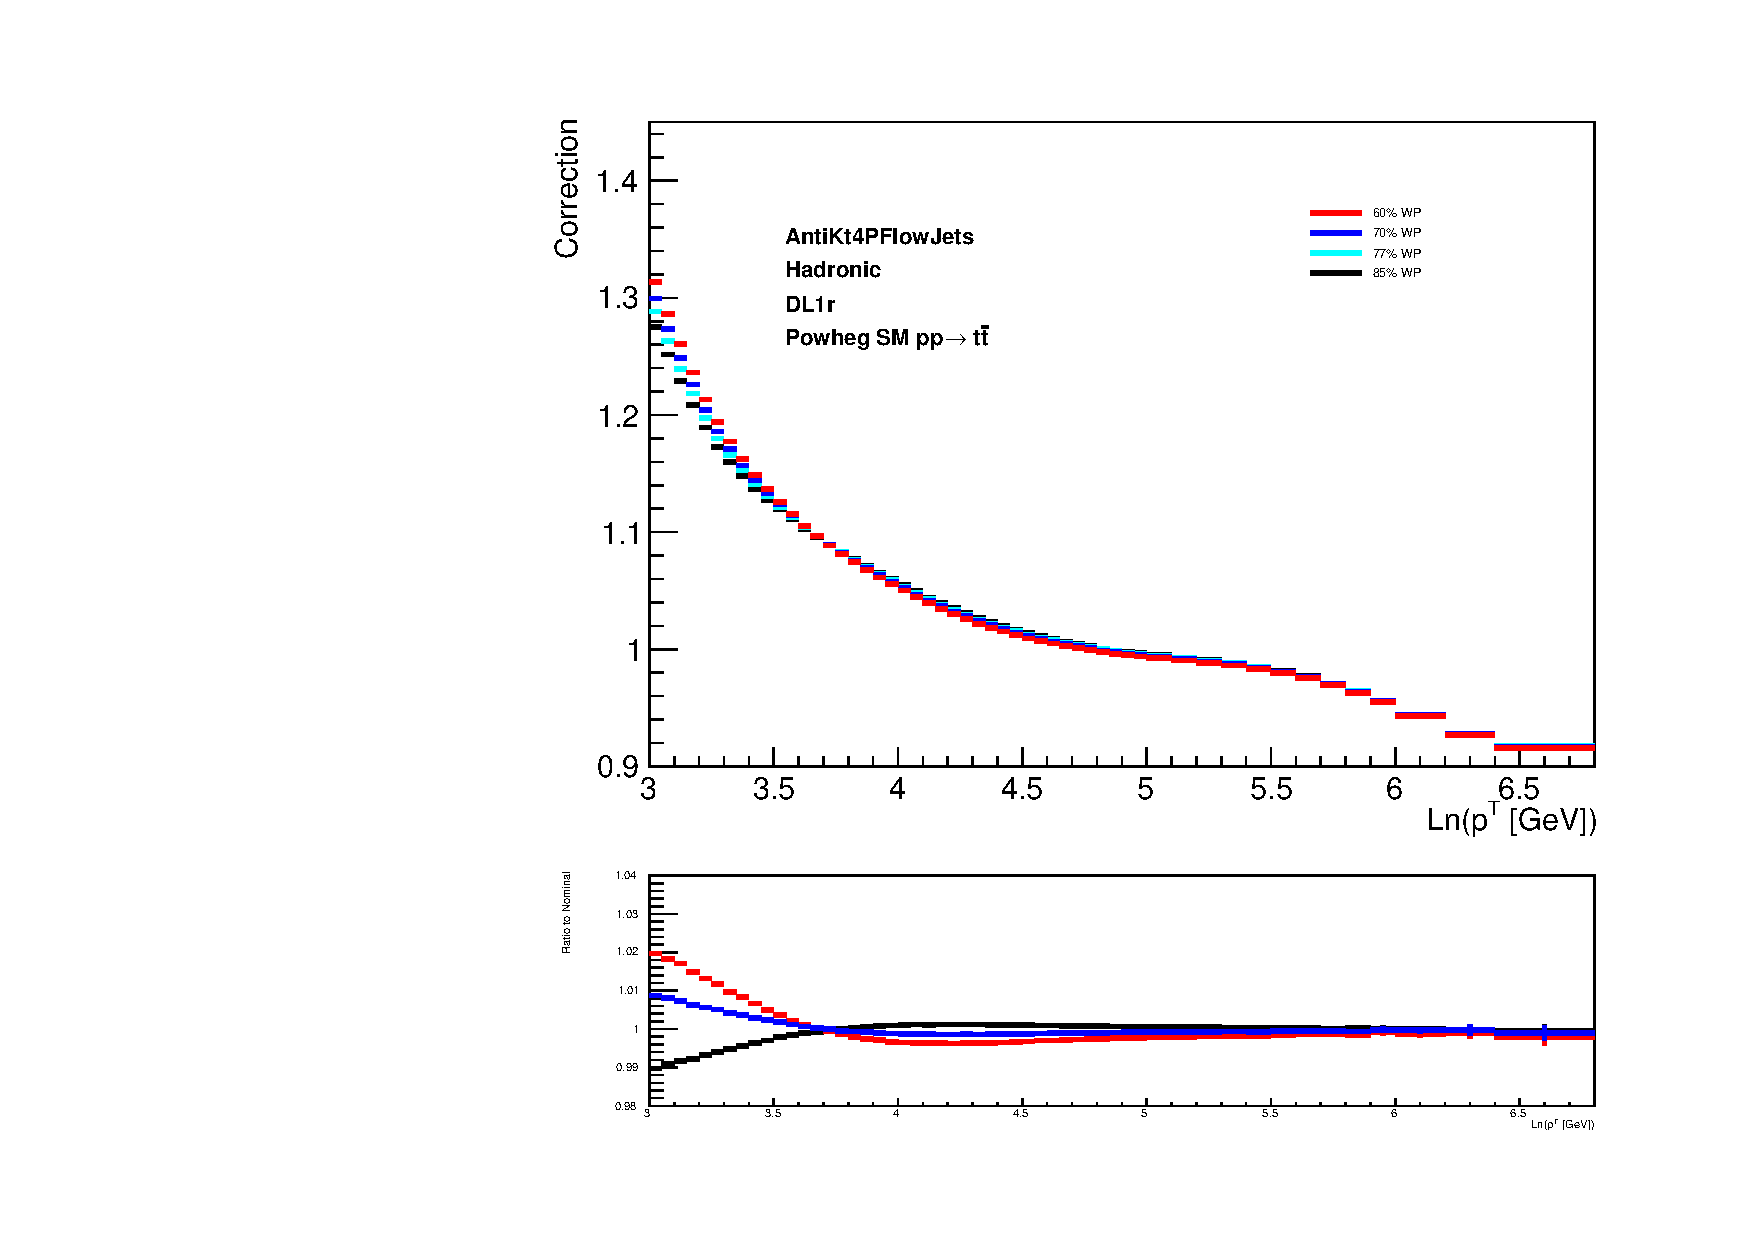
\includegraphics[width=0.55\textwidth]{BackUp/Part3/Img/Hadronic.pdf}}
    \end{figure}
\end{frame}

\begin{frame}{background-only fit}
\begin{figure}
    \centering
    \subfloat{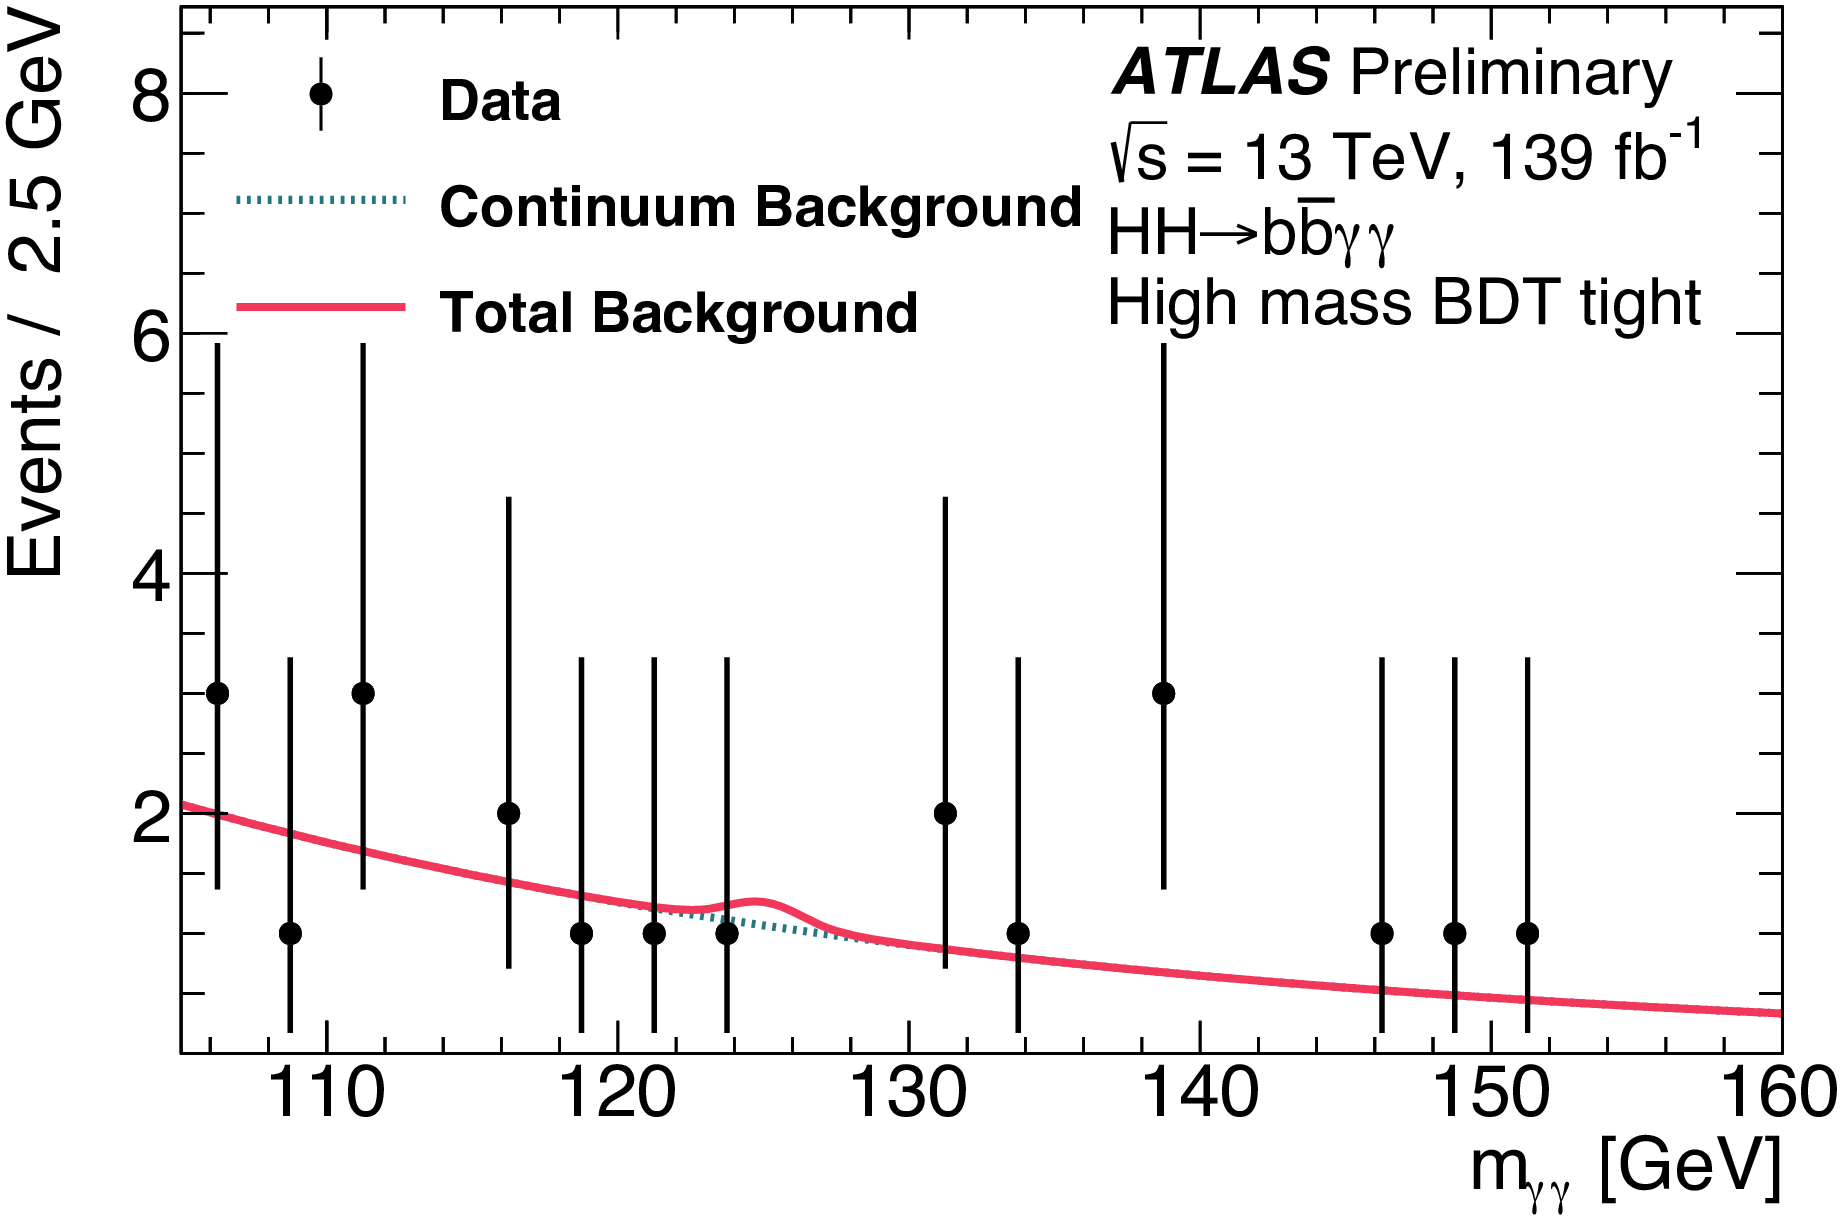
\includegraphics[width=0.35\textwidth]{BackUp/Part3/Img/High_mass_BDT_tight.png}}
    \subfloat{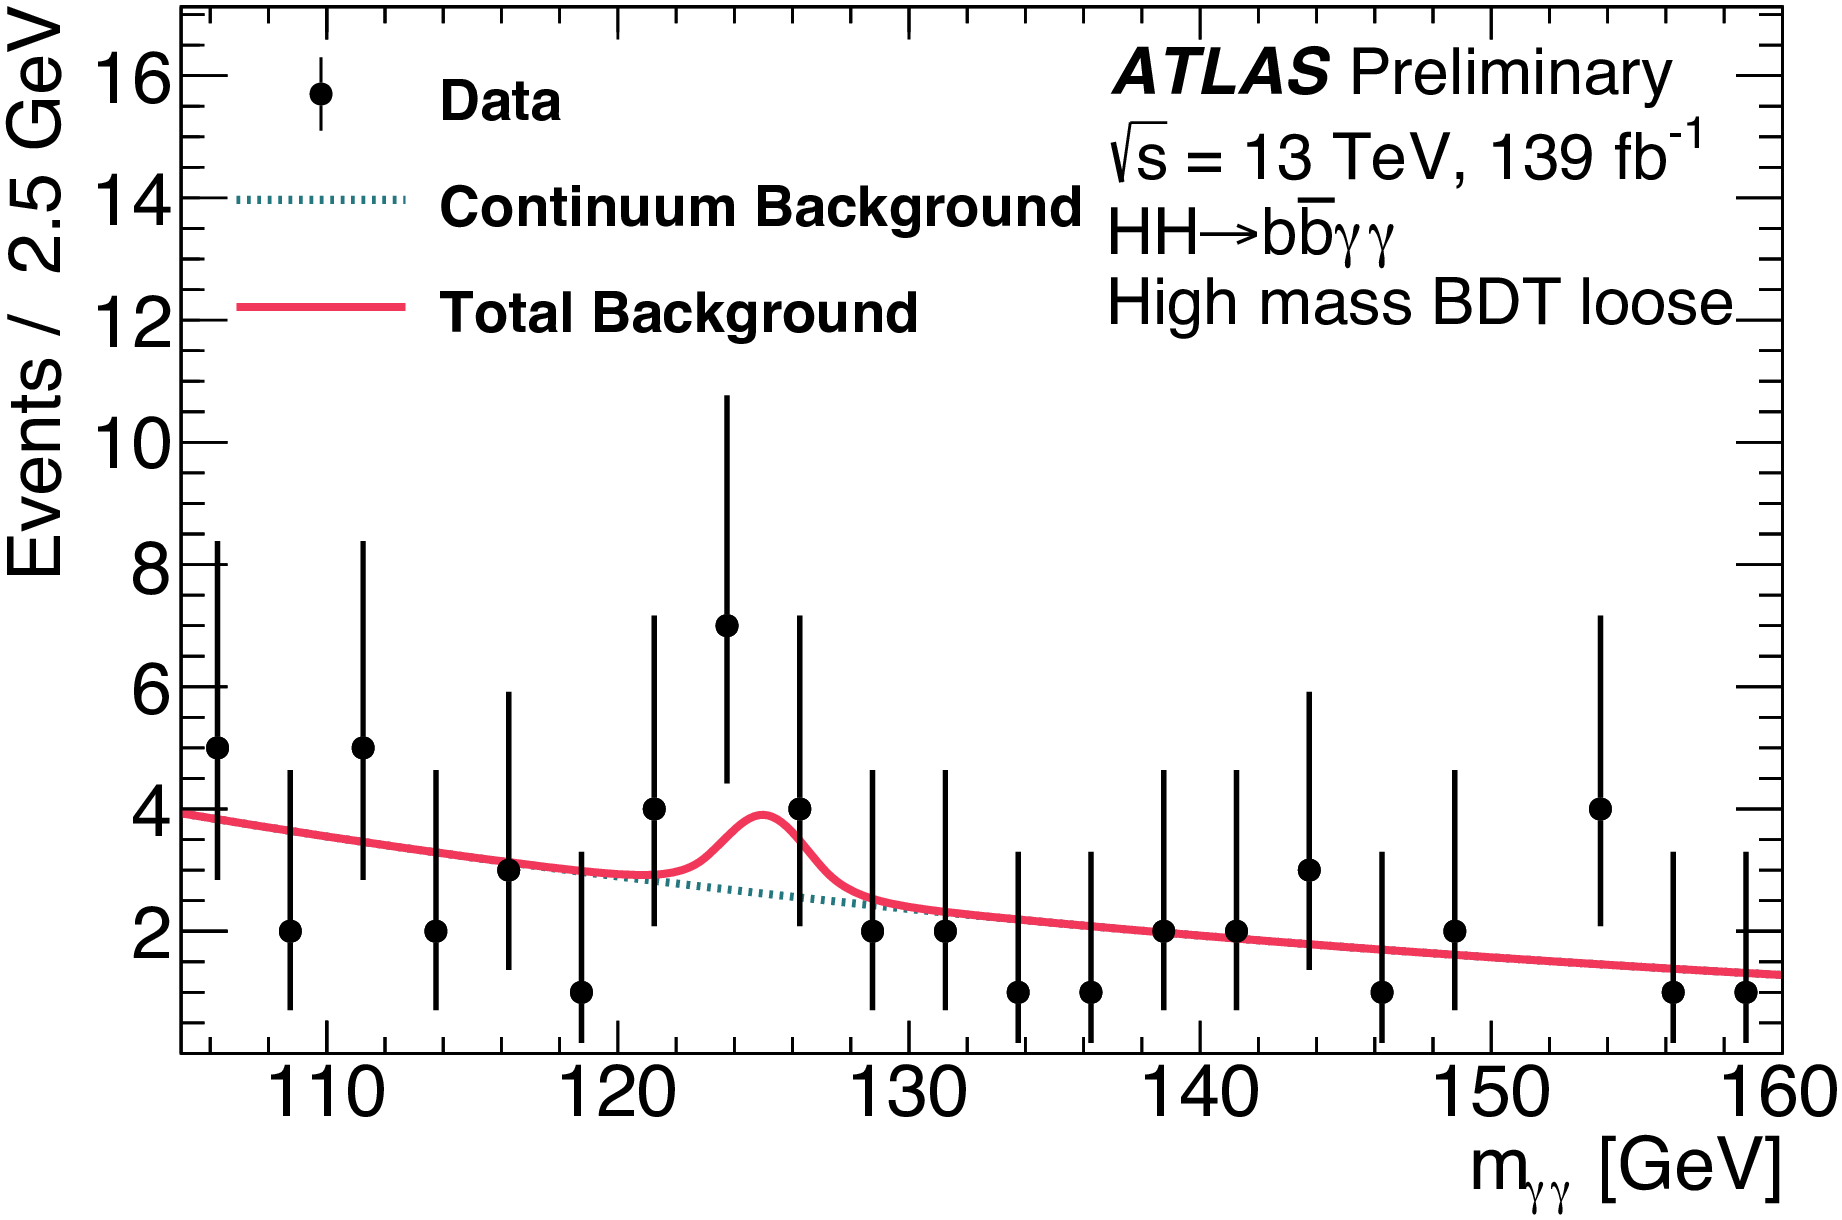
\includegraphics[width=0.35\textwidth]{BackUp/Part3/Img/High_mass_BDT_loose.png}}\\
    \subfloat{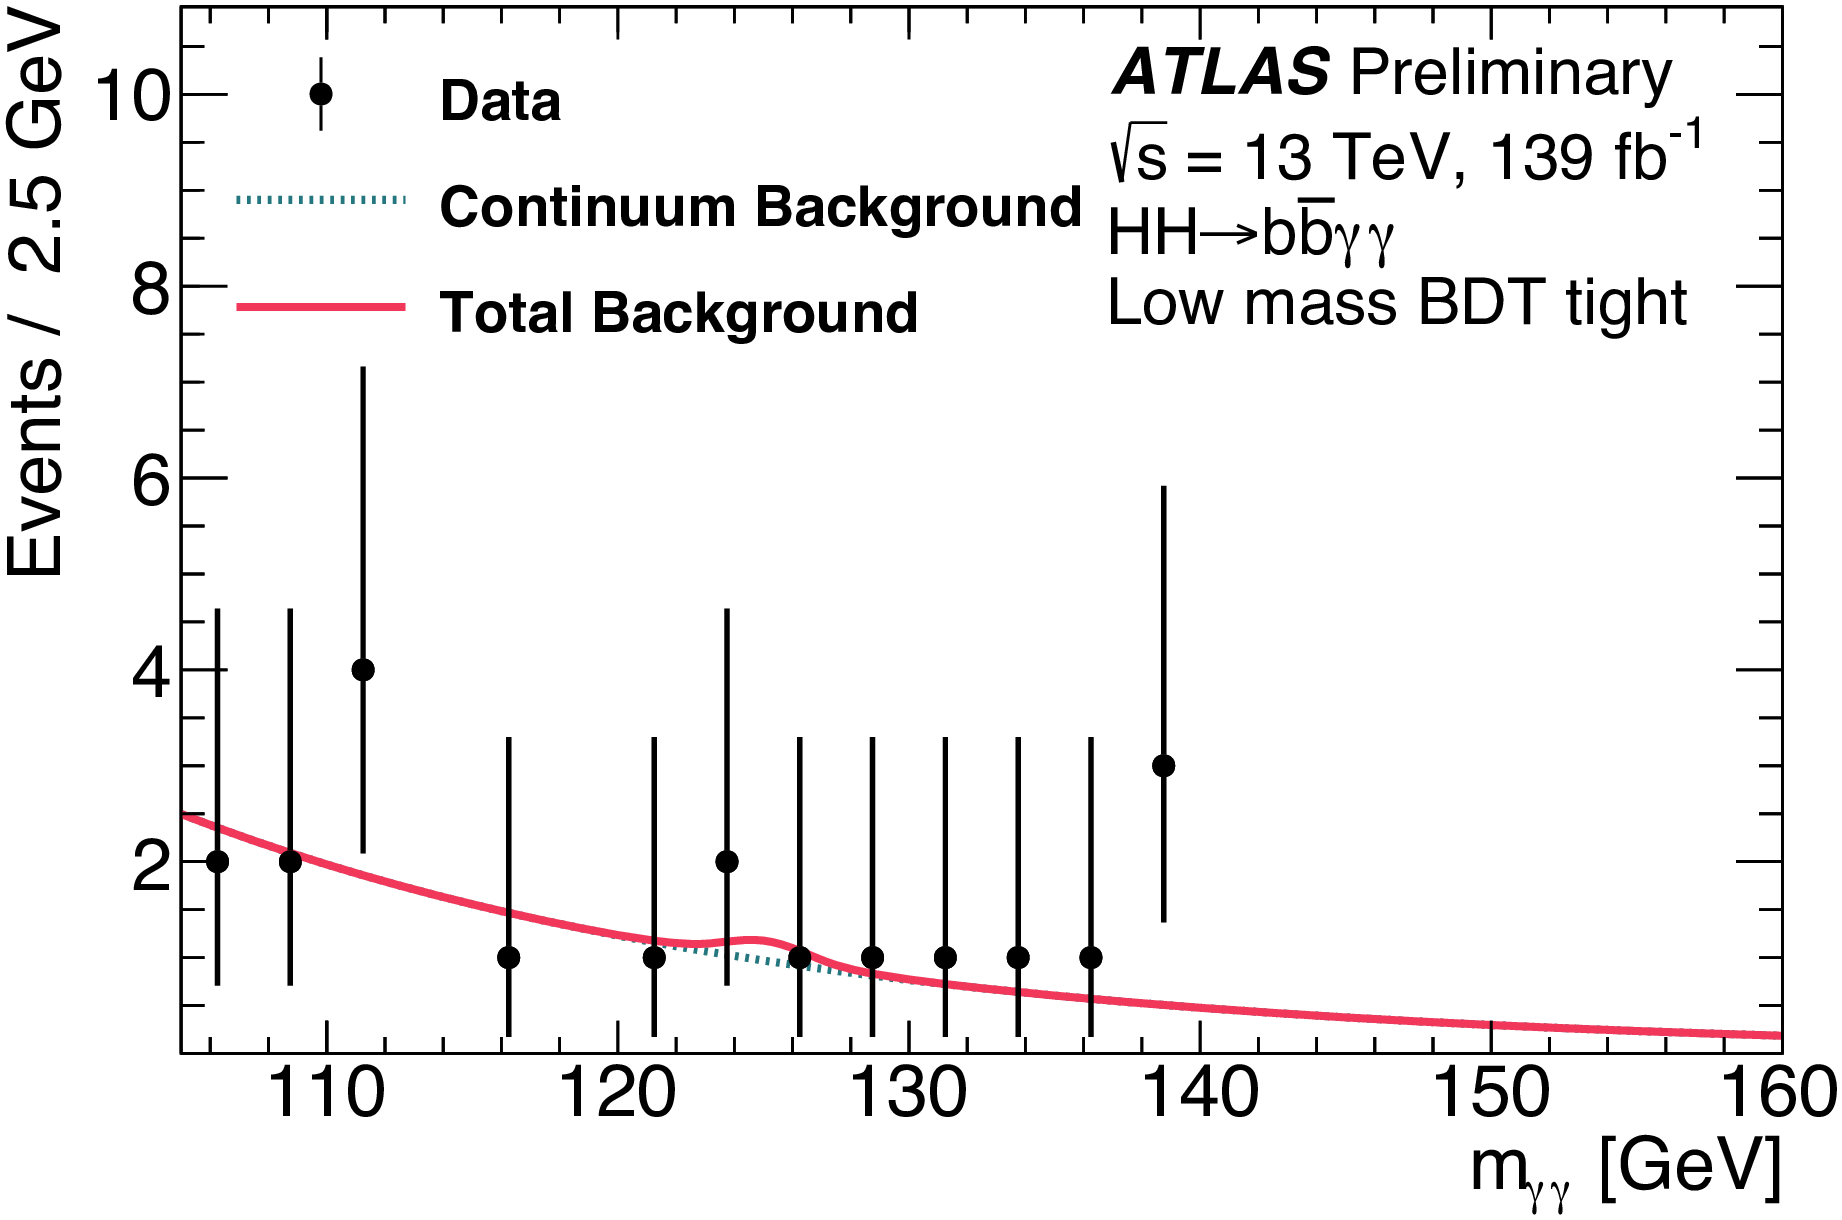
\includegraphics[width=0.35\textwidth]{BackUp/Part3/Img/Low_mass_BDT_tight.png}}
    \subfloat{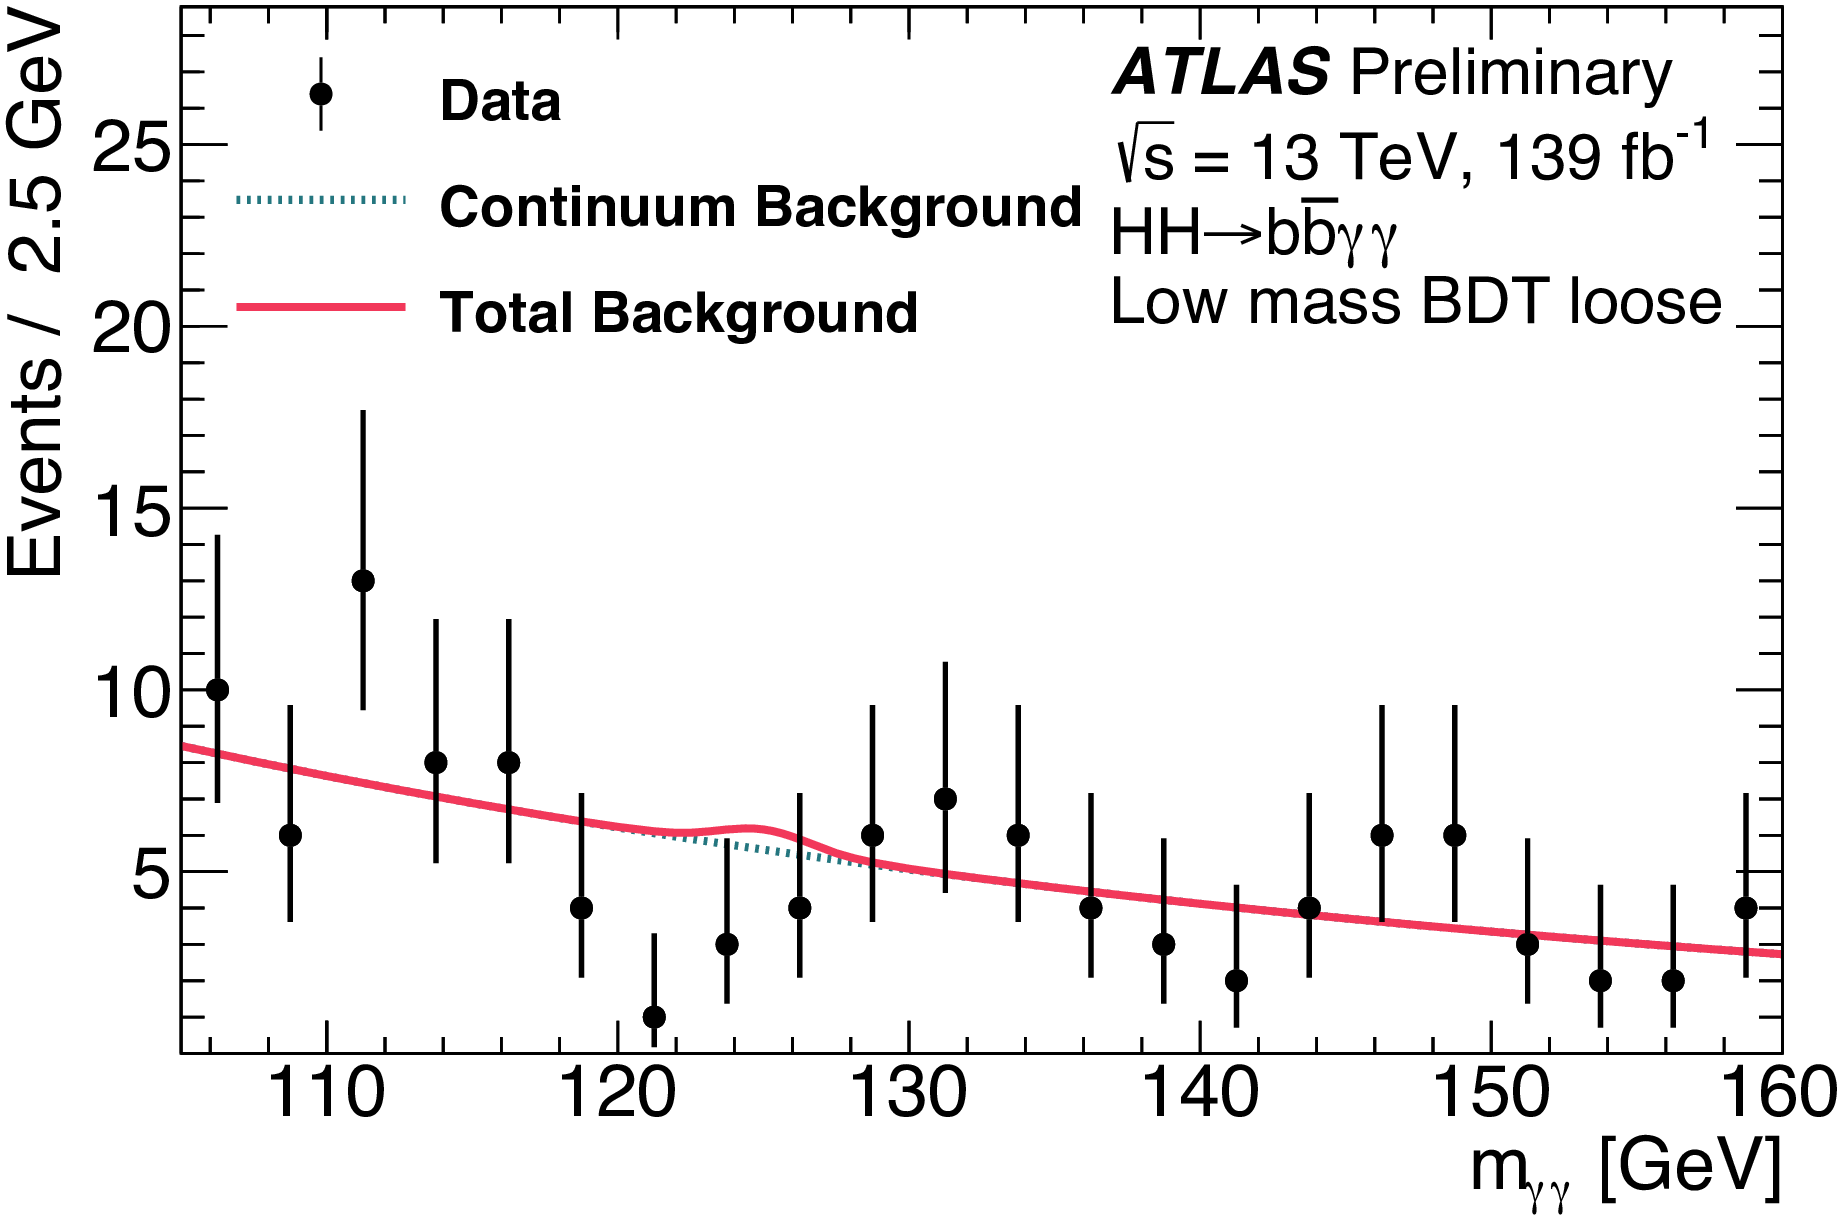
\includegraphics[width=0.35\textwidth]{BackUp/Part3/Img/Low_mass_BDT_loose.png}}
\end{figure}    
\end{frame}

\begin{frame}{Observed events}

\begin{figure}
    \centering
    \includegraphics[width=0.8\textwidth]{BackUp/Part3/Img/Events.png}
\end{figure}    
\end{frame}

\begin{frame}{Systematic impact}
\begin{figure}
    \centering
    \includegraphics[width=0.8\textwidth]{BackUp/Part3/Img/Systematics.png}
\end{figure}    
\end{frame}

\begin{frame}{Expected limit: Stat. Only vs Stat.+Syst.}
\begin{columns}
\column{0.5\textwidth}
\begin{figure}
    \centering
    \includegraphics[width=1.\textwidth]{BackUp/Part3/Img/kappa_lambda_stat_vs_sys.pdf}
\end{figure}
\column{0.5\textwidth}

\begin{table}[htbp]
    \centering
    \begin{tabular}{lcc}
    \hline \hline 
         & Stat. Only & Stat.+Syst. \\
         \hline
        $\sigma_{HH}/\sigma_{HH}^{SM}$ limit & 5.3 & 5.5  \\
         $\kappa_{\lambda}$ interval &  [-2.3, 7.6] &  [-2.4, 7.7]   \\
         \hline \hline
    \end{tabular}
\end{table}
\begin{table}[htbp]
    \centering
    \begin{tabular}{lc}
        \hline\hline
        Category &  $\sigma_{HH}/\sigma_{HH}^{SM}$ limit \\
        \hline
        High mass, High BDT &  5.8 \\
        High mass, Low BDT &  21.0  \\
        Low mass, High BDT &  102.9 \\
        Low mass, Low BDT  &  125.6 \\
        \hline 
        Combined & 5.5 \\
        \hline\hline
    \end{tabular}
\end{table}

\end{columns}  
\end{frame}

\begin{frame}{$\kappa_{\lambda}$ likelihood scan}

\begin{columns}
\column{0.5\textwidth}
\begin{figure}
    \centering
    \includegraphics[width=1.\textwidth]{BackUp/Part3/Img/figures_Results_scan_hhyybb_kl.pdf}
\end{figure}    
\column{0.5\textwidth}
\begin{itemize}
    \item best-fit $\kappa_{\lambda}$ is 2.7$^{+2.1}_{-2.2}$
    \item $\mu_{HH} = 1 \pm 2.37$ for SM
\end{itemize}
\begin{table}[]
    \centering
    \begin{tabular}{lcc}
    \hline\hline
        & 1$\sigma$ CI & 2$\sigma$ CI  \\
    \hline    
        Expected & [-1.4, 6.4] & [-3.1, 8.2] \\
        Observed & [0.5, 4.7] & [-1.4, 6.5]\\
    \hline\hline    
    \end{tabular}

\end{table}
\end{columns}    
\end{frame}

\begin{frame}{Combination with CMS}
\begin{columns}
\column{0.5\textwidth}
\begin{itemize}
    \item ATLAS+CMS $\sim \times$2 139 fb$^{-1}$
    \item Expected 95\% CL limit on $\sigma_{HH}$ of 3.4
\end{itemize}
\column{0.5\textwidth}
\begin{figure}
    \centering
    \includegraphics[width=1.\textwidth]{BackUp/Part3/Img/kappa_lambda_ATLAS_CMS_stat.pdf}
\end{figure}
\end{columns}
\end{frame}

\begin{frame}{full Run-2 HH$\to b\bar{b} \tau^+\tau^-$}
\begin{columns}
\column{0.5\textwidth}
\href{https://atlas.web.cern.ch/Atlas/GROUPS/PHYSICS/CONFNOTES/ATLAS-CONF-2021-030/}{ATLAS-CONF-2021-030}
\begin{itemize}
    \item Relies on:
    \begin{itemize}
        \item $\tau_{had}\tau_{had}$: Single and Double tau trigger
        \item $\tau_{lep}\tau_{had}$: Single lepton an lepton+tau trigger
    \end{itemize}
    \item backgrounds:
    \begin{itemize}
        \item \textbf{true $\tau$}: $t\bar{t}$ and Z+HF, from Monte Carlo and normalization from data
        \item \textbf{fake $\tau$}: $t\bar{t}$ and multi-jet, data driven
    \end{itemize}
    \item 3 MVA categories: 
    \begin{itemize}
        \item $\tau_{had}\tau_{had}$
        \item $\tau_{lep}\tau_{had}$
        \item Z+HF background control
    \end{itemize}
    \item fit of MVA outputs
\end{itemize}


\column{0.5\textwidth}
\begin{figure}
    \centering
    \includegraphics[width=1.\textwidth]{BackUp/Part3/Img/tautau_results.png}
\end{figure}

\begin{itemize}
    \item $\times$4 improvement w.r.t early Run-2 (12.7$\times$SM)
    \item large systematic from background modelling
\end{itemize}
\end{columns}
\end{frame}

\begin{frame}{full Run-2 HH$\to b\bar{b} \tau^+\tau^-$}
    
\begin{figure}
    \centering
    \subfloat{\includegraphics[width=0.3\textwidth]{BackUp/Part3/Img/BDT_tautau_hadhad.png}}
    \subfloat{\includegraphics[width=0.3\textwidth]{BackUp/Part3/Img/BDT_tautau_lephad_SLT.png}} 
    \subfloat{\includegraphics[width=0.3\textwidth]{BackUp/Part3/Img/BDT_tautau_leptau_DLT.png}}
\end{figure}
\end{frame}

\begin{frame}{Early Run-2 combination}
\begin{figure}
    \centering
    \includegraphics[width=0.6\textwidth]{BackUp/Part3/Img/XSec_Comb_36.png}
\end{figure}

\end{frame}

\begin{frame}{First full Run-2 combination}
    
\begin{figure}
    \centering
    \includegraphics[width=0.6\textwidth]{BackUp/Part3/Img/full_Run_2_comb.png}
\end{figure}    
\end{frame}
\begin{frame}{Single Higgs vs $\kappa_{\lambda}$}
    \begin{figure}
        \centering
        \includegraphics[width=0.6\textwidth]{BackUp/Part3/Img/Single_Higgs_as_kl.png}
    \end{figure}
\end{frame}

\begin{frame}{H+HH }
\begin{columns}
\column{0.5\textwidth}
\begin{figure}
    \centering
    \includegraphics[width=1\textwidth]{BackUp/Part3/Img/H_HH_combination.png}
\end{figure}

\column{0.5\textwidth}
\begin{figure}
    \centering
    \includegraphics[width=1\textwidth]{BackUp/Part3/Img/H_HH_combination_kt_kl.png}
\end{figure}

\end{columns}
\end{frame}